\documentclass[12pt, oneside]{article}

\usepackage[letterpaper, scale=0.89, centering]{geometry}
\usepackage{fancyhdr}
\setlength{\parindent}{0em}
\setlength{\parskip}{1em}

\pagestyle{fancy}
\fancyhf{}
\renewcommand{\headrulewidth}{0pt}
\rfoot{\href{https://creativecommons.org/licenses/by-nc-sa/2.0/}{CC BY-NC-SA 2.0} Version \today~(\thepage)}

\usepackage{amssymb,amsmath,pifont,amsfonts,comment,enumerate,enumitem}
\usepackage{currfile,xstring,hyperref,tabularx,graphicx,wasysym}
\usepackage[labelformat=empty]{caption}
\usepackage[dvipsnames,table]{xcolor}
\usepackage{multicol,multirow,array,listings,tabularx,lastpage,textcomp,booktabs}

\lstnewenvironment{algorithm}[1][] {   
    \lstset{ mathescape=true,
        frame=tB,
        numbers=left, 
        numberstyle=\tiny,
        basicstyle=\rmfamily\scriptsize, 
        keywordstyle=\color{black}\bfseries,
        keywords={,procedure, div, for, to, input, output, return, datatype, function, in, if, else, foreach, while, begin, end, }
        numbers=left,
        xleftmargin=.04\textwidth,
        #1
    }
}
{}
\lstnewenvironment{java}[1][]
{   
    \lstset{
        language=java,
        mathescape=true,
        frame=tB,
        numbers=left, 
        numberstyle=\tiny,
        basicstyle=\ttfamily\scriptsize, 
        keywordstyle=\color{black}\bfseries,
        keywords={, int, double, for, return, if, else, while, }
        numbers=left,
        xleftmargin=.04\textwidth,
        #1
    }
}
{}

\newcommand\abs[1]{\lvert~#1~\rvert}
\newcommand{\st}{\mid}

\newcommand{\A}[0]{\texttt{A}}
\newcommand{\C}[0]{\texttt{C}}
\newcommand{\G}[0]{\texttt{G}}
\newcommand{\U}[0]{\texttt{U}}

\newcommand{\cmark}{\ding{51}}
\newcommand{\xmark}{\ding{55}}

 
\begin{document}
\begin{flushright}
    \StrBefore{\currfilename}{.}
\end{flushright} 
\section*{Before we start}
If you or someone you know is suffering from food and/or housing insecurities 
there are UCSD resources here to help:

Basic Needs Office: \href{https://basicneeds.ucsd.edu/}{https://basicneeds.ucsd.edu/}

Triton Food Pantry (in the old Student Center)
is free and anonymous, and includes produce: 

\href{https://www.facebook.com/tritonfoodpantry/}{https://www.facebook.com/tritonfoodpantry/}

Mutual Aid UCSD: \href{https://mutualaiducsd.wordpress.com/}{https://mutualaiducsd.wordpress.com/}

If you find yourself in an uncomfortable situation, ask for help. 
We are committed to upholding University policies regarding nondiscrimination, sexual violence and sexual harassment.

Counseling and Psychological Services (CAPS) at 858 5343755 or \href{http://caps.ucsd.edu}{http://caps.ucsd.edu}


OPHD at (858) 534-8298, ophd@ucsd.edu , \href{http://ophd.ucsd.edu}{http://ophd.ucsd.edu}. 
CARE at Sexual Assault Resource Center at 858 5345793 sarc@ucsd.edu \href{http://care.ucsd.edu}{http://care.ucsd.edu}

\subsection*{Pandemic resilient instruction}
Fall 2021 is a transition quarter so please be patient with us as we do our best 
to serve the needs of all students while adhering to the university guidelines. 
First and foremost is the health and safety of everyone.  
Please do not come to class if you are sick or even think you might be sick.
Please reach out (minnes@eng.ucsd.edu) if you need support with extenuating circumstances.

Masks are required in class. All students who attend class must also be fully vaccinated against COVID-19
unless they have a university-approved exemption.
Campus policy requires masks and daily ``symptom screeners" for everyone and we expect all students 
to follow these rules. 


\newpage
Welcome to CSE 20: Discrete Math for Computer Science in Fall 2021! 

\section*{Themes and applications for CSE 20}
\begin{itemize}
\item {\bf Technical skepticism}: Know, select and apply appropriate computing knowledge and problem-solving techniques. 
Reason about computation and systems. 
Use mathematical techniques to solve problems. 
Determine appropriate conceptual tools to apply to new situations. 
Know when tools do not apply and try different approaches. 
Critically analyze and evaluate candidate solutions.
\item {\bf Multiple representations}: Understand, guide, shape impact of computing on society/the world. 
Connect the role of Theory CS classes to other applications (in undergraduate CS curriculum and beyond). 
Model problems using appropriate mathematical concepts.
Clearly and unambiguously communicate computational ideas using appropriate formalism. 
Translate across levels of abstraction.
\end{itemize}

{\bf Applications}: Numbers (how to represent them and use them in Computer Science), 
Recommendation systems and their roots in machine learning (with applications like Netflix),
``Under the hood" of computers (circuits, pixel color representation, data structures),
Codes and information (secret message sharing and error correction),
Bioinformatics algorithms and genomics (DNA and RNA).

\section*{Introductions}
Class website: \href{http://cseweb.ucsd.edu/classes/fa21/cse20-a}{http://cseweb.ucsd.edu/classes/fa21/cse20-a}

{\bf Pro-tip}: the URL structure is your map to finding your course website for other CSE classes.

{\bf Pro-tip}: you can use MATH109 to replace CSE20 for prerequisites and other requirements.

Instructor: Prof. Mia Minnes {\tiny{"Minnes" rhymes with Guinness}}, minnes@eng.ucsd.edu, 
\href{http://cseweb.ucsd.edu/~minnes}{http://cseweb.ucsd.edu/~minnes}

Our team: Four TAs and 10 tutors + all of you

Fill in contact info for students around you, if you'd like:
\vspace{50pt}


On a typical week: {\bf MWF} Lectures + review quizzes, {\bf T} HW due, {\bf W} Discussion, office hours, Piazza. 
Project parts will be due some weeks.

All dates are on \href{https://canvas.ucsd.edu/}{Canvas (click for link)} and details are on
 \href{https://discrete-math-for-cs.github.io/website/overview_calendar.html}{course calendar (click for link)}.

Education research: CSE 20 is participating in a project on retention and sense of community 
in UCSD majors; see \href{https://discrete-math-for-cs.github.io/files/CSInclusiveMentoringConsentFormNonCSEDataAnalysis.pdf}{research plan}. If you consent to participate in this study, no action is needed. 
If you DO NOT consent to participate in this study, or you choose to opt-out at any time during the a
cademic year, sign and submit this form to the research contact at retentionstudy@cs.ucsd.edu.


\newpage
\section*{Friday September 24}


What data should we encode about each Netflix account holder to help us make effective recommendations?

\vfill
\vfill

In machine learning, clustering can be used to group similar data for prediction and recommendation.  For example,
each Netflix user's viewing history can be represented as a $n$-tuple indicating their preferences about
movies in the database, where $n$ is the number of movies in the database.  People with similar tastes in movies can then be clustered to provide recommendations
of movies for one another.  Mathematically, clustering is based on a notion of distance between pairs of $n$-tuples.
 

In the table  below,  each row represents a user's ratings of movies: 
\cmark~(check) indicates the person liked the movie, \xmark~(x)
that they didn't, and $\bullet$ (dot) that they didn't rate it one way or 
another (neutral rating or didn't watch). Can encode
these ratings numerically with $1$ for \cmark~(check), $-1$ for \xmark~(x), 
and $0$ for $\bullet$ (dot).

\begin{center}
\begin{tabular}{c|ccc||c}
Person & Fyre & Frozen II & Picard & Ratings written as a  $3$-tuple\\
\hline
$P_1$     & \xmark & $\bullet$ & \cmark & \phantom{$(-1, 0, 1)$} \\
$P_2$     & \cmark & \cmark & \xmark & \phantom{$(1, 1, -1)$} \\
$P_3$     & \cmark & \cmark & \cmark & \phantom{$(1, 1, 1)$} \\
$P_4$     & $\bullet$ & \xmark & \cmark &  \\
\end{tabular}
\end{center} 
{\bf Conclusion}: Modeling involves choosing data types to represent and organize data

\newpage
\subsection*{Review: Week 0 Friday}
\begin{enumerate}
\item Please complete the beginning of the quarter survey \href{https://forms.gle/gvibFnNixxqcWbaU8}{https://forms.gle/gvibFnNixxqcWbaU8}
\item We want you to be familiar with class policies and procedures so you are ready to have a successful quarter. 
Please take a look at the class website http://cseweb.ucsd.edu/classes/fa21/cse20-a
and answer the questions about it on \href{http://gradescope.com}{Gradescope}.
\item Modeling: 
\begin{enumerate}
    \item {

Using the example movie database from class with the $3$ movies Fyre, Frozen II, Picard, 
which of the following is a $3$-tuple that represents the ratings of a user who liked
Frozen II? (Select all and only that apply.)

\begin{enumerate}
\item $1$
\item $(0,0,0)$
\item $[1,1,1]$
\item $\{-1, 0, 1\}$
\item $(1,-1,0)$
\item $(0,1,1)$
\item $(1,1,1,1)$
\end{enumerate} }
    \item {

Using the example movie database from class with the $3$ movies Fyre, Frozen II, Picard, 
how many distinct (different) $3$-tuples of ratings are there? 
 }
\end{enumerate}
\end{enumerate}
\newpage
\section*{Monday September 27}
\subsection*{Notation and prerequisites}


\begin{center}
\begin{tabular}{|llp{9.8cm}|}
\hline
{\bf Term} & {\bf Notation Example(s)} & {\bf We say in English \ldots } \\
\hline
sequence & $x_1, \ldots, x_n$ & A sequence $x_1$ to $x_n$ \\
summation & $\sum_{i=1}^n x_i$ or $\displaystyle{\sum_{i=1}^n x_i}$ & The sum of the terms of the sequence $x_1$ to $x_n$ \\
&&\\
all reals & $\mathbb{R}$ & The (set of all) real numbers (numbers on the number line)\\
all integers & $\mathbb{Z}$ & The (set of all) integers (whole numbers including negatives, zero, and positives) \\
all positive integers & $\mathbb{Z}^+$ & The (set of all) strictly positive integers \\
all natural numbers & $\mathbb{N}$ & The (set of all) natural numbers. {\bf Note}: we use the convention that $0$ is a natural number. \\
&&\\
piecewise rule definition & $f(x) = \begin{cases} x & \text{if~}x \geq 0 \\ -x & \text{if~}x<0\end{cases}$ &
Define $f$ of $x$ to be $x$ when $x$ is nonnegative and to be $-x$ when $x$ is negative\\
function application & $f(7)$ & $f$ of $7$ {\bf or} $f$ applied to $7$ {\bf or} the image of $7$ under $f$\\
                     & $f(z)$ & $f$ of $z$ {\bf or} $f$ applied to $z$ {\bf or} the image of $z$ under $f$\\
                     & $f(g(z))$ & $f$ of $g$ of $z$ {\bf or} $f$ applied to the result of $g$ applied to $z$ \\
&&\\
absolute value & $\lvert -3 \rvert$ & The absolute value of $-3$ \\
square root & $\sqrt{9}$ & The non-negative square root of $9$ \\
&&\\


\hline
\end{tabular}
\end{center} \subsection*{Data Types: sets, $n$-tuples, and strings}


\begin{center}
    \begin{tabular}{p{4.6in}p{2.6in}}
    {\bf  Term} & {\bf Examples}:\\
    &  (add additional examples from class)\\
    \hline 
    {\bf set} \newline
    unordered collection of elements & $7 \in \{43, 7, 9 \}$ \qquad $2 \notin \{43, 7, 9 \}$ \\
    {\it repetition doesn't matter} & \\
    {\it Equal sets agree on membership of all elements}& \\
    \hline
    {\bf $n$-tuple} \newline
    ordered sequence of elements with $n$ ``slots" ($n >0$) & \\
    {\it repetition matters, fixed length} &\\
    {\it Equal $n$-tuples have corresponding components equal}& \\
    \hline
    {\bf string} \newline
    ordered finite sequence of elements each from specified
    set & \\
    {\it repetition matters, arbitrary finite length} &\\
    {\it Equal strings have same length and corresponding characters equal}
    \end{tabular}
\end{center}

{\it Special cases}: 

When $n=2$, the 2-tuple is called an {\bf ordered pair}.

A string of length $0$ is called the {\bf empty string} and is denoted $\lambda$.

A set with no elements is called the {\bf empty set} and is denoted $\{\}$ or $\emptyset$. 

{\it To define sets:}

To define a set using {\bf roster method}, explicitly list its elements. That is,
start with $\{$ then list elements of 
the set separated by commas and close with $\}$.

To define a set using {\bf set builder definition}, either form 
``The set of all $x$ from the universe $U$ such that $x$ is ..." by writing
\[\{x \in U \mid ...x... \}\]
or form ``the collection of all outputs of some operation when the input ranges over the universe $U$"
by writing
\[\{ ...x... \mid x\in U \}\]

We use the symbol $\in$ as ``is an element of'' to indicate membership in a set.\\


{\bf Example sets}: For each of the following, identify whether it's defined using the roster method
or set builder notation and give an example element.
\begin{itemize}
    \item[]$\{ -1, 1\}$\\
    \item[]$\{0, 0 \}$\\
    \item[]$\{-1, 0, 1 \}$\\
    \item[]$\{(x,x,x) \mid x \in \{-1,0,1\} \}$\\
    \item[]$\{ \}$\\
    \item[]$\{ x \in \mathbb{Z} \mid x \geq 0 \}$\\
    \item[]$\{ x \in \mathbb{Z}  \mid x > 0 \}$\\
    \item[]$\{\A,\C,\U,\G\}$ \\
    \item[]$\{\A\U\G, \U\A\G, \U\G\A, \U\A\A \}$\\
\end{itemize}
 

RNA is made up of strands of four different bases that encode genomic information
in specific ways.\\
The bases are elements of the set 
$B  = \{\A, \C, \U, \G \}$.


Formally, to define the set of all RNA strands, we need more than roster
method or set builder descriptions. 

 

{\bf New! Recursive Definitions of Sets}: The set $S$ (pick a name) is defined by:
\[
\begin{array}{ll}
\textrm{Basis Step: } & \textrm{Specify finitely many elements of } S\\
\textrm{Recursive Step: } & \textrm{Give rule(s) for creating a new element of } S \textrm{ from known values existing in } S, \\
& \textrm{and potentially other values}. \\
\end{array}
\]
The set $S$ then consists of all and only elements that are put in $S$ by finitely many (a nonnegative integer number) of
applications of the recursive step after the basis step. 

{\bf Definition} The set of nonnegative integers $\mathbb{N}$ is defined (recursively) by: 
\[
\begin{array}{ll}
\textrm{Basis Step: } & \phantom{0 \in \mathbb{N}} \\
\textrm{Recursive Step: } & \phantom{\textrm{If } n \in \mathbb{N} \textrm{, then } n+1 \in \mathbb{N}}
\end{array}
\]

Examples: 

{\bf Definition} The set of all integers $\mathbb{Z}$ is defined (recursively) by: 
\[
\begin{array}{ll}
\textrm{Basis Step: } & \phantom{0 \in \mathbb{Z}} \\
\textrm{Recursive Step: } & \phantom{\textrm{If } x \in \mathbb{Z} \textrm{, then } x+1 \in \mathbb{Z}
\textrm{ and } x-1 \in \mathbb{Z}}
\end{array}
\]

Examples: 

\vfill

{\bf Definition} The set of RNA strands $S$ is defined (recursively) by:
\[
\begin{array}{ll}
\textrm{Basis Step: } & \A \in S, \C \in S, \U \in S, \G \in S \\
\textrm{Recursive Step: } & \textrm{If } s \in S\textrm{ and }b \in B \textrm{, then }sb \in S
\end{array}
\]
where $sb$ is string concatenation.

Examples: 

\vfill

{\bf Definition} The set of bitstrings (strings of 0s and 1s) is defined (recursively) by:
\[
\begin{array}{ll}
\textrm{Basis Step: } & \phantom{\lambda \in X} \\
\textrm{Recursive Step: } & \phantom{\textrm{If } s \in X \textrm{, then } s0 \in X \text{ and } s1 \in X}
\end{array}
\]

{\it Notation:} We call the set of bitstrings $\{0,1\}^*$.

Examples: 

\vfill \newpage
\subsection*{Review: Week 1 Monday}
\begin{enumerate}
    \item {

Colors can be described as amounts of red, green, and blue mixed together\footnote{This RGB representation
is common in web applications.  Many online tools are available to play around with mixing these colors, 
e.g. \url{https://www.w3schools.com/colors/colors_rgb.asp}. }
Mathematically, a color can be represented as a $3$-tuple $(r, g, b)$ where $r$
represents the red component, $g$ the green component, $b$ the blue component and where each of $r$, $g$, $b$ must
be a value from this collection of numbers:
\begin{quote}
$\{$0, 1, 2, 3, 4, 5, 6, 7, 8, 9, 10, 11, 12, 13, 14, 15, 16, 17, 18, 19, 20, 21, 22, 23, 24, 25, 26, 27, 28, 29, 30, 31, 32, 33, 34, 35, 36, 37, 38, 39, 40, 41, 42, 43, 44, 45, 46, 47, 48, 49, 50, 51, 52, 53, 54, 55, 56, 57, 58, 59, 60, 61, 62, 63, 64, 65, 66, 67, 68, 69, 70, 71, 72, 73, 74, 75, 76, 77, 78, 79, 80, 81, 82, 83, 84, 85, 86, 87, 88, 89, 90, 91, 92, 93, 94, 95, 96, 97, 98, 99, 100, 101, 102, 103, 104, 105, 106, 107, 108, 109, 110, 111, 112, 113, 114, 115, 116, 117, 118, 119, 120, 121, 122, 123, 124, 125, 126, 127, 128, 129, 130, 131, 132, 133, 134, 135, 136, 137, 138, 139, 140, 141, 142, 143, 144, 145, 146, 147, 148, 149, 150, 151, 152, 153, 154, 155, 156, 157, 158, 159, 160, 161, 162, 163, 164, 165, 166, 167, 168, 169, 170, 171, 172, 173, 174, 175, 176, 177, 178, 179, 180, 181, 182, 183, 184, 185, 186, 187, 188, 189, 190, 191, 192, 193, 194, 195, 196, 197, 198, 199, 200, 201, 202, 203, 204, 205, 206, 207, 208, 209, 210, 211, 212, 213, 214, 215, 216, 217, 218, 219, 220, 221, 222, 223, 224, 225, 226, 227, 228, 229, 230, 231, 232, 233, 234, 235, 236, 237, 238, 239, 240, 241, 242, 243, 244, 245, 246, 247, 248, 249, 250, 251, 252, 253, 254, 255$\}$
\end{quote}

\begin{enumerate}
\item \textbf{True} or \textbf{False}: $(1, 3, 4)$ fits the definition of a color above.
\item \textbf{True} or \textbf{False}: $(1, 100, 200, 0)$ fits the definition of a color above.
\item \textbf{True} or \textbf{False}: $(510, 255)$ fits the definition of a color above.
\item \textbf{True} or \textbf{False}: There is a color $(r_1, g_1, b_1)$ where $r_1 + g_1 + b_1$ is greater than $765$.
\item \textbf{True} or \textbf{False}: There is a color $(r_2, g_2, b_2)$ where $r_2 + g_2 + b_2$ is equal to $1$.
\item \textbf{True} or \textbf{False}: Another way to write the collection of allowed values for red, green, and blue components is $$\{x \in \mathbb{N}\mid 0 \leq x \leq 255 \}$$.
\item \textbf{True} or \textbf{False}: Another way to write the collection of allowed values for red, green, and blue components is $$\{n \in \mathbb{Z}\mid 0 \leq n \leq 255 \}$$.
\item \textbf{True} or \textbf{False}: Another way to write the collection of allowed values for red, green, and blue components is $$\{y \in \mathbb{Z}\mid -1 < y \leq 255 \}$$.
\end{enumerate}
\vfill }
    \item {

Sets are unordered collections. In class, we saw some examples of sets
and also how to define sets using roster method and set builder 
notation.
\begin{enumerate}
    \item Select all and only the sets below that have $0$ as an element.
        \begin{enumerate}
            \item $\{-1,1\}$
            \item $\{0,0\}$
            \item $\{-1,0,1\}$
            \item $\mathbb{Z}$
            \item $\mathbb{Z}^+$
            \item $\mathbb{N}$
        \end{enumerate}
    \item Select all and only the sets below that have the ordered pair $(2, 0)$ as an element.
        \begin{enumerate}
            \item $\{ x \mid x \in \mathbb{N} \}$
            \item $\{ (x,x) \mid x \in \mathbb{N} \}$
            \item $\{ (x, x-2) \mid x \in \mathbb{N} \}$
            \item $\{ (x,y) \mid x \in \mathbb{Z}^+, y \in \mathbb{Z} \}$
        \end{enumerate}
\end{enumerate} }
    \item {

Which of the following are (recursive) definitions of the set of integers $\mathbb{Z}$?
(Select True/False for each one.)
\begin{enumerate}
\item 
\[
\begin{array}{ll}
\textrm{Basis Step: } & 5 \in \mathbb{Z} \\
\textrm{Recursive Step: } & \textrm{If } x \in \mathbb{Z} \textrm{, then } x+1 \in \mathbb{Z}
\textrm{ and } x-1 \in \mathbb{Z}
\end{array}
\]
\item 
\[
\begin{array}{ll}
\textrm{Basis Step: } & 0 \in \mathbb{Z} \\
\textrm{Recursive Step: } & \textrm{If } x \in \mathbb{Z} \textrm{, then } x+1 \in \mathbb{Z}
\textrm{ and } x-1 \in \mathbb{Z} \textrm{ and } x+2 \in \mathbb{Z} \textrm{ and } x-2 \in \mathbb{Z}
\end{array}
\]
\item 
\[
\begin{array}{ll}
\textrm{Basis Step: } & 0 \in \mathbb{Z} \\
\textrm{Recursive Step: } & \textrm{If } x \in \mathbb{Z} \textrm{, then } x+2 \in \mathbb{Z}
\textrm{ and } x-1 \in \mathbb{Z}
\end{array}
\]
\item 
\[
\begin{array}{ll}
\textrm{Basis Step: } & 0 \in \mathbb{Z} \\
\textrm{Recursive Step: } & \textrm{If } x \in \mathbb{Z} \textrm{, then } x+1 \in \mathbb{Z}
\textrm{ and } x+2 \in \mathbb{Z}
\end{array}
\]
\end{enumerate} }
\end{enumerate}
\newpage
\section*{Wednesday September 29}


\fbox{\parbox{\textwidth}{To define a set we can use the roster method, set builder notation, a recursive definition, 
and also we can apply a set operation to other sets. \\

{\bf New! Cartesian product of sets} and {\bf set-wise concatenation of sets of strings}\\


{\bf Definition}: Let $X$ and $Y$ be sets.  The {\bf Cartesian product} of $X$ and $Y$, denoted
$X \times Y$, is the set of all ordered pairs $(x,y)$ where $x \in X$ and $y \in Y$
\[
X \times Y = \{ (x,y) \mid x \in X \text{ and } y \in Y \}
\]
{\bf Definition}: Let $X$ and $Y$ be sets of strings over the same alphabet. The {\bf set-wise concatenation} 
of $X$ and $Y$, denoted $X \circ Y$, is the set of all results of string concatenation $xy$ where $x \in X$ 
and $y \in Y$
\[
X \circ Y = \{ xy \mid x \in X \text{ and } y \in Y \}
\]
}}

{\bf Pro-tip}: the meaning of writing one element next to another like $xy$ depends on the data-types of $x$ and 
$y$. When $x$ and $y$ are strings, the convention is that $xy$ is the result of string concatenation. 
When $x$ and $y$ are numbers, the convention is that $xy$ is the result of multiplication. This is 
(one of the many reasons) why is it very important to declare the data-type of variables before we use them.

{\it Fill in the missing entries in the table}:

\begin{center}
\begin{tabular}{cc}
{\bf  Set} & {\bf Example elements in this set}:\\
\hline 
& \\
$B$ &\A \qquad \C \qquad \G \qquad \U \\
& \\
\hline
& \\
\phantom{$B \times B$} & $(\A, \C)$ \qquad $(\U, \U)$\\
& \\
\hline
& \\
$B \times \{-1,0,1\}$ & \\
& \\
\hline
& \\
$\{-1,0,1\} \times B$ & \\
& \\
\hline
& \\
\phantom{$\{-1,0,1\} \times \{-1,0,1\}  \times \{-1,0,1\} $} & \qquad $(0,0,0)$ \\
& \\
\hline
& \\
$ \{\A, \C, \G, \U \} \circ  \{\A, \C, \G, \U \}$& \\
& \\
\hline
& \\
\phantom{$\{G\} \circ \{G\} \circ \{G\}$} & \qquad $\G\G\G\G$ \\
& \\
\hline

\end{tabular}
\end{center}

\vfill 

\fbox{\parbox{\textwidth}{{\bf New! Defining functions} A function is defined by its (1) domain, 
(2) codomain, and (3) rule assigning each 
element in the domain exactly one element in the codomain.\\

The domain and codomain are nonempty sets.

The rule can be depicted as a table, formula, or English description.

The notation is 
\begin{center}
    ``Let the function FUNCTION-NAME: DOMAIN $\to$ CODOMAIN be given by \\
FUNCTION-NAME(x) = \ldots for every $x \in DOMAIN$''.
\end{center}

or 
\begin{center}
    ``Consider the function FUNCTION-NAME: DOMAIN $\to$ CODOMAIN given by \\
FUNCTION-NAME(x) = \ldots for every $x \in DOMAIN$''.
\end{center}
}}

\vfill

Example: The absolute value function 

{\bf Domain}

{\bf Codomain}

{\bf Rule}

\vfill 
 

Recall our representation of Netflix users' ratings of movies as $n$-tuples, where
$n$ is the number of movies in the database. 
Each component of the $n$-tuple is $-1$ (didn't like the movie), $0$ 
(neutral rating or didn't watch the movie), or $1$ (liked the movie).

Consider the ratings $P_1 = (-1, 0, 1)$, $P_2 = (1, 1, -1)$, $P_3 = (1, 1, 1)$,
$P_4 = (0,-1,1)$


Which of $P_1$, $P_2$, $P_3$ has movie preferences most similar to $P_4$?

One approach to answer this question: use {\bf functions} to define distance between user preferences.

For example, consider the function 
$d_0: \phantom{the Cartesian product of the set of ratings on 3 movies with itself} \to \phantom{\mathbb{R}}$
given by
\[
d_0 (~(~ (x_1, x_2, x_3), (y_1, y_2, y_3) ~) ~) = \sqrt{ (x_1 - y_1)^2 + (x_2 - y_2)^2 + (x_3 -y_3)^2}
\]


\vfill
\vfill


{\it Extra example:} A new movie is released, and $P_1$ and $P_2$ watch it before $P_3$, and give it
ratings; $P_1$ gives \cmark~and $P_2$ gives \xmark.
Should this movie be recommended to $P_3$? Why or why not?

{\it Extra example:} Define a new function that could be used to compare the $4$-tuples of ratings encoding
movie preferences now that there are four movies in the database.

\vfill
\newpage 

When the domain of a function is a {\it recursively defined set}, the rule assigning 
images to domain elements (outputs) can also be defined recursively.

Recall: The set of RNA strands $S$ is defined (recursively) by:
\[
\begin{array}{ll}
\textrm{Basis Step: } & \A \in S, \C \in S, \U \in S, \G \in S \\
\textrm{Recursive Step: } & \textrm{If } s \in S\textrm{ and }b \in B \textrm{, then }sb \in S
\end{array}
\]
where $sb$ is string concatenation.

{\bf Definition} (Of a function, recursively) A function \textit{rnalen} that computes the length of RNA strands in $S$ is defined by:
\[
\begin{array}{llll}
& & \textit{rnalen} : S & \to \mathbb{Z}^+ \\
\textrm{Basis Step:} & \textrm{If } b \in B\textrm{ then } & \textit{rnalen}(b) & = 1 \\
\textrm{Recursive Step:} & \textrm{If } s \in S\textrm{ and }b \in B\textrm{, then  } & \textit{rnalen}(sb) & = 1 + \textit{rnalen}(s)
\end{array}
\]

The domain of \textit{rnalen} is \phantom{$S$}\\

The codomain of \textit{rnalen} is \phantom{$\mathbb{Z}^+$}\\

Example function application:
\[
rnalen(\A\C\U) = \phantom{1+ rnalen(\A\C) = 1 + (1 + rnalen(\A) ) = 1 + ( 1 + 1) = 3}
\]

\vfill

{\it Extra example}: A function \textit{basecount} that computes the number of a given base 
$b$ appearing in a RNA strand $s$ is defined recursively:
    
\[
\begin{array}{llll}
& & \textit{basecount} : S \times B & \to \mathbb{N} \\
\textrm{Basis Step:} &  \textrm{If } b_1 \in B, b_2 \in B & \textit{basecount}(~(b_1, b_2)~) & =
        \begin{cases}
            1 & \textrm{when } b_1 = b_2 \\
            0 & \textrm{when } b_1 \neq b_2 \\
        \end{cases} \\
\textrm{Recursive Step:} & \textrm{If } s \in S, b_1 \in B, b_2 \in B &\textit{basecount}(~(s b_1, b_2)~) & =
        \begin{cases}
            1 + \textit{basecount}(~(s, b_2)~) & \textrm{when } b_1 = b_2 \\
            \textit{basecount}(~(s, b_2)~) & \textrm{when } b_1 \neq b_2 \\
        \end{cases}
\end{array}
\]

$basecount(~(\A\C\U,\A)~) = basecount( ~(\A\C, \A)~) = basecount(~(\A, \A)~) = 1$\\


$basecount(~(\A\C\U,\G)~) = basecount( ~(\A\C, \G)~) = basecount(~(\A, \G)~) = 0$\\


\vfill
{\it Extra example}: The function which outputs $2^n$ when given a nonnegative integer $n$ can be defined recursively, 
because its domain is the set of nonnegative integers.

\vfill
 \newpage
\subsection*{Review: Week 1 Wednesday}
\begin{enumerate}
    \item {

RNA is made up of strands of four different bases that encode genomic information
in specific ways. The bases are elements of the set 
$B  = \{\A, \C, \G, \U \}$. The set of RNA strands $S$ is defined (recursively) by:

\[
\begin{array}{ll}
\textrm{Basis Step: } & \A \in S, \C \in S, \U \in S, \G \in S \\
\textrm{Recursive Step: } & \textrm{If } s \in S\textrm{ and }b \in B \textrm{, then }sb \in S
\end{array}
\]

A function \textit{rnalen} that computes the length of RNA strands in $S$ is defined by:
\[
\begin{array}{llll}
& & \textit{rnalen} : S & \to \mathbb{Z}^+ \\
\textrm{Basis Step:} & \textrm{If } b \in B\textrm{ then } & \textit{rnalen}(b) & = 1 \\
\textrm{Recursive Step:} & \textrm{If } s \in S\textrm{ and }b \in B\textrm{, then  } & \textit{rnalen}(sb) & = 1 + \textit{rnalen}(s)
\end{array}
\]

\begin{enumerate}
\item How many distinct elements are in the set described using set builder notation as 
\[
\{ x \in S \mid rnalen(x) = 1\} \qquad ?
\]

\item How many distinct elements are in the set described using set builder notation as 
\[
\{ x \in S \mid rnalen(x) = 2\} \qquad ?
\]

\item How many distinct elements are in the set described using set builder notation as 
\[
\{ rnalen(x) \mid x \in S \text{ and } rnalen(x) = 2\} \qquad ?
\]


\item How many distinct elements are in the set obtained as the result
of the set-wise concatenation $\{ \A\A, \A\C \} \circ \{\U, \A\A \}$?

\item How many distinct elements are in the set obtained as the result
of the Cartesian product $\{ \A\A, \A\C \} \times \{\U, \A\A \}$?

\item {\bf True} or {\bf False}: There is an example of an RNA strand that is both in the set obtained as the result
of the set-wise concatenation $\{ \A\A, \A\C \} \circ \{\U, \A\A \}$ and in the set obtained as the result of the 
Cartesian product $\{ \A\A, \A\C \} \times \{\U\A, \A\A \}$

\end{enumerate}
{\it Bonus - not for credit: Describe each of the sets above using roster method.}
 }
    \item {

Recall the function
$d_0$ which takes an ordered pair of ratings $3$-tuples and returns a measure
of the distance between them 
given by
\[
d_0 (~(~ (x_1, x_2, x_3), (y_1, y_2, y_3) ~) ~) = \sqrt{ (x_1 - y_1)^2 + (x_2 - y_2)^2 + (x_3 -y_3)^2}
\]
Consider the function application 
\[
  d_0 (~( ~(-1,1,1), (1, 0, -1)~) ~)
\]
\begin{enumerate}
    \item What is the input? 
    \item What is the output?
\end{enumerate} }
    \item {

To give the rule for a recursive definition of the function with codomain
$\mathbb{Z}$ which gives $2^n$ for a nonnegative integer $n$,
fill in each step below.
\begin{enumerate}
\item Basis Step: $2^0 = \underline{\phantom{1in}}$
\item Recursive Step: If $n \in \mathbb{N}$, then 
    \begin{enumerate}
        \item $2^{n} = 2^{n}$
        \item $2^{n+1} = n+2$
        \item $2^{n+1} = 2n$
    \end{enumerate}
\end{enumerate}

 }
\end{enumerate}
\newpage
\section*{Friday October 1 (Zoom)}

Today's session is on Zoom, log in with your @ucsd.edu account \url{https://ucsd.zoom.us/j/97431852722} Meeting ID: 974 3185 2722



Modeling uses data-types that are 
encoded in a computer.

The details of the encoding impact the efficiency of algorithms
we use to understand the systems we are modeling and the 
impacts of these algorithms on the people using the systems.

Case study: how to encode numbers?

\phantom{
Positional representation with familiar (decimal) number encodings
\vspace{30pt}
}
\vfill 

{\bf Definition} For $b$ an integer greater than $1$ and $n$ a positive integer, 
the {\bf base $b$ expansion of $n$}  is
\[
(a_{k-1} \cdots a_1 a_0)_b
\]
where $k$ is a positive integer, $a_0, a_1, \ldots, a_{k-1}$ 
are nonnegative integers less than $b$, $a_{k-1} \neq  0$, and
\[
n =  \sum_{i=0}^{k-1} a_{i} b^{i}
\]

Notice: {\it The base $b$ expansion of a positive integer $n$ is a string over the alphabet 
$\{x \in \mathbb{N} \st x < b\}$
whose leftmost character is nonzero.}

\begin{center}
\begin{tabular}{|c|c|}
\hline
Base $b$ & Collection of possible coefficients in base $b$ expansion of  a positive integer \\
\hline
& \\
Binary ($b=2$) & $\{0,1\}$ \\
\hline
& \\
Ternary ($b=3$) & $\{0,1, 2\}$ \\
\hline
& \\
Octal ($b=8$) & $\{0,1, 2, 3, 4, 5, 6, 7\}$\\
\hline
& \\
Decimal ($b=10$) & $\{0,1, 2, 3, 4, 5, 6, 7, 8, 9\}$\\
\hline
& \\
Hexadecimal ($b=16$) &  $\{0,1, 2, 3, 4, 5, 6, 7, 8, 9, A, B, C, D, E, F\}$\\
& letter coefficient symbols represent numerical values $(A)_{16} = (10)_{10}$\\
&$(B)_{16} = (11)_{10} ~~(C)_{16} = (12)_{10} ~~
 (D)_{16} = (13)_{10} ~~ (E)_{16} = (14)_{10} ~~ (F)_{16} = (15)_{10} $\\
\hline
\end{tabular}
\end{center}

 \vfill
\newpage


\fbox{\parbox{\textwidth}{{\bf Common bases}: \hfill Binary  $b=2$ \qquad Octal $b=8$ \qquad Decimal $b=10$ \qquad Hexadecimal $b=16$
\hfill }}

{\it Examples}:

$(1401)_{2}$

\vfill

$(1401)_{10}$

\vfill
\vfill
\vfill


$(1401)_{16}$

\vfill
\vfill
\vfill
 

\fbox{\parbox{\textwidth}{{\bf New!} An algorithm is a finite sequence of precise instructions for solving a problem.
\hfill
}} 

\begin{algorithm}[caption={Algorithm for calculating integer part of half the input}]
    procedure $\textit{half}$($n$: a positive integer)
    $r$ := $0$
    while $n$ > $1$
      $r$ := $r + 1$
      $n$ := $n - 2$
    return $r$ $\{ r~\textrm{holds the result of the operation}\} $
    \end{algorithm}

 \begin{multicols}{2}
  \begin{center} 
    \begin{tabular}{c|c|c}
    $n$ & $r$  & $n > 1$?\\
    \hline 
    ~$6$~ & \phantom{~$0$~} & \phantom{~T~}\\
    \phantom{$4$} & \phantom{$1$} & \phantom{T}\\
    \phantom{$2$} & \phantom{$2$} & \phantom{T}\\
    \phantom{$0$} & \phantom{$3$} & \phantom{F}\\
    &\\
    \end{tabular}
    \end{center}
    \begin{center}
      \begin{tabular}{c|c|c}
      $n$ & $r$  & $n > 1$?\\
      \hline 
      ~$5$~ & \phantom{~$0$~} & \phantom{~T~}\\
      \phantom{$3$} & \phantom{$1$} & \phantom{T}\\
      \phantom{$1$} & \phantom{$2$} & \phantom{F}\\
      &\\
      \end{tabular}
      \end{center}    
\end{multicols}

\vfill 

 \begin{algorithm}[caption={Algorithm for calculating integer part of $\log$}]
    procedure $\textit{log}$($n$: a positive integer)
    $r$ := $0$
    while $n$ > $1$
      $r$ := $r + 1$
      $n$ := $half(n)$
    return $r$ $\{ r~\textrm{holds the result of the}~\log~\textrm{operation}\} $
\end{algorithm}

\begin{multicols}{2}
  \begin{center}
    \begin{tabular}{c|c|c}
    $n$ & $r$  & $n > 1$?\\
    \hline 
    ~$8$~ & \phantom{~$0$~} & \phantom{~T~}\\
    \phantom{$4$} & \phantom{$1$} & \phantom{T}\\
    \phantom{$2$} & \phantom{$2$} & \phantom{T}\\
    \phantom{$1$} & \phantom{$3$} & \phantom{F}\\
    &\\
    \end{tabular}
    \end{center}
  \begin{center}
    \begin{tabular}{c|c|c}
    $n$ & $r$  & $n > 1$?\\
    \hline 
    ~$6$~ & \phantom{~$0$~} & \phantom{~T~}\\
    \phantom{$3$} & \phantom{$1$} & \phantom{T}\\
    \phantom{$1$} & \phantom{$2$} & \phantom{F}\\
    &\\
    \end{tabular}
    \end{center}
\end{multicols}

\vfill

\fbox{\parbox{\textwidth}{
$2^0 = 1$~~\hfill $2^1=2$~~\hfill $2^2=4$~~\hfill $2^3=8$~~
\hfill $2^4=16$~~\hfill $2^5=32$~~
\hfill $2^6=64$~~\hfill $2^7=128$~~
\hfill $2^8=256$~~\hfill $2^9=512$~~
\hfill $2^{10}=1024$}} \newpage


{\bf Integer division and remainders} (aka The Division Algorithm) Let $n$ be an integer 
and $d$ a positive integer. There are unique integers $q$ and $r$, with $0 \leq r < d$, such that 
$n = dq + r$. In this case, $d$ is called the divisor, $n$ is called the dividend, 
$q$ is called the quotient, 
and $r$ is called the remainder. We write $q=n \textbf{ div } d$ and $r=n \textbf{ mod } d$.

\textit{Extra example}: How do $\textbf{ div }$ and $\textbf{ mod }$ compare to $/$ and $\%$ in Java and python?

\vfill
 

{\bf Two algorithms for constructing base $b$ expansion from decimal representation}

{\bf Most significant first}: Start with left-most coefficient of expansion
\begin{multicols}{2}
\begin{algorithm}[caption={Calculating integer part of $\log_b$}]
procedure $\textit{logb}$($n, b$: positive integers with $b > 1$)
$r$ := $0$
while $n$ > $b-1$
  $r$ := $r + 1$
  $n$ := $n$ div $b$
return $r$ $\{ r~\textrm{holds the result of the}~\log_b~\textrm{operation}\}$
\end{algorithm}
\columnbreak
\begin{algorithm}[caption={Calculating base $b$ expansion, from left}]
procedure $\textit{baseb1}$($n, b$: positive integers with $b > 1$)
$v$ := $n$
$k$ := $logb(n,b) + 1$
for $i$ := $1$ to $k$
  $a_{k-i}$ := $0$
  while $v \geq b^{k-i}$
    $a_{k-i}$ := $a_{k-i} + 1$
    $v$ := $v -  b^{k-i}$
return $(a_{k-1}, \ldots, a_0) \{(a_{k-1} \ldots a_0)_b~\textrm{ is the base } b \textrm{ expansion of } n \}$
\end{algorithm}
\end{multicols}

\vfill
\vfill

{\bf Least significant first}: Start with right-most coefficient of expansion

\begin{multicols}{2}
  \begin{minipage}{3.2in}
    Idea: {\tiny(when $k > 1$)} 
    \begin{align*}
      n &= a_{k-1} b^{k-1} + \cdots + a_1 b + a_0 \\
        &= b ( a_{k-1} b^{k-2} + \cdots + a_1) + a_0\end{align*}
    so $a_0 = n \textbf{ mod } b$ and $a_{k-1} b^{k-2} + \cdots + a_1 = n \textbf{ div } b$.

\end{minipage}
\columnbreak
\begin{algorithm}[caption={Calculating base $b$ expansion, from right}]
procedure $\textit{baseb2}$($n, b$: positive integers with $b > 1$)
$q$ := $n$
$k$ := $0$
while $q  \neq 0$
  $a_{k}$ := $q$ mod $b$
  $q$ := $q$ div $b$
  $k$ := $k+1$
return $(a_{k-1}, \ldots, a_0) \{(a_{k-1} \ldots a_0)_b~\textrm{ is the base } b \textrm{ expansion of } n \}$
\end{algorithm}
\end{multicols}

\vfill
\vfill \newpage
\subsection*{Review: Week 1 Friday}
\begin{enumerate}
    \item {

For many applications in cryptography and random number generation,
dividing very large integers efficiently is critical.  Recall the definitions
known as {\bf The Division Algorithm}:
Let $n$ be an integer 
and $d$ a positive integer. There are unique integers $q$ and $r$, with $0 \leq r < d$, such that 
$n = dq + r$. In this case, $d$ is called the divisor, $n$ is called the dividend, $q$ is called the quotient, 
and $r$ is called the remainder. We write $q=n \textbf{ div } d$ and $r=n \textbf{ mod } d$.

One application of the Division Algorithm is in computing the integer part of the logarithm.
When we discuss algorithms in this class, we will usually write them in 
pseudocode or English. Sometimes we will find it useful to relate the pseudocode to
runnable code in a programming language. We will typically use Java or python for this.

\begin{multicols}{2}
\begin{algorithm}[caption={Calculating log in pseudocode}]
procedure $\textit{log}$($n$: a positive integer)
$r$ := $0$
while $n$ > $1$
  $r$ := $r + 1$
  $n$ := $n$ div $2$
return $r$ $\{ r~\textrm{holds the result of the}~\log~\textrm{operation}\} $
\end{algorithm}
\columnbreak
\begin{java}[caption={Calculating log in Java}]
int log(int n) {
  if (n < 1) { 
    throw new IllegalArgumentException(); 
  }
  int result = 0;
  while(n > 1) {
    result = result + 1;
    n = n / 2;
  }
  return result;
}
\end{java}
\end{multicols}


\begin{enumerate}
\item Calculate $2021 \textbf{ div } 20$.  {\it You may use a calculator if you like.}
\item Calculate $2021 \textbf{ mod } 20$.  {\it You may use a calculator if you like.}
\item How many different possible values of $r$ (results of taking $n \textbf{ mod } d$) are there when 
we consider positive integer values of $n$ and $d$ is $20$?
\item What is the smallest positive integer $n$ which can be written as $16q+7$ for $q$ an integer?
\item What is the return value of \textit{log$(457)$}?
{\it You can run the Java version in order to calculate it.}
\end{enumerate}

 }
    \item {

Give the value (using usual mathematical conventions) of 
each of the following base expansions.
\begin{enumerate}
    \item $(10)_{2}$
    \item $(10)_{4}$
    \item $(17)_{16}$
    \item $(211)_{3}$
    \item $(3)_{8}$
\end{enumerate} }
\end{enumerate}
\newpage

\section*{Monday November 29}


{\it Recall:} 


A relation is an {\bf equivalence relation} means it is reflexive, symmetric, and transitive. 

An {\bf equivalence class} of an element $a \in A$ 
with respect to an equivalence relation $R$ on the set $A$ is the set 
\[
    \{s \in A \mid (a, s) \in R \}
\] 
We write $[a]_R$ for this set, which is the equivalence class of $a$ with respect to $R$. 

A {\bf partition} of a set $A$ is a set of non-empty, disjoint subsets 
$A_1, A_2, \cdots, A_n$ such that 
\[
    A = \bigcup_{i=1}^{n} A_i = \{ x \mid \exists i (x \in A_i) \}
\] 
{\bf Claim}: For each  $a \in U$, $[a]_{E}  \neq  \emptyset$.

{\bf Proof}: Towards a $\underline{\phantom{\hspace{1.3in}}}$ 
consider an arbitrary element $a$ in $U$. 
We will work to show that $[a]_E \neq \emptyset$, namely that $\exists x \in [a]_E$.
By definition of equivalence classes, we can rewrite this goal as 
$$\exists x \in U ~( ~(a,x) \in E~)$$ 
Towards a $\underline{\phantom{\hspace{1.3in}}}$, consider $x = a$, 
an element of $U$ by definition. By $\underline{\phantom{\hspace{1.3in}}}$ of $E$, 
we know that $(a,a) \in E$  and thus the existential quantification has been proved.\\


{\bf Claim}: For each $a \in U$, there is some $b \in U$  such that $a \in [b]_{E}$.

Towards a $\underline{\phantom{\hspace{1.3in}}}$ 
consider an arbitrary element $a$ in $U$. By definition of equivalence classes, 
we can rewrite the goal as 
$$\exists b \in U ~( ~(b,a) \in E~)$$
Towards a $\underline{\phantom{\hspace{1.3in}}}$, consider $b = a$, 
an element of $U$ by definition. By $\underline{\phantom{\hspace{1.3in}}}$  of $E$, 
we know that $(a,a) \in E$  and thus the existential quantification has been proved. \\
 
{\bf Claim}: For each  $a,b  \in U$ , $(~(a,b)  \in  E ~\to ~ [a]_{E}  = [b]_{E}~)$
and  $(~(a,b)  \notin  E ~\to ~ [a]_{E} \cap[b]_{E} = \emptyset~)$

\phantom{Let $a,b$ be arbitrary. For first goal, assume towards
direct proof that $(a,b) \in E$. To show $[a]_E = [b]_E$ 
first consider arbitrary element $x$ in $[a]_E$. By definition
$(a,x) \in E$ so by symmetry, $(x,a) \in E$ and by 
transitivity with assumption, $(x,b)\in E$. Thus, by definition
of equivalence class, $x \in [b]_E$. Similarly, take arbitrary
element $y \in [b]_E$. By definition $(y,b) \in E$ 
and applying symmetry to assumption, we have $(b,a) \in E$
so by transitivity $(y,a) \in E$ and $y \in[a]_E$, as required
to complete the proof of set equality. For the second goal, 
assume (towards a proof by contrapositive) that $[a]_E \cap [b]_E 
\neq \emptyset$. Then there is a witness $w \in [a]_E \cap [b]_E$.
By definition of equivalence classes $(a,w) \in E$ and $(b,w) \in E$.
By symmetry, we have $(w,b) \in E$ so by transitivity $(a,b) \in E$,
as required.}


\vspace{200pt}

{\bf Corollary}: Given an equivalence relation $E$ on set $U$,  
$\{ [x]_{E} \mid x \in U  \}$ is a partition of $U$.
 
Last time, we saw that partitions associated to equivalence relations
were useful in the context of modular arithmetic.
Today we'll look at a different application.



Recall that 
in a movie recommendation system, each 
user's ratings of movies is represented as a $n$-tuple 
(with the positive integer $n$ 
being the number of movies in the database), 
and each component of 
the $n$-tuple is an element of the collection $\{-1,0,1\}$. 

We call $Rt_5$ the set of all ratings $5$-tuples.

Define $d: Rt_5 \times Rt_5 \to \mathbb{N}$ by
\[
    d (~(~ (x_1, x_2, x_3, x_4, x_5), (y_1, y_2, y_3, y_4, y_5) ~) ~) = \sum_{i=1}^5 |x_i - y_i|
\]

Consider the following binary relations on $Rt_5$.
\[
    E_{proj} =  \{ ( ~(x_1, x_2, x_3, x_4, x_5), (y_1, y_2, y_3, y_4, y_5)~) \in
         Rt_5 \times Rt_5 ~\mid~(x_1 = y_1) \land  (x_2 = y_2) \land (x_3 = y_3) \}
\]

Example ordered pair in $E_{proj}$: 

\vspace{20pt}

Reflexive? Symmetric? Transitive? Antisymmetric?

\vspace{120pt}



\[
    E_{dist} =  \{ (u,v) \in Rt_5 \times Rt_5 ~\mid~ d( ~(u,v)~ ) \leq 2 \}
\]
Example ordered pair in $E_{dist}$: 

\vspace{20pt}

Reflexive? Symmetric? Transitive? Antisymmetric?

\vspace{120pt}


\[
E_{circ} =  \{ (u,v) \in Rt_5 \times Rt_5 ~\mid~ d(~ ( ~(0,0,0,0,0)~, u)~ ) =  d( ~(~(0,0,0,0,0),v~)~) \}
\]
Example ordered pair in $E_{circ}$: 

\vspace{20pt}

Reflexive? Symmetric? Transitive? Antisymmetric?

\vspace{120pt}

The partition of $Rt_5$ defined by $\underline{\phantom{E_{proj}}}$ is

\resizebox{0.9\hsize}{!}{
\begin{math}
\begin{aligned}
    \{ ~~ \{~ &(-1,-1,-1,-1,-1), (-1,-1,-1,-1,0), (-1,-1,-1,-1,1),
     (-1,-1,-1,0,-1), (-1,-1,-1,0,0), (-1,-1,-1,0,1), 
     (-1,-1,-1,1,-1), (-1,-1,-1,1,0), (-1,-1,-1,1,1) ~\},\\
    ~~ \{~ &(-1,-1,0,-1,-1), (-1,-1,0,-1,0), (-1,-1,0,-1,1),
    (-1,-1,0,0,-1), (-1,-1,0,0,0), (-1,-1,0,0,1), 
    (-1,-1,0,1,-1), (-1,-1,0,1,0), (-1,-1,0,1,1) ~\},\\
    ~~ \{~ &(-1,-1,1,-1,-1), (-1,-1,1,-1,0), (-1,-1,1,-1,1),
    (-1,-1,1,0,-1), (-1,-1,1,0,0), (-1,-1,1,0,1), 
    (-1,-1,1,1,-1), (-1,-1,1,1,0), (-1,-1,1,1,1) ~\},\\
    ~~ \{~ &(-1,0,-1,-1,-1), (-1,0,-1,-1,0), (-1,0,-1,-1,1),
    (-1,0,-1,0,-1), (-1,0,-1,0,0), (-1,0,-1,0,1), 
    (-1,0,-1,1,-1), (-1,0,-1,1,0), (-1,0,-1,1,1) ~\},\\
    ~~ \{~ &(-1,0,0,-1,-1), (-1,0,0,-1,0), (-1,0,0,-1,1),
    (-1,0,0,0,-1), (-1,0,0,0,0), (-1,0,0,0,1), 
    (-1,0,0,1,-1), (-1,0,0,1,0), (-1,0,0,1,1) ~\},\\
    ~~ \{~ &(-1,0,1,-1,-1), (-1,0,1,-1,0), (-1,0,1,-1,1),
    (-1,0,1,0,-1), (-1,0,1,0,0), (-1,0,1,0,1), 
    (-1,0,1,1,-1), (-1,0,1,1,0), (-1,0,1,1,1) ~\},\\
    ~~ \{~ &(-1,1,-1,-1,-1), (-1,1,-1,-1,0), (-1,1,-1,-1,1),
    (-1,1,-1,0,-1), (-1,1,-1,0,0), (-1,1,-1,0,1), 
    (-1,1,-1,1,-1), (-1,1,-1,1,0), (-1,1,-1,1,1) ~\},\\
    ~~ \{~ &(-1,1,0,-1,-1), (-1,1,0,-1,0), (-1,1,0,-1,1),
    (-1,1,0,0,-1), (-1,1,0,0,0), (-1,1,0,0,1), 
    (-1,1,0,1,-1), (-1,1,0,1,0), (-1,1,0,1,-1) ~\},\\
    ~~ \{~ &(-1,1,1,-1,-1), (-1,1,1,-1,0), (-1,1,1,-1,1),
    (-1,1,1,0,-1), (-1,1,1,0,0), (-1,1,1,0,1), 
    (-1,1,1,1,-1), (-1,1,1,1,0), (-1,1,1,1,1) ~\},\\
~~ \{~ &(0,-1,-1,-1,-1), (0,-1,-1,-1,0), (0,-1,-1,-1,1),
   (0,-1,-1,0,-1), (0,-1,-1,0,0), (0,-1,-1,0,1), 
   (0,-1,-1,1,-1), (0,-1,-1,1,0), (0,-1,-1,1,1) ~\},\\
  ~~ \{~ &(0,-1,0,-1,-1), (0,-1,0,-1,0), (0,-1,0,-1,1),
  (0,-1,0,0,-1), (0,-1,0,0,0), (0,-1,0,0,1), 
  (0,-1,0,1,-1), (0,-1,0,1,0), (0,-1,0,1,1) ~\},\\
  ~~ \{~ &(0,-1,1,-1,-1), (0,-1,1,-1,0), (0,-1,1,-1,1),
  (0,-1,1,0,-1), (0,-1,1,0,0), (0,-1,1,0,1), 
  (0,-1,1,1,-1), (0,-1,1,1,0), (0,-1,1,1,1) ~\},\\
  ~~ \{~ &(0,0,-1,-1,-1), (0,0,-1,-1,0), (0,0,-1,-1,1),
  (0,0,-1,0,-1), (0,0,-1,0,0), (0,0,-1,0,1), 
  (0,0,-1,1,-1), (0,0,-1,1,0), (0,0,-1,1,1) ~\},\\
  ~~ \{~ &(0,0,0,-1,-1), (0,0,0,-1,0), (0,0,0,-1,1),
  (0,0,0,0,-1),(0,0,0,0,0), (0,0,0,0,1), 
  (0,0,0,1,-1),(0,0,0,1,0), (0,0,0,1,1) ~\},\\
  ~~ \{~ &(0,0,1,-1,-1), (0,0,1,-1,0), (0,0,1,-1,1),
  (0,0,1,0,-1), (0,0,1,0,0), (0,0,1,0,1), 
  (0,0,1,1,-1), (0,0,1,1,0), (0,0,1,1,1) ~\},\\
  ~~ \{~ &(0,1,-1,-1,-1), (0,1,-1,-1,0), (0,1,-1,-1,1),
  (0,1,-1,0,-1), (0,1,-1,0,0), (0,1,-1,0,1), 
  (0,1,-1,1,-1), (0,1,-1,1,0), (0,1,-1,1,1) ~\},\\
  ~~ \{~ &(0,1,0,-1,-1), (0,1,0,-1,0), (0,1,0,-1,1),
  (0,1,0,0,-1), (0,1,0,0,0), (0,1,0,0,1), 
  (0,1,0,1,-1), (0,1,0,1,0), (0,1,0,1,-1) ~\},\\
  ~~ \{~ &(0,1,1,-1,-1), (0,1,1,-1,0), (0,1,1,-1,1),
  (0,1,1,0,-1), (0,1,1,0,0), (0,1,1,0,1), 
  (0,1,1,1,-1), (0,1,1,1,0), (0,1,1,1,1) ~\},\\
~~ \{~ &(1,-1,-1,-1,-1), (1,-1,-1,-1,0), (1,-1,-1,-1,1),
    (1,-1,-1,0,-1),(1,-1,-1,0,0), (1,-1,-1,0,1), 
    (1,-1,-1,1,-1), (1,-1,-1,1,0), (1,-1,-1,1,1) ~\},\\
   ~~ \{~ &(1,-1,0,-1,-1), (1,-1,0,-1,0), (1,-1,0,-1,1),
   (1,-1,0,0,-1), (1,-1,0,0,0), (1,-1,0,0,1), 
   (1,-1,0,1,-1), (1,-1,0,1,0), (1,-1,0,1,1) ~\},\\
   ~~ \{~ &(1,-1,1,-1,-1), (1,-1,1,-1,0), (1,-1,1,-1,1),
   (1,-1,1,0,-1), (1,-1,1,0,0), (1,-1,1,0,1), 
   (1,-1,1,1,-1), (1,-1,1,1,0), (1,-1,1,1,1) ~\},\\
   ~~ \{~ &(1,0,-1,-1,-1), (1,0,-1,-1,0), (1,0,-1,-1,1),
   (1,0,-1,0,-1), (1,0,-1,0,0), (1,0,-1,0,1), 
   (1,0,-1,1,-1), (1,0,-1,1,0), (1,0,-1,1,1) ~\},\\
   ~~ \{~ &(1,0,0,-1,-1), (1,0,0,-1,0), (1,0,0,-1,1),
   (1,0,0,0,-1), (1,0,0,0,0), (1,0,0,0,1), 
   (1,0,0,1,-1), (1,0,0,1,0), (1,0,0,1,1) ~\},\\
   ~~ \{~ &(1,0,1,-1,-1), (1,0,1,-1,0), (1,0,1,-1,1),
   (1,0,1,0,-1), (1,0,1,0,0), (1,0,1,0,1), 
   (1,0,1,1,-1), (1,0,1,1,0), (1,0,1,1,1) ~\},\\
   ~~ \{~ &(1,1,-1,-1,-1), (1,1,-1,-1,0), (1,1,-1,-1,1),
   (1,1,-1,0,-1), (1,1,-1,0,0), (1,1,-1,0,1), 
   (1,1,-1,1,-1), (1,1,-1,1,0), (1,1,-1,1,1) ~\},\\
   ~~ \{~ &(1,1,0,-1,-1), (1,1,0,-1,0), (1,1,0,-1,1),
   (1,1,0,0,-1), (1,1,0,0,0), (1,1,0,0,1), 
   (1,1,0,1,-1), (1,1,0,1,0), (1,1,0,1,-1) ~\},\\
   ~~ \{~ &(1,1,1,-1,-1), (1,1,1,-1,0), (1,1,1,-1,1),
   (1,1,1,0,-1), (1,1,1,0,0), (1,1,1,0,1), 
   (1,1,1,1,-1), (1,1,1,1,0), (1,1,1,1,1) ~\}\\
\} \qquad & \\
\end{aligned}
\end{math}
}

The partition of $Rt_5$ defined by $E = \underline{\phantom{E_{circ}}}$ is

\begin{math}
\begin{aligned}
    \{ ~~  & \\
    &[ ~(0,0,0,0,0)~ ]_E   \\
    &, [ ~(0,0,0,0,1)~ ]_E \\
    &, [ ~(0,0,0,1,1)~ ]_E \\
    &, [ ~(0,0,1,1,1)~ ]_E \\
    &, [ ~(0,1,1,1,1)~ ]_E \\
    &, [ ~(1,1,1,1,1)~ ]_E \\
    \qquad\}  & \\
\end{aligned}
\end{math}

How many elements are in each part of the partition? \newpage
\section*{Review}
\begin{enumerate}
    \item Select all and only the partitions of $\{1,2,3,4,5\}$ from the sets below.
    \begin{enumerate}
    \item $\{1,2,3,4,5\}$
    \item $\{\{1,2,3,4,5\}\}$
    \item $\{\{1\},\{2\},\{3\},\{4\},\{5\}\}$
    \item $\{ \{1\}, \{2,3\}, \{4\} \}$
    \item $\{ \{\emptyset, 1, 2\}, \{3,4,5\}\}$
    \end{enumerate}
    \item \hspace{1in}\\ 

Select all and only the correct statements about an equivalence relation $E$ on 
a set $U$:
\begin{enumerate}
\item $E \in U \times U$
\item $E = U \times U$
\item $E \subseteq U \times U$
\item $\forall x \in U ~([x]_E \in U)$
\item $\forall x \in U ~([x]_E \subseteq U)$
\item $\forall x \in U ~([x]_E \in \mathcal{P}(U))$
\item $\forall x \in U ~([x]_E \subseteq \mathcal{P}(U))$
\end{enumerate} \end{enumerate}
\newpage

\section*{Wednesday December 1}


{\bf Scenario}: Good morning! You're a user experience engineer at Netflix. A
product goal is to design customized home pages for groups of users who have
similar interests. Your manager tasks you with designing an algorithm for
producing a clustering of users based on their movie interests,
so that customized homepages can be engineered for each group.

{\bf Conventions for today}: 
We will use $U = \{r_1, r_2, \cdots, r_t\}$ to 
refer to an arbitrary set of user ratings (we'll pick some 
specific examples to explore) that are a subset of $Rt_5$. 
We will be interested in creating partitions $C_1, \cdots, C_m$ of 
$U$. We'll assume that each user represented by an element of $U$ 
has a unique ratings tuple.


Your idea: equivalence relations! You offer your manager three great options: 

\[
    E_{id} = \{ ( ~(x_1, x_2, x_3, x_4, x_5), (x_1, x_2, x_3, x_4, x_5)~) \mid 
    (x_1, x_2, x_3, x_4, x_5) \in Rt_5  \}
\]

{\it Describe how each homepage should be designed \ldots }

\vspace{100pt}



\[
    E_{proj} =  \{ ( ~(x_1, x_2, x_3, x_4, x_5), (y_1, y_2, y_3, y_4, y_5)~) \in
         Rt_5 \times Rt_5 ~\mid~(x_1 = y_1) \land  (x_2 = y_2) \land (x_3 = y_3) \}
\]


{\it Describe how each homepage should be designed \ldots }

\vspace{100pt}

\[
E_{circ} =  \{ (u,v) \in Rt_5 \times Rt_5 ~\mid~ d(~ ( ~(0,0,0,0,0)~, u)~ ) =  d( ~(~(0,0,0,0,0),v~)~) \}
\]

{\it Describe how each homepage should be designed \ldots }


\vspace{100pt}


{\bf Scenario}: Good morning! You're a user experience engineer at Netflix. A
product goal is to design customized home pages for groups of users who have
similar interests. You task your team with designing an algorithm for
producing a clustering of users based on their movie interests. Your team
implements two algorithms that produce different clusterings. How do you
decide which one to use? What feedback do you give the team in order to help
them improve? Clearly, you will need to use math.


Your idea: find a way to {\bf score} clusterings (partitions) 


{\bf Definition}: For a cluster of ratings $C = \{r_1, r_2, \cdots, r_n \} 
\subseteq U$, the {\bf diameter} of the cluster is defined by:

$$\textit{diameter}(C) = \max_{1 \leq i, j \leq n} (d(~(r_i, r_j)~))$$ 

Consider $x = (1, 0, 1, 0, 1)$, $y = (1, 1, 1, 0, 1)$, $z = (-1, -1, 0, 0, 0)$, $w = (0, 0, 0, 1, 0)$.

What is $\textit{diameter}(\{x, y, z\})$? $\textit{diameter}(\{x, y\})$? $\textit{diameter}(\{x, z, w\})$?

\vspace{100pt}

\textit{diameter} works on single clusters. One way to aggregate across a
clustering $C_1, \cdots, C_m$ is $\sum_{k=1}^m diameter(C_k)$


Is this a good score?

\vspace{100pt}

How can we express the idea of {\bf many elements within a small area}? Key idea: ``give credit'' to small diameter clusters with many elements.

{\bf Definition}: For a cluster of ratings $C = \{r_1, r_2, \cdots, r_n \} 
\subseteq U$, the {\bf density} of the cluster is defined by:
\[
    \frac{n}{1+ diameter(C)}
\]



\newpage

Can you use density to decide whether the partition given by 
the equivalence classes of $E_{proj}$ or $E_{circ}$ for this task? \newpage

\section*{Looking forward}

\subsection*{Tips for future classes from the CSE 20 TAs and tutors}
\begin{itemize}
\item In class
\begin{itemize}
\item Go to class
\item Show up to class early because sometimes seats get taken/ the classroom gets full and then you have to sit on the floor
\item There's usually a space for skateboards/longboards/eboards to go at the front or rear of the lecture hall 
\item If you have a flask water bottle please ensure that its secured during a lecture and it cannot fall - putting on the floor often leads to it falling since people sometimes cross your seats.
\item Take notes - it's much faster and more effective to note-take in class than watch recordings after, particularly if you do so longhand
\item Resist the urge to sit in the back. You will be able to focus much better sitting near the front, where there are fewer screens in front of you to distract from the lecture content
\item If you bring your laptop to class to take notes / access class materials, sit towards the back of the room to minimize distractions for people sitting behind you!
\item On zoom it's easy to just type a question out in chat, it might be a little more awkward to do so in person, but it is definitely worth it. Don't feel like you should already know what's being covered
\item Always check you have your iclicker\footnote{iclickers are used in many classes to encourage active participation in class. They're remotes that allow you to respond to multiple choice questions and the instructor can show a histogram of responses in real time.} on you. Just keep it in your backpack permanently. That way you can never forget it. 
\item Don't be afraid to talk to the people next to you during group discussions. Odds are they're as nervous as you are, and you can all benefit from sharing your thoughts and understanding of the material 
\item Certain classes will podcast the lectures, just like Zoom archives lecture recordings, at podcast.ucsd.edu
\item If they aren't podcasted, and you want to record lectures, ask your professor for consent first
\end{itemize}
\item Office hours, tutor hours, and the CSE building
\begin{itemize}
\item Office hours are a good place to hang out and get work done while being able to ask questions as they come up 
\item Office hour attendance is typically much busier in person (and confined to the space in the room)
\item Get to know the CSE building: CSE B260, basement labs, office hours rooms
\item Know how to get in to the building after-hours
\end{itemize}
\item Libraries and on-campus resources
\begin{itemize}
\item Look up what library floors are for what, how to book rooms: East wing of Geisel is open 24/7 (they might ask to see an ID if you stay late), East Wing of Geisel has chess boards and jigsaw puzzles, study pods on the 8th floor, 
free computers/wifi
\item Know Biomed exists and is usually less crowded
\item Most libraries allow you to borrow whiteboards and markers (also laptops, tablets, microphones, and other cool stuff) for 24 hours
\item Take advantage of Dine with a prof / Coffee with a prof program. It's legit free food / coffee once per quarter. 
\item When planning out your daily schedule, think about where classes are, how much time will they take, are their places to eat nearby and how you can schedule social time with friends to nearby areas 
\item Take into account the distances between classes if they are back to back
\end{itemize} 
\item Final exams
\begin{itemize}
\item What are 8am finals? Basically in-person exams are different
\item Don't forget your university card during exams
\item Blue books for exams (what they are, where to get them) 
\item Seating assignments for exams and go early to make sure you're in the right place (check the exits to make sure you're reading it the right way) 
\item Know where your exam is being held (find it on a map at least a day beforehand). Finals are often in strange places that take a while to find 
\end{itemize}
\end{itemize}

\subsection*{CSE department course numbering system}

{\bf Lower division}

\begin{itemize}
\setlength\itemsep{-2pt}
\item CSE 12, Basic Data Structures and Object-Oriented Programming 
\item CSE 15L (2 units), Software Tools and Technique Laboratory 
\item CSE 20 or Math 15A, Introduction to Discrete Mathematics
\item CSE 21 Mathematics for Algorithms and Systems
\item CSE 30, Computer Organization \& Systems Programming
\end{itemize}

{\bf Upper division}

\begin{itemize}
\setlength\itemsep{-2pt}
\item Advanced Data Structures and Programming: CSE 100
\item Theory and Algorithms: CSE 101, CSE 105
\item Software Engineering: CSE 110, CSE 112
\item Systems/Networks: CSE 120 or CSE 123 or CSE 124
\item Programming Languages /Databases: CSE 130 or CSE 132A
\item Security/Cryptography: CSE 107 or CSE 127
\item AI / Machine Learning/ Vision/ Graphics:
CSE 150A or CSE 151A or CSE 151B or CSE 152A or CSE 158 or CSE 167
\item Hardware / Architecture: CSE 140/ CSE 140L Components and Design Techniques for Digital Systems Architecture, CSE 141 / CSE 141L Introduction to Computer Architecture and CSE 141L Project in Computer Architecture (2 units), CSE 142 / CSE 142L Comp Arch Software Perspective
\end{itemize}

\subsection*{Review}
\begin{enumerate}
    \item \hspace{1in}\\ 

Assume there are five movies in the database, so that each user's ratings
can be represented as a $5$-tuple. We call $Rt_5$ the set of all ratings $5$-tuples.
Consider the binary relation on the  set of all 
$5$-tuples where each  component of the $5$-tuple is an element of the collection $\{-1,0,1\}$
\[
G_1 =  \{  (u,v)  \mid 
\text{the ratings of users $u$  and  $v$  agree about the first 
movie in the database} \}
\]
\[
G_2 =  \{  (u,v)  \mid 
\text{the ratings of users $u$  and  $v$  agree about at least two movies} \}
\]


\begin{enumerate}
    \item {\bf True} or {\bf False}: 
    The  relation $G_1$ holds of  $u=(1,1,1,1,1)$ and
    $v=(-1,-1,-1,-1,-1)$
    \item {\bf True} or {\bf False}: 
    The  relation $G_2$ holds of  $u=(1,0,1,0,-1)$ and
    $v=(-1,0,1,-1,-1)$
    \item {\bf True} or {\bf False}: $G_1$ is reflexive; namely, 
    $\forall u  ~(~(u,u) \in G_1~)$
    \item {\bf True} or {\bf False}:  $G_1$ is symmetric; namely, 
    $\forall u ~\forall  v ~(~(u,v) \in G_1 \to  (v,u) \in G_1~)$
    \item {\bf True} or {\bf False}:  $G_1$ is transitive; namely, 
    $\forall u ~\forall  v  ~\forall w (~\left( (u,v) \in G_1 \wedge (v,w)\in G_1\right) \to  (u,w) \in G_1~)$
    \item {\bf True} or {\bf False}:  $G_2$ is reflexive; namely, 
    $\forall u   ~(~(u,u) \in G_2~)$
    \item {\bf True} or {\bf False}:  $G_2$ is symmetric; namely, 
    $\forall u ~\forall  v  ~(~(u,v)\in G_2 \to  (v,u) \in G_2~)$
    \item {\bf True} or {\bf False}:  $G_2$ is transitive; namely, 
    $\forall u~\forall  v  ~\forall w (~\left( (u,v) \in G_2 \wedge (v,w)\in G_2\right) \to  (u,w) \in G_2~)$
\end{enumerate}
     \item \hspace{1in}\\ 

Recall that 
in a movie recommendation system, each 
user's ratings of movies is represented as a $n$-tuple 
(with the positive integer $n$ 
being the number of movies in the database), 
and each component of 
the $n$-tuple is an element of the collection $\{-1,0,1\}$. 

We call $Rt_5$ the set of all ratings $5$-tuples.

Define $d: Rt_5 \times Rt_5 \to \mathbb{N}$ by
\[
    d (~(~ (x_1, x_2, x_3, x_4, x_5), (y_1, y_2, y_3, y_4, y_5) ~) ~) = \sum_{i=1}^5 |x_i - y_i|
\]

For a cluster of ratings $C = \{r_1, r_2, \cdots, r_n \} 
\subseteq U$, the {\bf diameter} of the cluster is defined by:

$$\textit{diameter}(C) = \max_{1 \leq i, j \leq n} (d(~(r_i, r_j)~))$$ 

\begin{enumerate}
    \item Calculate $diameter( \{ (-1,-1,-1,-1,1), (0,0,0,0,0), (1,1,1,1,1) \} )$
    \item What's the greatest (possible) diameter of a collection that has exactly two (distinct) ratings $5$-tuples?
    \item What's the least (possible) diameter of a collection that has exactly two (distinct) ratings $5$-tuples?
\end{enumerate} \end{enumerate}

\newpage
\section*{Friday December 3}


Convert $(2A)_{16}$ to 
\begin{itemize}
\item binary (base \underline{\phantom{~~~2~~}})

\vspace{50pt}

\item decimal (base \underline{\phantom{~~10~~}})

\vspace{50pt}

\item octal (base \underline{\phantom{~~~8~~}})

\vspace{50pt}

\item ternary (base \underline{\phantom{~~~3~~}})

\vspace{50pt}

\end{itemize} \newpage


The bases of RNA strands are elements of the set $B = \{\A, \C, \G, \U \}$. 
The set of RNA strands $S$ is defined (recursively) by:
\[
\begin{array}{ll}
\textrm{Basis Step: } & \A \in S, \C \in S, \U \in S, \G \in S \\
\textrm{Recursive Step: } & \textrm{If } s \in S\textrm{ and }b \in B \textrm{, then }sb \in S
\end{array}
\]
where $sb$ is string concatenation.

Each of the sets below is described using set builder notation. Rewrite them using the roster method. 
\begin{itemize}
\item $\{s \in S ~|~ \text{the leftmost base in $s$ is the same as the rightmost base in $s$ and 
$s$ has length $3$} \}$ 

\vspace{50pt}

\item $\{s \in S ~|~ \text{there are twice as many $\A$s as $\C$s in $s$ and $s$ has length $1$} \}$ 

\vspace{50pt}

\end{itemize}

Certain 
 sequences of bases serve important biological functions in translating RNA to proteins. The following
 recursive definition gives a special set of RNA strands: The set of RNA strands $\hat{S}$ is defined (recursively)
 by 
 
 \begin{alignat*}{2}
\text{Basis step:} & & \A\U\G \in \hat{S}\\
\text{Recursive step:} & \qquad& \text{If } s \in \hat{S} \text{ and } x \in R \text{, then } sx\in \hat{S}\\
 \end{alignat*}
 where $R = \{ \U\U\U, \C\U\C, \A\U\C, \A\U\G, \G\U\U, \C\C\U, \G\C\U, \U\G\G, \G\G\A \}$.

Each of the sets below is described using set builder notation. Rewrite them using the roster method. 
\begin{itemize}
\item $\{s \in \hat{S} ~|~ s \text{ has length less than or equal to $5$} \}$ 

\vspace{50pt}


\item $\{s \in S ~|~ \text{there are twice as many $\C$s as $\A$s in $s$ and $s$ has length $6$} \}$ 

\vspace{50pt}

\end{itemize} \newpage


Let $W = \mathcal{P}( \{ 1,2,3,4,5\})$. Consider the statement 
\[
\forall A \in W~ \forall B \in W ~ \forall C \in W~ ((A \cap B = A \cap C) \to (B=C) )
\]
Translate the statement to English.
Negate the statement 
and translate this negation to English.
Decide whether the original statement or its negation is true
and justify your decision.
 \newpage


The set of linked lists of natural numbers $L$ is defined by 
 \begin{alignat*}{2}
\text{Basis step:} & &[] \in L \\
\text{Recursive step:} & \qquad& \text{If } l \in L \text{ and } n \in \mathbb{N} \text{, then } (n,l) \in L\\
 \end{alignat*}
 The function $length: L \to \mathbb{N}$ that computes the length of a list is
  \begin{alignat*}{2}
\text{Basis step:} & &length([]) = 0\\
\text{Recursive step:} & \qquad& \text{If $l \in L$ and $n \in \mathbb{N}$, then } length( ( n,l) ) = 1 + length(l)\\
 \end{alignat*}

Prove or disprove: the function $length$ is onto.

\vfill

Prove or disprove: the function $length$ is one-to-one.

\vfill
 \newpage


Suppose $A$ and $B$ are sets and $A \subseteq B$:

{\bf True or False}?  If $A$ is infinite then $B$ is finite.

\vspace{50pt}

{\bf True or False}?  If $A$ is countable then $B$ is countable.

\vspace{50pt}

{\bf True or False}?  If $B$ is infinite then $A$ is finite.

\vspace{50pt}

{\bf True or False}?  If $B$ is uncountable then $A$ is countable.

\vspace{50pt} \newpage


Compute the last digit of 
\[
    (42)^{2021}
\]

\vfill

{\it Extra} Describe the pattern that helps you perform this computation 
and prove it using mathematical induction. \newpage
\subsection*{Review}
\begin{enumerate}
    \item \hspace{1in}\\  Please complete the CAPE and TA evaluations.  Once 
    you have done so complete the custom feedback form for this quarter: 
    \url{https://forms.gle/pbYWSRDP2znkciM46}
    
    Then, (we're using the honor system here), write out the statement
    ``I have completed the end  of quarter evaluations"  and you'll receive credit 
    for  this  question.
\end{enumerate}
\newpage



\section*{Monday October 4}


Find and fix any and all mistakes with the following:
\begin{itemize}
\item[(a)] $(1)_2 = (1)_8$
\item[(b)] $(142)_{10} = (142)_{16}$
\item[(c)] $(20)_{10} = (10100)_2$
\item[(d)] $(35)_8 = (1D)_{16}$
\end{itemize} 

{\it Recall the definition of base expansion we discussed:}



{\bf Definition} For $b$ an integer greater than $1$ and $n$ a positive integer, 
the {\bf base $b$ expansion of $n$}  is
\[
(a_{k-1} \cdots a_1 a_0)_b
\]
where $k$ is a positive integer, $a_0, a_1, \ldots, a_{k-1}$ 
are nonnegative integers less than $b$, $a_{k-1} \neq  0$, and
\[
n =  \sum_{i=0}^{k-1} a_{i} b^{i}
\]

Notice: {\it The base $b$ expansion of a positive integer $n$ is a string over the alphabet 
$\{x \in \mathbb{N} \st x < b\}$
whose leftmost character is nonzero.}

\begin{center}
\begin{tabular}{|c|c|}
\hline
Base $b$ & Collection of possible coefficients in base $b$ expansion of  a positive integer \\
\hline
& \\
Binary ($b=2$) & $\{0,1\}$ \\
\hline
& \\
Ternary ($b=3$) & $\{0,1, 2\}$ \\
\hline
& \\
Octal ($b=8$) & $\{0,1, 2, 3, 4, 5, 6, 7\}$\\
\hline
& \\
Decimal ($b=10$) & $\{0,1, 2, 3, 4, 5, 6, 7, 8, 9\}$\\
\hline
& \\
Hexadecimal ($b=16$) &  $\{0,1, 2, 3, 4, 5, 6, 7, 8, 9, A, B, C, D, E, F\}$\\
& letter coefficient symbols represent numerical values $(A)_{16} = (10)_{10}$\\
&$(B)_{16} = (11)_{10} ~~(C)_{16} = (12)_{10} ~~
 (D)_{16} = (13)_{10} ~~ (E)_{16} = (14)_{10} ~~ (F)_{16} = (15)_{10} $\\
\hline
\end{tabular}
\end{center}

 
We write an algorithm for converting from base $b_1$ expansion to base $b_2$ expansion:

\phantom{
Earlier, we saw (two different) algorithms for, given 
a target base $b$, converting from decimal to base $b$ expansions. 
We will use either one of these as a subroutine in this algorithm.\\
Given a base expansion in base $b_1$:\\
Step 1: Use the definition of base expansion to calculate the value of
    this number (in decimal).\\
Step 2: Use the Least Significant First algorithm to write this value in 
    base $b_2$ and output the result.
}
\vspace{200pt} 

{\bf Definition} For $b$ an integer greater than $1$, $w$ a positive integer, 
and $n$ a nonnegative integer
$\underline{\phantom{\hspace{1in}}}$, ~
the {\bf base $b$ fixed-width $w$ expansion of $n$}  is
\[
(a_{w-1} \cdots a_1 a_0)_{b,w}
\]
where  $a_0, a_1, \ldots, a_{w-1}$ are nonnegative integers less than $b$ and
\[
n =  \sum_{i=0}^{w-1} a_{i} b^{i}
\]
 

\begin{center}
    \begin{tabular}{|c|c|c|c|c|}
    \hline
    Decimal &  Binary  & Binary fixed-width $10$& Binary fixed-width $7$ & Binary fixed-width $4$\\
    $b=10$ & $b=2$ & $b=2$, $w =  10$& $b=2$, $w =  7$& $b=2$, $w =  4$ \\
    \hline 
    &&&&  \\
    $(20)_{10}$&\phantom{$(10100)_{2}$\qquad\qquad}&&  &\\
    &&&&  \\
    &(a)&(b)&(c)&(d)  \\
    \hline
    \end{tabular}
    \end{center}
 

{\bf Definition} For $b$ an integer greater than $1$, $w$ a positive integer, 
$w'$ a positive  integer, and $x$ a real number the {\bf base $b$ fixed-width 
expansion of $x$ with integer part width $w$  and fractional part width $w'$} is
$(a_{w-1} \cdots a_1 a_0 .  c_{1} \cdots c_{w'})_{b,w,w'}$
where  $a_0, a_1, \ldots, a_{w-1}, c_1, \ldots, c_{w'}$ are nonnegative integers less than $b$ and
$$x \geq \sum_{i=0}^{w-1} a_{i} b^{i} + \sum_{j=1}^{w'}  c_{j} b^{-j} \hfill
\textrm{\qquad and \qquad}
\hfill x < \sum_{i=0}^{w-1} a_{i} b^{i} + \sum_{j=1}^{w'} c_{j} b^{-j} + b^{-w'}$$

\begin{center}
\begin{tabular}{|c|p{5in}|}
\hline
& \\
$3.75$  in fixed-width binary,& \\
integer part width $2$,&\\
 fractional part width $8$ & \\
& \\
\hline
& \\
$0.1$  in fixed-width binary, & \\
integer part width $2$, &\\
 fractional part width $8$ & \\
& \\
\hline
\end{tabular}
\end{center}

\includegraphics[width=2in]{../../resources/images/ArithmeticDemo.png}

Note: Java uses floating point, not fixed width representation, but similar rounding errors appear in both.
 
\newpage
\subsection*{Review: Week 2 Monday}
\begin{enumerate}
    \item {

Recall the definitions from class for number representations for {\bf base $b$ expansion of $n$},
{\bf  base $b$ fixed-width $w$ expansion of $n$}, and {\bf base $b$ fixed-width expansion of $x$ 
with integer part width $w$ and fractional part width $w'$}.

For example, the base $2$ (binary) expansion of $4$ is 
$\qquad
(100)_2 \qquad$
and the base $2$ (binary) fixed-width $8$ expansion of $4$ is
$\qquad
(00000100)_{2,8} \qquad$
and the base $2$ (binary) fixed-width expansion of $4$ with integer part width $3$ and fractional
part width $2$ of $4$ is
$\qquad
(100.00)_{2,3,2} \qquad$

Compute the listed expansions.  Enter your number using the notation for base 
expansions with parentheses but without subscripts. For example, 
if your answer were $(100)_{2,3}$
you would type \texttt{(100)2,3} into Gradescope.

\begin{enumerate}
\item Give the binary (base $2$) expansion of the number whose octal (base $8$) expansion is
\[
(371)_8
\]
\item Give the decimal (base $10$) expansion of the number whose octal (base $8$) expansion is
\[
(371)_8
\]
\item Give the octal (base $8$) fixed-width $3$ expansion of $(9)_{10}$?
\item Give the ternary (base $3$) fixed-width $8$ expansion of $(9)_{10}$?
\item Give the hexadecimal (base $16$) fixed-width $6$ expansion of
$(16711935)_{10}$?\footnote{This matches a frequent debugging task --
sometimes a program will show a number formatted as a base $10$
integer that is much better understood with another representation.}
\item Give the hexadecimal (base $16$) fixed-width $4$ expansion of
$$(1011~ 1010 ~ 1001~ 0000 )_2$$
Note: the spaces between each group of 4 bits above are for your convenience only.  How
might they help your calculations?
\item Give the binary fixed width expansion of $0.125$ with integer part width $2$ and 
fractional part width $4$.
\item Give the binary fixed width expansion of $1$ with integer part width $2$ and 
fractional part width $3$.
\end{enumerate} }
    \item {

Select all and only the correct choices below.
\begin{enumerate}
\item Suppose you were told that the positive integer $n_1$ has the property that $n_1 \textbf{ div } 2 = 0$. Which of the following can you conclude?
\begin{enumerate}
\item $n_1$ has a binary (base $2$) expansion
\item $n_1$ has a ternary (base $3$) expansion
\item $n_1$ has a hexadecimal (base $16$) expansion
\item $n_1$ has a base $2$ fixed-width $1$ expansion
\item $n_1$ has a base $2$ fixed-width $20$ expansion
\end{enumerate}
\item Suppose you were told that the positive integer $n_2$ has the property that $n_2 \textbf{ mod } 4 = 0$. Which of the following can you conclude?
\begin{enumerate}
\item the leftmost symbol in the binary (base $2$) expansion of $n_2$ is $1$
\item the leftmost symbol in the base $4$ expansion of $n_2$ is $1$
\item the rightmost symbol in the base $4$ expansion of $n_2$ is $0$
\item the rightmost symbol in the octal (base $8$) expansion of $n_2$ is $0$
\end{enumerate}
\end{enumerate} }
\end{enumerate}
\newpage
\section*{Wednesday October 6}


\begin{center}
    \begin{tabular}{|p{3.7in}|p{3.7in}|}
    \hline 
    &   \\
    {\bf base $b$ expansion of $n$}  & {\bf base $b$ fixed-width $w$ expansion of $n$}  \\
    & \\
    \hline  
    For $b$ an integer greater than $1$ and $n$ a positive integer, 
    the {\bf base $b$ expansion of $n$}  is $(a_{k-1} \cdots a_1 a_0)_b$
    where $k$ is a positive integer, $a_0, a_1, \ldots, a_{k-1}$ are nonnegative integers 
    less than $b$, $a_{k-1} \neq  0$, and $n =  a_{k-1} b^{k-1} + \cdots + a_1b + a_0$
    & 
    For $b$ an integer greater than $1$, $w$ a positive integer, and $n$ a nonnegative integer
    with $n <  b^w$, the {\bf base $b$ fixed-width $w$ expansion of $n$}  is
    $(a_{w-1} \cdots a_1 a_0)_{b,w}$
    where  $a_0, a_1, \ldots, a_{w-1}$ are nonnegative integers less than $b$ and 
    $n =  a_{w-1} b^{w-1} + \cdots + a_1b + a_0$\\
    \hline
    \end{tabular}
\end{center} 

{\bf Representing negative integers in binary}: Fix a positive integer  width for the representation  $w$, $w >1$.

\begin{tabular}{|cc|p{3.4in}|p{3.7in}|}
\hline
& & To  represent a positive integer $n$ & To represent a negative integer $-n$\\
\hline
&& &  \\
&\parbox[t]{2mm}{\multirow{4}{*}{\rotatebox[origin=c]{90}{Sign-magnitude}}} &
$[ 0a_{w-2} \cdots a_0]_{s,w}$, where $n =  (a_{w-2} \cdots a_0)_{2,w-1}$& 
$[1a_{w-2} \cdots a_0]_{s,w}$
, where $n =  (a_{w-2} \cdots a_0)_{2,w-1}$\\
&& & \\
&& Example $n=17$, $w=7$:  & Example $-n=-17$, $w=7$: \\
&& & \\
&& & \\
&& & \\
&& & \\
&& & \\
&& & \\
&& & \\
\hline
&&  &  \\
&\parbox[t]{2mm}{\multirow{4}{*}{\rotatebox[origin=c]{90}{2s complement}}} &
$[0a_{w-2} \cdots a_0]_{2c,w}$, where $n =  (a_{w-2} \cdots a_0)_{2,w-1}$& $[1a_{w-2} \cdots a_0]_{2c,w}$, where $2^{w-1} - n =  (a_{w-2} \cdots a_0)_{2,w-1}$\\
&& & \\
&& Example $n=17$, $w=7$:  & Example $-n=-17$, $w=7$: \\
&& & \\
&& & \\
&& & \\
&& & \\
&& & \\
&& & \\
&& & \\
\hline
&&  &  \\
\parbox[t]{1.5mm}{\multirow{4}{*}{\rotatebox[origin=c]{90}{{\it Extra example:}}}} 
& \parbox[t]{2mm}{\multirow{4}{*}{\rotatebox[origin=c]{90}{1s complement}}} &
$[0a_{w-2} \cdots a_0]_{1c,w}$, where $n =  (a_{w-2} \cdots a_0)_{2,w-1}$& $[1\bar{a}_{w-2} \cdots \bar{a}_0]_{1c,w}$, where $n =  (a_{w-2} \cdots a_0)_{2,w-1}$ and we define  $\bar{0} = 1$ and $\bar{1} = 0$.\\
&& & \\
&& Example $n=17$, $w=7$:  & Example $-n=-17$, $w=7$: \\
&& & \\
&& & \\
&& & \\
&& & \\
&& & \\
\hline
\end{tabular} \newpage


For positive integer $n$, to represent $-n$ in 
$2$s complement with width $w$,
\begin{itemize}
    \item Calculate $2^{w-1} - n$, convert 
    result to binary fixed-width $w-1$, pad 
    with leading $1$, or
    \item Express $-n$ as a sum of powers of $2$, 
    where the leftmost $2^{w-1}$ is negative weight, or
    \item Convert $n$ to binary fixed-width $w$, 
    flip bits, add 1 (ignore overflow)
\end{itemize}

{\it Challenge: use definitions to explain why
each of these approaches works.} 

{\bf Representing $0$}:

So far, we have representations for
positive and negative integers. What about $0$?

\begin{tabular}{|cc|p{3.4in}|p{3.7in}|}
   \hline
   & & To  represent a {\bf non-negative} integer $n$ & To represent a {\bf non-positive} integer $-n$\\
   \hline
   && &  \\
   &\parbox[t]{2mm}{\multirow{4}{*}{\rotatebox[origin=c]{90}{Sign-magnitude}}} &
   $[ 0a_{w-2} \cdots a_0]_{s,w}$, where $n =  (a_{w-2} \cdots a_0)_{2,w-1}$& 
   $[1a_{w-2} \cdots a_0]_{s,w}$
   , where $n =  (a_{w-2} \cdots a_0)_{2,w-1}$\\
   && & \\
   && Example $n=0$, $w=7$:  & Example $-n=0$, $w=7$: \\
   && & \\
   && & \\
   && & \\
   && & \\
   && & \\
   && (a) & (b)\\
   \hline
   &&  &  \\
   &\parbox[t]{2mm}{\multirow{4}{*}{\rotatebox[origin=c]{90}{2s complement}}} &
   $[0a_{w-2} \cdots a_0]_{2c,w}$, where $n =  (a_{w-2} \cdots a_0)_{2,w-1}$& $[1a_{w-2} \cdots a_0]_{2c,w}$, where $2^{w-1} - n =  (a_{w-2} \cdots a_0)_{2,w-1}$\\
   && & \\
   && Example $n=0$, $w=7$:  & Example $-n=0$, $w=7$: \\
   && & \\
   && & \\
   && & \\
   && & \\
   && & \\
   && (c) & (d) \\
   \hline
\end{tabular} \newpage


{\bf Fixed-width addition}: adding one bit at time, using the usual column-by-column and carry arithmetic, and dropping the carry from the leftmost column so the result is the same width as the summands.  {\it Does this give the right value for the sum?}
\begin{multicols}{3}
\begin{align*}
   & (1~ 1~ 0~ 1~ 0~ 0)_{2,6}\\
+ & (0~ 0~ 0~ 1~ 0~ 1)_{2,6}\\
&\overline{\phantom{(1~1~1~0~0~1)_{2,6}}}\\
\end{align*}

\begin{align*}
   & [1~ 1~ 0~ 1~ 0~ 0]_{s,6}\\
+ & [0~ 0~ 0~ 1~ 0~ 1]_{s,6}\\
&\overline{\phantom{(1~1~1~0~0~1)_2}}\\
\end{align*}

\begin{align*}
   & [1~ 1~ 0~ 1~ 0~ 0]_{2c,6}\\
+ & [0~ 0~ 0~ 1~ 0~ 1]_{2c,6}\\
&\overline{\phantom{(1~1~1~0~0~1)_2}}\\
\end{align*}
\end{multicols} \newpage
\subsection*{Review: Week 2 Wednesday}
\begin{enumerate}
    \item {

Recall the definitions of signed integer representations from class: 
sign-magnitude and 2s complement.

\begin{enumerate}
    \item Give the 2s complement width 6 representation of the number 
    represented in binary fixed-width 5
    representation as $(00101)_{2,5}$. 
    \item Give the 2s complement width 6 representation of the number 
    represented in binary fixed-width 5
    representation as $(10101)_{2,5}$. 
    \item Give the 2s complement width 4 representation of the number 
    represented in sign-magnitude
    width 4 as $[1111]_{s,4}$.
    \item Give the sign magnitude width 4 representation of the number 
    represented in 2s complement
    width 4 as $[1111]_{2c,4}$.
    \item Give the sign magnitude width 6 representation of the number 
    represented in sign magnitude width 4 as $[1111]_{s,4}$.
    \item Give the 2s complement width 6 representation of the number 
    represented in 2s complement width 4 as $[1111]_{2c,4}$.
\end{enumerate} }
    \item {

Recall the definitions of signed integer representations from class: 
sign-magnitude and 2s complement.

\begin{enumerate}
    \item In binary fixed-width addition (adding one bit at time, using 
    the usual column-by-column and carry arithmetic, and ignoring the carry 
    from the  leftmost column), we get: 
    \begin{align*}
        &1110  \qquad  \text{first summand}\\
        +&0100 \qquad  \text{second summand}\\
        &\overline{0010} \qquad \text{result}
    \end{align*}
    Select all and only the  true  statements below:
    \begin{enumerate}
        \item When interpreting each of the summands and the result in binary fixed-width 4, 
        the result represents the actual value of the sum of the summands.
        \item When interpreting each of the summands and the sum in sign-magnitude width 4, the result  
        represents the actual value of the sum of the summands.
        \item When interpreting each of the summands and the sum in 2s complement width 4, the result 
        represents the actual value of the sum of the summands.
    \end{enumerate}    
    \item In binary fixed-width addition (adding one bit at time, using the 
    usual column-by-column and carry arithmetic, and ignoring the carry from the 
    leftmost column), we get: 
    \begin{align*}
        &0110  \qquad  \text{first summand}\\
        +&0111 \qquad  \text{second summand}\\
        &\overline{1101} \qquad \text{result}
    \end{align*}
    Select all and only the  true  statements below:
    \begin{enumerate}
        \item When interpreting each of the summands and the result in binary fixed-width 4, 
        the result represents the actual value of the sum of the summands.
        \item When interpreting each of the summands and the sum in sign-magnitude width 4, 
        the result  
        represents the actual value of the sum of the summands.
        \item When interpreting each of the summands and the sum in 2s complement width 4, 
        the result 
        represents the actual value of the sum of the summands.
    \end{enumerate}   
\end{enumerate} }
\end{enumerate}
\newpage
\section*{Friday October 8}


In a {\bf combinatorial circuit} (also known as
a {\bf logic circuit}), we have {\bf logic gates} 
connected
by {\bf wires}. The inputs to the circuits are the 
values set on the input wires: possible
values are 0 (low) or 1 (high). The values
flow along the wires from left to right.
A wire may be split into two or more wires, 
indicated with a filled-in circle (representing
solder). Values stay the same along a wire. When 
one or more wires flow into a gate, the output 
value of that gate is computed
from the input values based on the gate's definition
table. Outputs of gates may become inputs to other
gates.  

\begin{multicols}{2}
\begin{center}\begin{tabular}{cc|c}
Inputs &  & Output \\
$x$ & $y$ & $x \text{ AND } y$  \\
\hline
$1$ & $1$ & $1$\\
$1$ & $0$ & $0$\\
$0$ & $1$ & $0$\\
$0$ & $0$ & $0$\\
\end{tabular}\end{center}
\columnbreak
\begin{center}\includegraphics[height=0.6in]{../../resources/images/xANDy.png} \end{center}
\end{multicols}

\begin{multicols}{2}
\begin{center}\begin{tabular}{cc|c}
Inputs &  & Output \\
$x$ & $y$ & $x \text{ XOR } y$  \\
\hline
$1$ & $1$ & $0$\\
$1$ & $0$ & $1$\\
$0$ & $1$ & $1$\\
$0$ & $0$ & $0$\\
\end{tabular}\end{center}
\columnbreak
\begin{center}\includegraphics[height=0.4in]{../../resources/images/xXORy.png} \end{center}
\end{multicols}

\begin{multicols}{2}
\begin{center}\begin{tabular}{c|c}
Input  & Output \\
$x$ & $\text{NOT } x$  \\
\hline
$1$ & $0$\\
$0$ & $1$\\
\end{tabular}\end{center}
\columnbreak
\begin{center}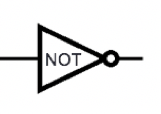
\includegraphics[height=0.5in]{../../resources/images/NOTx.png} \end{center}
\end{multicols}

%
 

{\bf Example digital circuit}: 

\begin{multicols}{2}
\begin{center}
   \includegraphics[width=1.2in]{../../resources/images/circuitEx.png} 
\end{center}
\columnbreak
Output when $x=1, y=0, z=0, w = 1$ is \underline{\phantom{$~~~0~~~$}}
Output when $x=1, y=1, z=1, w = 1$ is \underline{\phantom{$~~~0~~~$}}
Output when $x=0, y=0, z=0, w = 1$ is \underline{\phantom{$~~~0~~~$}}
\phantom{Output when $x=0, y=0, z=0, w = 0$ is \underline{\phantom{$~~~0~~~$}}}
\end{multicols}



Draw a logic circuit with inputs $x$ and $y$ whose output  is always $0$.  {\it  Can you use exactly 1 gate?}


\vspace{40pt} \newpage


{\bf Fixed-width addition}: adding one bit at time, using the usual column-by-column and carry arithmetic, and dropping the carry from the leftmost column so the result is the same width as the summands.  In many cases, this gives representation of the correct value for the sum when we interpret the summands
in fixed-width binary or in 2s complement.

For single column:
\begin{center}
\begin{tabular}{cc|cc}
\multicolumn{2}{c|}{Input}  & \multicolumn{2}{|c}{Output}  \\
$x_0$ & $y_0$ & $c_0$ & $s_0$  \\
\hline
$1$ & $1$ & \phantom{$1$} & \phantom{$0$} \\
$1$ & $0$ & \phantom{$0$} & \phantom{$1$}\\
$0$ & $1$ & \phantom{$0$} & \phantom{$1$}\\
$0$ & $0$ & \phantom{$0$} & \phantom{$0$}\\
\end{tabular}
\end{center}

\begin{center}
\includegraphics[width=1.5in]{../../resources/images/half-adder.png}
\end{center} \newpage


Draw a logic circuit that implements binary addition of 
two numbers that are each represented in fixed-width binary:
\begin{itemize}
\item Inputs  $x_0, y_0, x_1, y_1$ represent $(x_1  x_0)_{2,2}$ and $(y_1 y_0)_{2,2}$
\item Outputs  $z_0, z_1, z_2$ represent $(z_2  z_1 z_0)_{2,3} = (x_1  x_0)_{2,2} + (y_1 y_0)_{2,2}$ (may require up to width  $3$)
\end{itemize}

{\it First approach}: half-adder for each column, then combine carry from right column with sum of left column


Write expressions for the circuit output values in terms of input values:

$z_0 = \underline{\phantom{x_0 \oplus y_0\hspace{3in}}}$

$z_1 = \underline{\phantom{(x_1 \oplus y_1) \oplus c_0}\hspace{2.5in}}$ \phantom{where $c_0 = x_0 \land y_0$}

$z_2 = \underline{\phantom{(c_0 \land (x_1 \oplus y_1)) \oplus c_1}\hspace{2in}}$ \phantom{where $c_1 = x_1 \land y_1$}\\

\includegraphics[width=1.7in]{../../resources/images/width-2-adder.png}



{\it Second approach}: for middle column, first add carry from right column to $x_1$, then add result to $y_1$


Write expressions for the circuit output values in terms of input values:

$z_0 = \underline{\phantom{x_0 \oplus y_0}\hspace{3in}}$

$z_1 = \underline{ \phantom{(c_0 \oplus x_1) \oplus y_1}\hspace{2.4in}}$ \phantom{where $c_0 = x_0 \land y_0$}

$z_2 = \underline{\phantom{(c_0 \land x_1) \oplus ((c_0 \oplus x_1)\land y_1)}\hspace{1.5in}}$

\vfill

{\it Extra example} Describe how to generalize this addition circuit for larger width inputs.

 \newpage
\subsection*{Review: Week 2 Friday}
\begin{enumerate}
    \item {

\begin{enumerate}
    \item Consider the logic circuit
        \begin{center}
        \includegraphics[width=2in]{../../resources/images/review-circuit-1.png}
        \end{center}
        Calculate the value of the output of this circuit ($y_1$) for each of the following settings(s) of input values.
        \begin{enumerate}
            \item $x_1 = 1$, $x_2 = 1$
            \item $x_1 = 1$, $x_2 = 0$
            \item $x_1 = 0$, $x_2 = 1$
            \item $x_1 = 0$, $x_2 = 0$
        \end{enumerate}  \item Consider the logic circuit
        \begin{center}
        \includegraphics[width=2in]{../../resources/images/review-circuit-2.png}
        \end{center}
        For which of the following settings(s) of input values is the output
        $y_1 = 0$, $y_2 = 1$? (Select all and only those that apply.)
        \begin{enumerate}
            \item $x_1 = 0$, $x_2 = 0$, $x_3 = 0$, and $x_4 = 0$
            \item $x_1 = 1$, $x_2 = 1$, $x_3 = 1$, and $x_4 = 1$
            \item $x_1 = 1$, $x_2 = 0$, $x_3 = 0$, and $x_4 = 1$
            \item $x_1 = 0$, $x_2 = 0$, $x_3 = 1$, and $x_4 = 1$
        \end{enumerate}
      
    \end{enumerate}
     }
    \item {

Recall this circuit from class:
\begin{center}
    \includegraphics[width=1.2in]{../../resources/images/circuitEx.png} 
 \end{center}

 Which of the following is true about all possible 
 input values $x,y,z,w$? (Select all and only 
 choices that are true for all values.)
 \begin{enumerate}
    \item The output $out$ is set to $1$ exactly when $x$ is $0$,
    and it is set to $0$ otherwise.
    \item The output $out$ is set to $1$ exactly when  $(xyzw)_{2,4} < 8$,
    and it is set to $0$ otherwise.
    \item The output $out$ is set to $1$ exactly when  $(wzyx)_{2,4}$
    is an even integer,
    and it is set to $0$ otherwise.
 \end{enumerate} }
\end{enumerate}

\newpage

\section*{Monday October 11}


{\bf Logical operators} aka propositional connectives

\begin{tabular}{lccccp{4in}}
{\bf Conjunction} & AND & $\land$ &\verb|\land| & 2 inputs & Evaluates to $T$ exactly when {\bf both} inputs are $T$\\
{\bf Exclusive or} & XOR & $\oplus$ &\verb|\oplus| & 2 inputs & Evaluates to $T$ exactly when {\bf exactly one} of inputs is $T$\\
{\bf Disjunction} & OR & $\lor$ &\verb|\lor| & 2 inputs & Evaluates to $T$ exactly when {\bf at least one} of inputs is $T$\\
{\bf Negation} & NOT & $\lnot$ &\verb|\lnot| & 1 input & Evaluates to $T$ exactly when its input is $F$\\
\end{tabular} 

Truth tables: Input-output tables where we use $T$ for $1$ and $F$ for $0$.

\begin{center}
\begin{tabular}{cc||c|c|c}
\multicolumn{2}{c||}{Input}  & \multicolumn{3}{c}{Output} \\
& & {\bf Conjunction} &  {\bf Exclusive or} & {\bf Disjunction} \\
$p$ & $q$ & $p \land q$ &  $p  \oplus  q$ & $p \lor  q$ \\
\hline
$T$ & $T$ & $T$ & $F$ & $T$\\
$T$ & $F$ & $F$ & $T$ & $T$\\
$F$ & $T$ & $F$ & $T$ & $T$\\
$F$ & $F$ & $F$ & $F$ & $F$\\
\hline
& & \includegraphics[width=0.5in]{../../resources/images/xANDy.png}
&  \includegraphics[width=0.5in]{../../resources/images/xXORy.png}
&  \includegraphics[width=0.5in]{../../resources/images/xORy.png}
\end{tabular}
\qquad \qquad\qquad
\begin{tabular}{c||c}
Input & Output \\
& {\bf Negation} \\
$p$ & $\lnot p$ \\
\hline
$T$ & $F$ \\
$F$ & $T$\\
\hline & 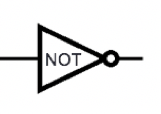
\includegraphics[width=0.5in]{../../resources/images/NOTx.png}
\end{tabular}
\end{center}
 

\begin{center}
    \begin{tabular}{ccc||p{3in}|c|c}
    \multicolumn{3}{c||}{Input}  & \multicolumn{3}{c}{Output} \\
    $p$ & $q$ & $r$  &  &  $(p \land q) \oplus (~ ( p \oplus q) \land r~)$ & $(p \land q) \vee (~ ( p \oplus q) \land r~)$ \\
    \hline
    $T$ & $T$  & $T$ &   && \\
    $T$ & $T$  & $F$ &   && \\
    $T$ & $F$  & $T$ &   && \\
    $T$ & $F$  & $F$ &   && \\
    $F$ & $T$  & $T$ &   && \\
    $F$ & $T$  & $F$ &   && \\
    $F$ & $F$  & $T$ &   && \\
    $F$ & $F$  & $F$ &   && \\
    \end{tabular}
\end{center}
    \vfill \newpage


Given a truth table, how do we find an expression
using the input variables and logical operators that has the 
output values specified in this table?

{\it Application}: design a circuit given a desired input-output relationship.

\begin{center}
\begin{tabular}{cc||cc}
\multicolumn{2}{c||}{Input}  &\multicolumn{2}{c}{Output}\\
$p$ & $q$& $mystery_1$ & $mystery_2$\\
\hline
$T$ & $T$  & $T$ & $F$\\
$T$ & $F$  & $T$ & $F$\\
$F$ & $T$  & $F$ & $F$\\
$F$ & $F$  & $T$ & $T$\\
\end{tabular}
\end{center}


Expressions that have output $mystery_1$ are

\vspace{100pt}

Expressions that have output $mystery_2$ are

\vspace{100pt}
 

{\bf  Definition} An expression built of variables and logical 
operators is in {\bf disjunctive normal form}  (DNF) means
that it is an OR of ANDs of variables and their negations.

{\bf  Definition} An expression built of variables and logical 
operators is in {\bf conjunctive normal form}  (CNF) means
that it is an AND of ORs of variables and their negations.
 



{\it Extra example}: An expression that has output ? is: 

\begin{tabular}{ccc||c}
    \multicolumn{3}{c||}{Input}  & Output\\
    $p$ & $q$ & $r$  &  ?\\
    \hline
    $T$ & $T$  & $T$ & $T$ \\
    $T$ & $T$  & $F$ & $T$ \\
    $T$ & $F$  & $T$ & $F$ \\
    $T$ & $F$  & $F$ & $T$ \\
    $F$ & $T$  & $T$ & $F$ \\
    $F$ & $T$  & $F$ & $F$ \\
    $F$ & $F$  & $T$ & $T$ \\
    $F$ & $F$  & $F$ & $F$ \\
\end{tabular}

\vfill

 \newpage
\subsection*{Review: Week 3 Monday}
\begin{enumerate}
    \item 

\begin{enumerate}
    \item Consider the logic circuit
    \begin{center}
    \includegraphics[width=2in]{../../resources/images/review-circuit-3.png}
    \end{center}
    For which of the following settings(s) of input values is the output
    $y_1 =  0$? (Select all and only those that apply.)
    \begin{enumerate}
        \item $x_1 = 0$, $x_2 = 0$, $x_3 = 0$, and $x_4 = 0$
        \item $x_1 = 1$, $x_2 = 1$, $x_3 = 1$, and $x_4 = 1$
        \item $x_1 = 1$, $x_2 = 0$, $x_3 = 0$, and $x_4 = 1$
        \item $x_1 = 0$, $x_2 = 0$, $x_3 = 1$, and $x_4 = 1$
    \end{enumerate}
    \item Consider the logic circuits
    \begin{center}
    \includegraphics[width=2in]{../../resources/images/review-circuit-1.png}
    \qquad \qquad \qquad
    \includegraphics[width=2in]{../../resources/images/review-circuit-4.png}
    \end{center}
    For which  of the following settings(s) of input values do the outputs
    of these  circuits have the  same value, i.e.\ $y_1 =  z_1$? 
    (Select all and only those that apply.)
    \begin{enumerate}
        \item $x_1 = 1$, $x_2 = 1$
        \item $x_1 = 1$, $x_2 = 0$
        \item $x_1 = 0$, $x_2 = 1$
        \item $x_1 = 0$, $x_2 = 0$
    \end{enumerate}    
    
\end{enumerate}     \item 

For each of the following compound propositions, determine
if it is in DNF, CNF, both, or neither.

\begin{enumerate}
    \item $(x \lor y \lor z) \land (x \land \lnot y \land z)$
    \item $\lnot (x \land y \land z) \land \lnot (\lnot x \land y \land \lnot z)$
\end{enumerate} \end{enumerate}
\newpage
\section*{Wednesday October 13}


{\bf Proposition}: Declarative sentence that is true or false (not both).

{\bf Propositional variable}: Variable that represents a proposition.

{\bf Compound proposition}: New proposition formed from existing propositions (potentially) using logical operators.
{\it Note}: A propositional variable is one example of a compound proposition.

{\bf Truth table}: Table with one row for each of the possible combinations of truth values of the input and 
    an additional column that shows the truth value of the result of the operation corresponding to a particular row.
    
 

{\bf Logical equivalence }: Two compound  propositions are {\bf logically  equivalent} means that  they 
have the  same  truth  values for all settings of truth  values to their propositional  variables.

{\bf Tautology}:  A compound proposition that evaluates to true
for all settings of truth  values to its propositional  variables; it is  abbreviated $T$.

{\bf Contradiction}: A compound proposition that  evaluates  to  false 
for  all settings of truth  values to its propositional  variables; it  is abbreviated $F$.

{\bf Contingency}: A compound proposition that is neither a tautology nor a contradiction.
 \vfill


Label each of the following as a tautology, contradiction, or contingency.

$p \land p$

$p \oplus p$

$p \lor p$

$p \lor \lnot p$

$p \land \lnot p$ \vfill


{\it Extra Example}: Which of the  compound propositions in the table below are logically equivalent?
\begin{center}
\begin{tabular}{cc||c|c|c|c|c}
\multicolumn{2}{c||}{Input}  & \multicolumn{5}{c}{Output} \\
$p$ & $q$ & $\lnot (p \land \lnot q)$ & $\lnot (\lnot p  \lor \lnot q)$ &  $(\lnot p \lor  q)$
& $(\lnot q \lor \lnot p)$ & $(p \land q)$  \\
\hline
$T$ & $T$ & &&&&\\
$T$ & $F$ & &&&&\\
$F$ & $T$ & &&&&\\
$F$ & $F$ & &&&&\\
\end{tabular}
\end{center} \vfill


\begin{center}
    \begin{tabular}{cc||c|c|c|c|c}
    \multicolumn{2}{c||}{Input}  & \multicolumn{5}{c}{Output} \\
     & & Conjunction &  Exclusive or & Disjunction  &  Conditional & Biconditional  \\
    $p$ & $q$ & $p \wedge q$ &  $p  \oplus  q$ & $p \vee  q$ & $p \to q$ & $p \leftrightarrow q$\\
    \hline
    $T$ & $T$ & $T$ & $F$ & $T$ & $T$& $T$\\
    $T$ & $F$ & $F$ & $T$ & $T$ & $F$& $F$\\
    $F$ & $T$ & $F$ & $T$ & $T$ & $T$& $F$\\
    $F$ & $F$ & $F$ & $F$ & $F$ & $T$& $T$\\
    \hline
    && ``$p$ and $q$'' & ``$p$ xor $q$'' & ``$p$ or $q$'' & ``if $p$ then $q$'' & ``$p$ if and only if $q$''
    \end{tabular}
\end{center}
     

The only way to make  the conditional statement $p \to q$ false is to \underline{\phantom{\hspace{3in}}}\\

\begin{tabular}{llll}
The {\bf  hypothesis}  of $p \to q$ is  &\underline{\phantom{\hspace{1in}}} &
The {\bf  antecedent}  of $p \to q$ is  &\underline{\phantom{\hspace{1in}}} \\
&&&  \\
The {\bf  conclusion}  of $p \to q$ is & \underline{\phantom{\hspace{1in}}}&
The {\bf  consequent}  of $p \to q$ is & \underline{\phantom{\hspace{1in}}}\\
&&&  \\
\end{tabular}
 

The {\bf converse}  of $p \to q$ is \underline{\phantom{ $q \to p$\hspace{1.6in}}}\\

The {\bf inverse}  of $p \to q$ is \underline{\phantom{ $\lnot p \to \lnot q$\hspace{1.6in}}}\\

The {\bf contrapositive}  of $p \to q$ is \underline{\phantom{$\lnot q \to \lnot p$\hspace{1.6in}}} \\
 \vfill


We can use a recursive definition to describe all 
compound propositions that use propositional variables 
from a specified collection.  Here's the definition
for all compound propositions whose propositional variables 
are in $\{p, q\}$.

\[
\begin{array}{ll}
\textrm{Basis Step: } & p \textrm{ and } q \textrm{ are each a compound proposition} \\
\textrm{Recursive Step: } & \textrm{If } x \textrm{ is a compound proposition then so is } (\lnot x) 
\textrm{ and if } \\
& x \textrm{ and } y \textrm{ are both compound propositions then so is each of }\\
&(x \land y), (x \oplus y), (x \lor y), (x \to y), (x \leftrightarrow y)
\end{array}
\] 

Order of operations (Precedence) for logical operators: 

Negation, then conjunction / disjunction, then conditional / biconditionals.

Example: $\lnot p \lor \lnot q$ means $(\lnot p) \lor (\lnot q)$.
 \newpage


{\bf (Some) logical equivalences}

{\it Can replace $p$ and $q$ with any compound proposition}

\begin{tabular}{llp{3in}}
$\lnot ( \lnot p) \equiv p$ & & {\bf Double negation}\\
&& \\
&& \\
$p \lor q \equiv q \lor p$ & $p \land q \equiv q \land p$ & {\bf Commutativity} Ordering of terms\\
&& \\
&& \\
$(p \lor q) \lor r  \equiv p \lor (q \lor r)$ & $(p \land q) \land r  \equiv p \land (q \land r)$ & {\bf Associativity} Grouping of terms\\
&& \\
&& \\
$p \land F \equiv F$ \qquad $p \lor T \equiv T$ & $p \land T \equiv p$ \qquad $p \lor F \equiv p$ & {\bf Domination} aka 
short circuit evaluation\\
&& \\
&& \\
$\lnot (p \land q) \equiv \lnot p \lor \lnot q$ & $\lnot (p \lor q) \equiv \lnot p \land\lnot q$  & {\bf DeMorgan's Laws}\\
&& \\
\end{tabular}

\begin{tabular}{llp{3in}}
$p \to q \equiv \lnot p \lor q$ & & \\
&& \\
&& \\
$p \to q \equiv \lnot q \to \lnot p$ & &{\bf Contrapositive} \\
&& \\
&& \\
$\lnot (p \to q) \equiv p\land \lnot q$  & &\\
&& \\
&& \\
$\lnot( p \leftrightarrow q) \equiv p \oplus q$ && \\
&& \\
&& \\
$p \leftrightarrow q \equiv q \leftrightarrow p$ &&\\
&& \\
\end{tabular}

{\it Extra examples}:

$p \leftrightarrow q$ is not logically equivalent to $p \land q$ because \underline{\phantom{\hspace{4in}}} 

$p \to q$ is not logically equivalent to $q \to p$ because \underline{\phantom{\hspace{4in}}} 
 \newpage
\subsection*{Review: Week 3 Wednesday}
\begin{enumerate}
    \item 

For each of the following propositions, indicate exactly one of:

\begin{itemize}
    \item There is no assignment of truth values to its variables that makes it true,
    \item There is exactly one assignment of truth values to its variables that makes it true, or
    \item There are exactly two assignments of truth values to its variables that make it true, or
    \item There are exactly three assignments of truth values to its variables that make it true, or
    \item \emph{All} assignments of truth values to its variables make it true.
\end{itemize}

\begin{enumerate}
    \item $x \land y \land (x \lor y)$
    \item $\lnot x \land y \land (x \lor y)$
    \item $x \land \lnot y \land (x \land y)$
    \item $\lnot x \land (y \lor \lnot y)$
    \item $x \land (y \lor \lnot x)$
\end{enumerate}     \item 

For each of the following propositions, indicate exactly one of:

\begin{itemize}
    \item There is no assignment of truth values to its variables that makes it true,
    \item There is exactly one assignment of truth values to its variables that makes it true, or
    \item There are exactly two assignments of truth values to its variables that make it true, or
    \item There are exactly three assignments of truth values to its variables that make it true, or
    \item \emph{All} assignments of truth values to its variables make it true.
\end{itemize}

\begin{enumerate}
    \item $(p \leftrightarrow q) \oplus (p \land q)$
    \item $(p \to q) \vee (q \to p)$
    \item $(p \to q) \land (q \to p)$
    \item $\lnot (p \to q) $
\end{enumerate} \end{enumerate}
\newpage
\section*{Friday October 15}


{\bf Common ways to express logical operators in English}:

{\bf Negation} $\lnot p$ can be said in English as 

\vspace{-20pt}
\begin{itemize}
\item Not $p$.
\item It's not the case that $p$.
\item $p$ is false.
\end{itemize}

{\bf Conjunction} $p \land q$ can be said in English as

\vspace{-20pt}
\begin{itemize}
    \item $p$ and $q$.
    \item Both $p$ and $q$ are true.
    \item $p$ but $q$.
\end{itemize}

{\bf Exclusive or} $p \oplus q$ can be said in English as

\vspace{-20pt}
\begin{itemize}
    \item $p$ or $q$, but not both.
    \item Exactly one of $p$ and $q$ is true.
\end{itemize}

{\bf Disjunction} $p \lor q$ can be said in English as

\vspace{-20pt}
\begin{itemize}
    \item $p$ or $q$, or both.
    \item $p$ or $q$ (inclusive).
    \item At least one of $p$ and $q$ is true.
\end{itemize}

{\bf Conditional} $p \to q$ can be said in English as

\begin{multicols}{2}
\begin{itemize}
    \item if $p$, then $q$.
    \item $p$ is sufficient for $q$.
    \item $q$ when $p$.
    \item $q$ whenever $p$.
    \item $p$ implies $q$.
    \item $q$ follows from $p$.
    \item $p$ is sufficient for $q$.
    \item $q$ is necessary for $p$.
    \item $p$ only if $q$.
\end{itemize}
\end{multicols}

{\bf Biconditional}

\vspace{-20pt}
\begin{itemize}
    \item $p$ if and only if $q$.
    \item $p$ iff $q$.
    \item If $p$ then $q$, and conversely.
    \item $p$ is necessary and sufficient for $q$.
\end{itemize} \newpage
\newpage


{\bf Translation}: Express each of the following sentences as compound propositions, using
the given propositions.

\begin{multicols}{2}
``A sufficient condition for the warranty to be good is that you bought the computer less than a year ago"
\columnbreak
\begin{align*}
w &\text{ is  ``the warranty is good"} \\
b &\text{ is  ``you bought the computer less than a year ago"} \\
\end{align*}
\end{multicols}
\vfill

\begin{multicols}{2}
``Whenever the message was sent from an unknown system, it is scanned for viruses."
\columnbreak
\begin{align*}
s &\text{ is  ``The message is scanned for viruses"} \\
u &\text{ is  ``The message was sent from an unknown system"} \\
\end{align*}
\end{multicols}
\vfill

\begin{multicols}{2}
``I will complete my to-do list only if I put a reminder in my calendar"
\columnbreak
\begin{align*}
d &\text{ is  ``I will complete my to-do list"} \\
c &\text{ is  ``I put a reminder in my calendar"} \\
\end{align*}
\end{multicols}
\vfill \newpage


{\bf Definition}: A collection of  compound  propositions
is called {\bf consistent} if  there
is  an assignment  of  truth values
to  the  propositional variables that makes
each of the compound propositions  true.
 

{\bf Consistency}: 
\begin{quote}
Whenever the system software is being upgraded, users cannot access the file system. 
If users can access the file system, then they can save new files. 
If users cannot save new files, then the system software is not being upgraded.
\end{quote}

\begin{enumerate}
\item Translate to symbolic compound propositions
\vfill
\item Look for some truth assignment to the propositional variables for which all the compound propositions output $T$
\vfill
\end{enumerate} \newpage
\subsection*{Review: Week 3 Friday}
\begin{enumerate}
    \item 

Express each of the following sentences as compound propositions, using
the given propositions.

\begin{enumerate}
\item ``If you try to run Zoom while your computer is running many applications,
the video is likely to be choppy and laggy." $t$ is ``you run Zoom while your
computer is running many applications'', $c$ is ``the video is likely to be choppy'',
$g$ is ``the video is likely to be laggy''
\begin{enumerate}
    \item $t \to (c \land g)$
    \item $(c \land g) \to t$
    \item $(c \land g) \leftrightarrow t$
    \item $t \oplus (c \land g)$
\end{enumerate}
\item ``To connect wirelessly on campus without logging in you need to use
the UCSD-Guest network."  $c$ is ``connect wirelessly 
on campus'', $g$ is ``logging in'', and $u$ is ``use UCSD-Guest network''.
\begin{enumerate}
    \item $c \land \lnot g \land u$
    \item $(c \land \lnot g) \lor u$
    \item $(c \land \lnot g) \oplus u$
    \item $(c \land \lnot g) \to u$
    \item $u \to (c \land \lnot g)$
    \item $u \leftrightarrow (c \land \lnot g)$
\end{enumerate}
\end{enumerate}
\vspace{20pt}     \item 

For each of  the following  system specifications, 
identify the compound propositions  that give their
translations to logic  and then determine if the
translated collection  of compound
propositions is consistent.

\begin{enumerate}
    \item Specification: If the computer is out of memory, then network connectivity is unreliable. No disk errors can occur when the computer is out of memory. Disk
    errors only occur when network connectivity is unreliable.
    
    Translation: $M =$ ``the computer is  out of memory"; $N = $ ``network connectivity
    is unreliable"; $D = $  ``disk errors  can occur".
    
    \begin{enumerate}
        \item \begin{align*} &\neg M \to  N  \\ & \neg D \to M \\ & D \to N \end{align*}
        \item \begin{align*} &M \to  \neg N  \\ & \neg D \wedge M \\ & N \to D \end{align*}
        \item \begin{align*} &M \to  N  \\ &  M \to \neg D \\ & \neg  N \to \neg D \end{align*}
    \end{enumerate}
    
    \newpage
    \item Specification: Whether you think you can, or you think you can't - you're right.
\footnote{Henry Ford}
    
    Translation: $T =$ ``you  think  you  can"; $C = $  ``you  can".
    
    \begin{enumerate}
        \item \begin{align*} &T \to C \\&  \neg T \to \neg C \end{align*}
        \item \begin{align*} &T \wedge C \\  & \neg  T \wedge \neg C \end{align*}
        \item \begin{align*} &T \to \neg T  \\ & C  \to \neg  C \end{align*}
    \end{enumerate}
    
    \item Specification: A secure password must be private and complicated. If
    a password is  complicated then  it will be hard to  remember.  People
    write down hard-to-remember passwords. If a password is written down, it's  not private.   The password is secure.

    Translation: $S =$ ``the password is secure"; $P = $ ``the password is private"; 
    $C = $  ``the password is  complicated"; $H = $ ``the password is hard to remember";
    $W =  $ ``the password is written down".
    
    \begin{enumerate}
        \item \begin{align*} &\neg (P \wedge C) \to \neg  S  \\ & C \to H  \\ & W \wedge H \\ & W \to  \neg P \\ & S \end{align*}
        \item \begin{align*} &(P \wedge  C)  \to S  \\ &  C \to H\\ & W  \to  H \\  & W \to P \\ & S\end{align*}
        \item \begin{align*} & S  \to (P \wedge C)  \\ &  C \to H\\ & H  \to  W \\  & W \to \neg P \\ & S\end{align*}
    \end{enumerate}

\end{enumerate} \end{enumerate}

\newpage 


\section*{Monday October 18}


Real-life representations are often prone to corruption.  Biological codes, like RNA, 
may mutate naturally\footnote{Mutations of specific RNA codons have been linked to many disorders and cancers.}
and during measurement; cosmic radiation and other ambient noise 
can flip bits in computer storage\footnote{This RadioLab podcast episode
goes into more detail on bit flips: \url{https://www.wnycstudios.org/story/bit-flip}}. 
One way to recover from corrupted data is to introduce or exploit redundancy. 

Consider the following algorithm to introduce redundancy in a string of $0$s and $1$s.
\begin{algorithm}[caption={Create redundancy by repeating each bit three times}]
procedure $\textit{redun3}$($a_{k-1} \cdots a_0$: a nonempty bitstring)
for $i$ := $0$ to $k-1$
  $c_{3i}$ := $a_i$
  $c_{3i+1}$ := $a_i$
  $c_{3i+2}$ := $a_i$
return $c_{3k-1} \cdots c_0$
\end{algorithm}

\begin{algorithm}[caption={Decode sequence of bits using majority rule on consecutive three bit sequences}]
procedure $\textit{decode3}$($c_{3k-1} \cdots c_0$: a nonempty bitstring whose length is an integer multiple of $3$)
for $i$ := $0$ to $k-1$
  if exactly two or three of $c_{3i}, c_{3i+1}, c_{3i+2}$ are set to $1$
    $a_i$ := 1
  else 
    $a_i$ := 0
return $a_{k-1} \cdots a_0$
\end{algorithm}

Give a recursive definition of the set of outputs of the $redun3$ procedure, $Out$,

\phantom{{\bf Basis step}: $000 \in Out$ and $111 \in Out$\\ {\bf Recursive step}: If $x \in Out$ then $x000 \in Out$ and $x111 \in Out$ (where $x000$ and $x111$ are the results of string concatenation).}


Consider the message $m = 0001$ so that the sender calculates $redun3(m) = redun3(0001) = 000000000111$.

Introduce $\underline{\phantom{~~4~~}} $
errors into the message so that the signal received by the 
receiver is $\underline{\phantom{010100010101}}$
but the receiver is still able to decode the original message.


{\it Challenge: what is the biggest number of errors you can introduce?} 

Building a circuit for lines 3-6 in $decode$ procedure: given three input bits, we need to determine whether the
majority is a $0$ or a $1$.

\begin{center}
\begin{multicols}{2}\begin{tabular}{ccc|c}
$c_{3i}$ & $c_{3i+1}$ & $c_{3i+2}$ & $a_i$ \\
\hline
$1$ & $1$ & $1$ & $\phantom{1}$ \\
$1$ & $1$ & $0$ & $\phantom{1}$ \\
$1$ & $0$ & $1$ & $\phantom{1}$ \\
$1$ & $0$ & $0$ & $\phantom{0}$ \\
$0$ & $1$ & $1$ & $\phantom{1}$ \\
$0$ & $1$ & $0$ & $\phantom{0}$ \\
$0$ & $0$ & $1$ & $\phantom{0}$ \\
$0$ & $0$ & $0$ & $\phantom{0}$ \\\\
\end{tabular}
\columnbreak

Circuit 
\end{multicols}
\end{center} \newpage


{\bf Definition}: The {\bf Cartesian product} of the sets $A$ and $B$, 
$A \times B$, is the set of all ordered pairs $(a, b)$, where $a \in A$ and $b \in B$. 
That is: $A \times B = \{(a, b) \mid (a \in A) \land (b \in B)\}$.
The Cartesian product of the sets $A_1, A_2, \ldots ,A_n$, denoted by 
$A_1 \times A_2 \times \cdots \times A_n$, is the
set of ordered n-tuples $(a_1, a_2,...,a_n)$, where $a_i$ belongs to 
$A_i$ for $i = 1, 2,\ldots,n$. That is,
\[
    A_1 \times A_2 \times \cdots \times A_n = \{(a_1, a_2,\ldots,a_n) \mid a_i \in A_i \textrm{ for } i = 1, 2,\ldots,n\}
\] 

Recall that $S$ is defined as the set of all RNA strands, nonempty strings made of the bases in 
$B = \{\A,\U,\G,\C\}$. 
We define the functions 
\[
  \textit{mutation}: S \times \mathbb{Z}^+ \times B \to S
\qquad \qquad
  \textit{insertion}: S \times \mathbb{Z}^+ \times B \to S
\]
\[
  \textit{deletion}: \{ s\in S \mid rnalen(s) > 1\} \times \mathbb{Z}^+ \to S
  \qquad \qquad \textrm{with rules}
\]

\begin{algorithm}
procedure $\textit{mutation}$($b_1\cdots b_n$: $\textrm{a RNA strand}$, $k$: $\textrm{a  positive integer}$, $b$: $\textrm{an  element of } B$)
for $i$ := $1$ to $n$
  if $i$ = $k$
    $c_i$ := $b$
  else
    $c_i$ := $b_i$
return $c_1\cdots c_n$ $\{ \textrm{The return value is a RNA strand made of the } c_i \textrm{ values}\}$
\end{algorithm}

\begin{algorithm}
procedure $\textit{insertion}$($b_1\cdots b_n$: $\textrm{a RNA strand}$, $k$: $\textrm{a  positive integer}$, $b$: $\textrm{an  element of } B$)
if $k > n$
  for $i$ := $1$ to $n$
    $c_i$ := $b_i$
  $c_{n+1}$ := $b$
else 
  for $i$ := $1$ to $k-1$
    $c_i$ := $b_i$
  $c_k$ := $b$
  for $i$ := $k+1$ to $n+1$
    $c_i$ := $b_{i-1}$
return $c_1\cdots c_{n+1}$ $\{ \textrm{The return value is a RNA strand made of the } c_i \textrm{ values}\}$
\end{algorithm}

\begin{algorithm}
procedure $\textit{deletion}$($b_1\cdots b_n$: $\textrm{a RNA strand with } n>1$, $k$: $\textrm{a  positive integer}$)
if $k > n$
  $m$ := $n$
  for $i$ := $1$ to $n$
    $c_i$ := $b_i$
else
  $m$ := $n-1$
  for $i$ := $1$ to $k-1$ 
    $c_i$ := $b_i$
  for $i$ := $k$ to $n-1$
    $c_i$ := $b_{i+1}$
return $c_1\cdots c_m$ $\{ \textrm{The return value is a RNA strand made of the } c_i \textrm{ values}\}$
\end{algorithm}
 

Trace the pseudocode to find the output of $\textit{mutation}(~ (\A\U\C, 3, \G) ~)$

\vspace{50pt}

Fill in the blanks so that $\textit{insertion}(~(\A\U\C, \underline{\phantom{3}}, \underline{\phantom{\G}})~) = \A\U\C\G$

\vspace{50pt}

Fill in the blanks so that $\textit{deletion}(~(\underline{\phantom{\G\G}}, \underline{\phantom{1}})~) =  \G$

\vspace{50pt}
 \newpage

\newpage
\subsection*{Review}
\begin{enumerate}
\item \hspace{1in}\\ 

In this question, we will consider how
to build a logic circuit with inputs $x_0$, $y_0$, $x_1$, $y_1$
and output $z$ such that $z = 1$ exactly when $(x_1x_0)_{2,2} < (y_1y_0)_{2,2}$ 
and $z = 0$ exactly when $(x_1x_0)_{2,2} \geq (y_1y_0)_{2,2}$.

\begin{enumerate}
    \item The first step towards designing this logic circuit is to construct its input-output table.
    How many rows does this table have (not including the header row labelling the columns)?
    \item What is the output for the row whose input values are $x_0 = 0$, $y_0 = 1$, $x_1 = 1$, $y_1 = 0$?
    \item What is the output for the row whose input values are $x_0 = 0$, $y_0 = 1$, $x_1 = 0$, $y_1 = 1$?
\end{enumerate}
 \item \hspace{1in}\\ 

Recall the procedures $redun3$ and $decode3$ from class.
\begin{enumerate}
\item  Give the output of $redun3(100)$.
\item  If the output of running $redun3$ is $000000111000111$, what was its input?
\item  Give the output of $decode3(100)$.
\item  How many distinct possible inputs to $decode3$ give the output $01$?
\end{enumerate} \item \hspace{1in}\\ 

Recall the procedures $mutation$ and $insertion$ and $deletion$ from class.
\begin{enumerate}
    \item Trace the pseudocode to find the output of $\textit{mutation}(~ (\A\U\C, 2, \U) ~)$
    \item Trace the pseudocode to find the output of $\textit{insertion}(~(\A\U\C, 1, \G)~)$
    \item Trace the pseudocode to find the output of $\textit{deletion}(~(\A\U\C, 1)~)$
\end{enumerate} \end{enumerate}

\newpage
\section*{Wednesday October 20}


{\bf  Definition}: A  {\bf predicate}  is  a function from a given set (domain) to $\{T,F\}$.

A predicate can be applied, or {\bf evaluated} at, an element of the domain.

Usually, a predicate {\it describes a  property} that domain elements may or may not have.

Two predicates over the same domain are {\bf equivalent} means they evaluate to
the same truth values for all possible assignments of domain elements to the
input. In other words, they are equivalent means that they are equal as functions.

To define a predicate, we must specify its domain and its value at each domain element.
The rule assigning truth values to domain elements can be specified using a formula, 
English description, in a table (if the domain is finite), or recursively (if the domain is recursively
defined). 

\begin{center}
    \begin{tabular}{c||c|c|c}
    Input & \multicolumn{3}{c}{Output} \\
    &$V(x)$ & $N(x)$ & $Mystery(x)$\\
    $x$ & $[x]_{2c,3} > 0$ & $[x]_{2c,3} < 0$& \\
    \hline
    $000$  & $F$ & & $T$\\
    $001$  & $T$ & & $T$\\
    $010$  & $T$ & & $T$\\
    $011$  & $T$ & & $F$\\
    $100$  & $F$ & & $F$\\
    $101$  & $F$ & & $T$\\
    $110$  & $F$ & & $F$\\
    $111$  & $F$ & & $T$\\
    \end{tabular}
    \end{center}
    
    The domain for each of the predicates $V(x)$, $N(x)$, $Mystery(x)$ is
    \underline{\phantom{$\{ b_1b_2b_3 ~\mid~ b_i \in \{0,1\} \textrm{ for each } i, 1 \leq i \leq 3 \}$}}.

    Fill in the table of values for the predicate $N(x)$ based on the formula given. \vfill


{\bf Definition}: The {\bf truth  set} of a  predicate is the collection of all elements in its
domain where the predicate evaluates to $T$.

Notice that specifying the domain and the truth set is sufficient for defining
a predicate. 

The truth set for the predicate $V(x)$ is $\underline{\phantom{\{ x ~\mid~ V(x) = T\} = \{ 001, 010, 011 \}}}$.

The truth set for the predicate $N(x)$ is $\underline{\phantom{\{ x ~\mid~ N(x) = T\} = \{ 101, 111 \}}}$.

The truth set for the predicate $Mystery(x)$ is $\underline{\phantom{\{ x ~\mid~ Mystery(x) = T\} = \{ 000, 001, 010, 101, 111 \}}}$.


\vfill \newpage


The {\bf universal quantification} of predicate $P(x)$ over
domain $U$ is the statement ``$P(x)$ for all values of $x$ in the domain $U$''
and is written $\forall x P(x)$ or $\forall x \in U ~P(x)$. 
When the domain is finite, universal quantification over the domain 
is equivalent to iterated {\it conjunction} (ands).

The {\bf existential quantification} of predicate $P(x)$ 
over domain $U$ is the statement ``There exists an element $x$ 
in the domain $U$ such that $P(x)$'' and is written $\exists x P(x)$
for $\exists x \in U ~P(x)$. 
When the domain is finite, existential quantification over the domain 
is equivalent to iterated {\it disjunction} (ors).

An element for which $P(x) = F$ is called a {\bf counterexample} of $\forall x P(x)$.

An element for which $P(x) = T$ is called a {\bf witness} of $\exists x P(x)$.
 

Statements involving predicates and quantifiers are {\bf logically equivalent} 
means they have the same truth value no matter which predicates (domains and functions) 
are substituted in. 

{\bf Quantifier version of De Morgan's laws}: 
$\boxed{\neg \forall x P(x) ~\equiv~ \exists x \left( \neg P(x) \right)}$
\qquad
\qquad
$\boxed{\neg \exists x Q(x) ~\equiv~ \forall x \left( \neg Q(x) \right)}$
 

Examples of quantifications using $V(x), N(x), Mystery(x)$:

{\bf True} or {\bf False}: $\exists x~ (~V(x) \land N(x)~)$

{\bf True} or {\bf False}: $\forall x~ (~V(x) \to N(x)~)$

{\bf True} or {\bf False}: $\exists x~ (~N(x) \leftrightarrow Mystery(x)~)$

Rewrite $\lnot \forall x~(~V(x) \oplus Mystery(x)~)$ into a logical equivalent statement.

\vspace{50pt}


Notice that these are examples where the predicates have {\it finite} domain.
How would we evaluate quantifications where the domain may be infinite? 

{\bf Example predicates on $S$, the set of RNA strands (an infinite set)}


$H: S \to \{T, F\}$ where $H(s) = T$ for all $s$.

Truth set of $H$ is \underline{\phantom{$S$\hspace{1in}}}\\

$F_{\A}: S \to \{T, F\}$  defined recursively by: 

~~Basis step: $F_{\A}(\A) = T$, $F_{\A}(\C) = F_{\A}(\G) = F_{\A}(\U) = F$

~~Recursive step: If $s \in S$ and $b \in B$, then $F_{\A}(sb) = F_{\A}(s)$.

Example where $F_{\A}$ evaluates to $T$ is \underline{\phantom{$\A\C\G$~\hspace{1in}}}

Example where $F_{\A}$ evaluates to $F$ is \underline{\phantom{$\U\A\C\U$\hspace{1in}}} \newpage
\subsection*{Review}
\begin{enumerate}
\item \hspace{1in}\\ 

Recall the predicates $V(x)$, $N(x)$, and $Mystery(x)$
on domain $\{000,001,010,011,100,101,110,111\}$ from class.
Which of the following is true? (Select  all and only that apply.)
 \begin{enumerate}
    \item $\left( \forall x ~V(x) \right) \lor \left( \forall x ~N(x) \right)$
    \item $\left( \exists x ~V(x) \right) \land \left( \exists x~N(x) \right) \land \left( \exists x~Mystery(x)\right)$
    \item $\exists x ~(~V(x) \land N(x) \land Mystery(x)~)$
    \item $\forall x ~(~V(x) \oplus N(x)~)$
    \item $\forall x ~(~Mystery(x) \to V(x)~)$
 \end{enumerate}    \item \hspace{1in}\\ 

Consider the following predicates, each of which has 
as its domain the set of all bitstrings whose leftmost bit is $1$

$E(x)$ is $T$ exactly when $(x)_{2}$ is even, and is $F$ otherwise

$L(x)$ is $T$ exactly when $(x)_2 < 3$, and is $F$ otherwise

$M(x)$ is $T$ exactly when $(x)_2 > 256$ and is $F$ otherwise.

\begin{enumerate}
\item What is $E(110)$?
\item Why is $L(00)$ undefined?
\begin{enumerate}
\item Because the domain of $L$ is infinite
\item Because $00$ does not have $1$ in the leftmost position
\item Because $00$ has length 2, not length 3
\item Because $(00)_{2,2} = 0$ which is less than $3$
\end{enumerate}
\item Is there a bitstring of width (where width is the number of bits) $6$ at which $M(x)$ evaluates 
to $T$?
\end{enumerate} \item \hspace{1in}\\ 

For this question, we will use the following predicate.

$F_{\A}$ with domain $S$ is defined recursively by: 
\begin{itemize}
\item[]Basis step: $F_{\A}(\A) = T$, $F_{\A}(\C) = F_{\A}(\G) = F_{\A}(\U) = F$
\item[]Recursive step: If $s \in S$ and $b \in B$, then $F_{\A}(sb) = F_{\A}(s)$
\end{itemize}

Which of the following is true? (Select  all and only that apply.)
 \begin{enumerate}
    \item $F_\A ( \A\A)$
    \item $F_\A ( \A\C)$
    \item $F_\A ( \A\G)$
    \item $F_\A ( \A\U)$
    \item $F_\A ( \C\A)$
    \item $F_\A ( \C\C)$
    \item $F_\A ( \C\G)$
    \item $F_\A ( \C\U)$
 \end{enumerate}    
 \end{enumerate}

\newpage
\section*{Friday October 22}


{\it Recall the definitions}: The set of RNA strands $S$ is defined (recursively) by:
\[
\begin{array}{ll}
\textrm{Basis Step: } & \A \in S, \C \in S, \U \in S, \G \in S \\
\textrm{Recursive Step: } & \textrm{If } s \in S\textrm{ and }b \in B \textrm{, then }sb \in S
\end{array}
\]
where $sb$ is string concatenation.

The function \textit{rnalen} that computes the length of RNA strands in $S$ is defined recursively by:
\[
\begin{array}{llll}
& & \textit{rnalen} : S & \to \mathbb{Z}^+ \\
\textrm{Basis Step:} & \textrm{If } b \in B\textrm{ then } & \textit{rnalen}(b) & = 1 \\
\textrm{Recursive Step:} & \textrm{If } s \in S\textrm{ and }b \in B\textrm{, then  } & \textit{rnalen}(sb) & = 1 + \textit{rnalen}(s)
\end{array}
\]

The function \textit{basecount} that computes the number of a given base 
$b$ appearing in a RNA strand $s$ is defined recursively by:
\[
\begin{array}{llll}
& & \textit{basecount} : S \times B & \to \mathbb{N} \\
\textrm{Basis Step:} &  \textrm{If } b_1 \in B, b_2 \in B & \textit{basecount}(~(b_1, b_2)~) & =
        \begin{cases}
            1 & \textrm{when } b_1 = b_2 \\
            0 & \textrm{when } b_1 \neq b_2 \\
        \end{cases} \\
\textrm{Recursive Step:} & \textrm{If } s \in S, b_1 \in B, b_2 \in B &\textit{basecount}(~(s b_1, b_2)~) & =
        \begin{cases}
            1 + \textit{basecount}(~(s, b_2)~) & \textrm{when } b_1 = b_2 \\
            \textit{basecount}(~(s, b_2)~) & \textrm{when } b_1 \neq b_2 \\
        \end{cases}
\end{array}
\] 

{\bf Using functions to define predicates}:

\fbox{\parbox{\textwidth}{
$L$ with domain $S \times \mathbb{Z}^+$ is defined by, for $s \in S$ and $n \in \mathbb{Z}^+$,
\[
L( ~(s, n)~) = \begin{cases}
T &\qquad\text{if $rnalen(s) = n$}\\
F &\qquad\text{otherwise}\\
\end{cases}
\]
In other words, $L(~(s,n)~)$ means $rnalen(s) = n$
}}

\fbox{\parbox{\textwidth}{
$BC$ with domain $S \times B \times \mathbb{N}$ is defined by, 
for $s \in S$ and $b \in B$ and $n \in \mathbb{N}$,
\[
BC(~(s, b, n)~) = \begin{cases}
T &\qquad\text{if $basecount(~(s,b)~) = n$}\\
F &\qquad\text{otherwise}\\
\end{cases}
\]
In other words, $BC(~(s,b,n)~)$ means $basecount(~(s,b)~) = n$
}}


Example where $L$ evaluates to $T$: $\underline{\phantom{(\A, 1)\hspace{1in}}}$  Why?

Example where $BC$ evaluates to $T$: $\underline{\phantom{(\A, \A1)\hspace{1in}}}$  Why?

Example where $L$ evaluates to $F$: $\underline{\phantom{(\A, 2)\hspace{1in}}}$ Why?

Example where $BC$ evaluates to $F$: $\underline{\phantom{(\A, \C, 1)\hspace{1in}}}$ Why? 

\fbox{\parbox{\textwidth}{
\[\exists t ~BC(t) \qquad \qquad 
\exists (s,b,n) \in S \times B \times \mathbb{N}~ (basecount(~(s,b)~) = n)\]

In English: \phantom{There exists an ordered $3$-tuple 
at which the predicate $BC$ evaluates to $T$.}

\vspace{30pt}

Witness that proves this existential quantification is true:\phantom{$(\G\G, \G, 2)$ or $(\G\A\U\G, \G, 2)$)}
}}

\fbox{\parbox{\textwidth}{
\[\forall t ~BC(t) \qquad \qquad 
\forall(s,b,n) \in S \times B \times \mathbb{N} ~(basecount(~(s,b)~) = n)\]

In English:\phantom{For all ordered $3$-tuples
the predicate $BC$ evaluates to $T$.}

\vspace{30pt}

Counterexample that proves this universal quantification is false: \phantom{$(\G\G, \A, 2)$ or $(\G\A\U\G, \G, 3)$)}
}}
 

{\bf New predicates from old}
\begin{enumerate}
\item Define the {\bf new} predicate with domain $S \times B$ and rule
\[
basecount(~(s,b)~) = 3
\]
Example domain element where predicate is $T$: \phantom{$(\A\U\A\A, \A)$}\\

\item Define the {\bf new} predicate with domain $S \times \mathbb{N}$ and rule
\[
basecount(~(s,\A)~) = n
\]
Example domain element where predicate is $T$: \phantom{$(\A\U\A,2)$}\\

\item Define the {\bf new} predicate with domain $S \times B$ and rule
\[
\exists n \in \mathbb{N} ~(basecount(~(s,b)~) = n)
\]
Example domain element where predicate is $T$: \phantom{$(\A\U\A,\A)$}\\

\item Define the {\bf new} predicate with domain $S$ and rule
\[
\forall b \in B ~(basecount(~(s,b)~) = 1)
\]
Example domain element where predicate is $T$: \phantom{$\A\C\G\U$}\\
\end{enumerate} 

{\bf Notation}: for a predicate $P$ with domain $X_1 \times \cdots \times X_n$ and a 
$n$-tuple $(x_1, \ldots, x_n)$ 
with each $x_i \in X$, we 
can write $P(x_1, \ldots, x_n)$ to mean $P( ~(x_1, \ldots, x_n)~)$.
 \newpage


{\bf Nested quantifiers}

\fbox{\parbox{\textwidth}{
\[
    \forall s \in S ~\forall b \in B ~\forall n \in \mathbb{N} ~(basecount(~(s,b)~) = n)
\]

In English: \phantom{There exists an ordered $3$-tuple 
at which the predicate $BC$ evaluates to $T$.}

\vspace{30pt}

Counterexample that proves this universal quantification is false:
\phantom{$(\G\G, \G, 3)$ or $(\G\A\U\G, \G, 2)$)}

\vspace{30pt}

}}

\fbox{\parbox{\textwidth}{
\[
    ~\forall n \in \mathbb{N} ~\forall s \in S ~\forall b \in B  ~(basecount(~(s,b)~) = n)
\]

In English: \phantom{There exists an ordered $3$-tuple 
at which the predicate $BC$ evaluates to $T$.}

\vspace{30pt}

Counterexample that proves this universal quantification is false:
\phantom{$(\G\G, \G, 3)$ or $(\G\A\U\G, \G, 2)$)}

\vspace{30pt}

}} 

{\bf Alternating nested quantifiers}

\fbox{\parbox{\textwidth}{
$$\forall s \in S ~\exists b\in B ~(~basecount(~(s,b)~) = 3~)$$

In English: For each RNA strand there is a base that occurs 3 times in this strand.\\

Write the negation and use De Morgan's law to find a 
logically equivalent version where the negation is applied only to the 
$BC$ predicate (not next to a quantifier).

\vspace{60pt}


Is the original statement {\bf True} or {\bf False}?

}}

\fbox{\parbox{\textwidth}{

$$\exists s \in S ~\forall b \in B ~\exists n \in \mathbb{N} ~(~basecount(~(s,b)~) = n~)$$

In English: There is an RNA strand so that for each base there is some nonnegative
integer that counts the number of occurrences of that base in this strand.\\

Write the negation and use De Morgan's law to find a 
logically equivalent version where the negation is applied only to the 
$BC$ predicate (not next to a quantifier).

\vspace{60pt}


Is the original statement {\bf True} or {\bf False}?

}}
 \newpage
\subsection*{Review}
\begin{enumerate}
\item \hspace{1in}\\

Recall the predicate $L$ with domain $S \times \mathbb{Z}^+$ from class,
$L(~(s,n)~)$ means $rnalen(s) = n$.
Which of the following is true? (Select  all and only that apply.)
\begin{enumerate}
   \item $\exists s \in S ~\exists n \in \mathbb{Z}^+ ~L(~(s,n)~)$
   \item $\exists s \in S ~\forall n \in \mathbb{Z}^+ ~L(~(s,n)~)$
   \item $\forall n \in \mathbb{Z}^+ ~\exists s \in S ~L(~(s,n)~)$
   \item $\forall s \in S ~\exists n \in \mathbb{Z}^+ ~L(~(s,n)~)$
   \item $\exists n \in \mathbb{Z}^+ ~\forall s \in S ~L(~(s,n)~)$
\end{enumerate} 
 \item \hspace{1in}\\

Recall the predicate $BC$ with domain $S \times B \times \mathbb{N}$ from class,
$BC(~(s,b,n)~)$ means $basecount(~(s,b)~) = n$.
Match each sentence to its English translation, or select none of the above.
\begin{enumerate}
\item $\forall s \in S ~\exists n \in \mathbb{N} ~\forall b \in B ~basecount(~(s,b)~) = n$
\item $\forall s \in S ~\forall b \in B ~\exists n \in \mathbb{N} ~basecount(~(s,b)~) = n$
\item $\forall s \in S ~\forall n \in \mathbb{N} ~\exists b \in B ~basecount(~(s,b)~) = n$
\item $\forall b \in B ~\forall n \in \mathbb{N} ~\exists s \in S ~basecount(~(s,b)~) = n$
\item $\forall n \in \mathbb{N} ~\forall b \in B ~\exists s \in S ~basecount(~(s,b)~) = n$
\end{enumerate}

\begin{enumerate}[label=\roman*.]
    \item For each RNA strand and each possible base, the number of that base in that strand is a nonnegative integer.
    \item For each RNA strand and each nonnegative integer, there is a base that occurs this many times in this strand.
    \item Every RNA strand has the same number of each base, and that number is a nonnegative integer.
    \item For every given nonnegative integer, there is a strand where each possible base appears the given number of times.
    \item For every given base and nonnegative integer, there is an RNA strand that has this base occurring this many times.
\end{enumerate}


{\it Challenge}: Express symbolically

\begin{quote}
    There are (at least) two different RNA strands that have the same number of $\A$s.
\end{quote} \end{enumerate}


\newpage

\section*{Monday October 25}
\subsection*{Proof strategies}


We now have propositional and predicate logic that can help us express 
statements about any domain. We will develop proof strategies to 
craft valid argument for proving that such statements are true or disproving
them (by showing they are false). We will practice these strategies with 
statements about sets and numbers, both because they are familiar and because they
can be used to build cryptographic systems. Then we will apply proof strategies
more broadly to prove statements about data structures and machine learning 
applications. 

When a predicate $P(x)$ is over a {\bf finite} domain:
\begin{itemize}
\item To show that $\forall x  P(x)$ is true: check that $P(x)$ evaluates to $T$ at each domain element by evaluating over and over.
\item To show that $\forall x  P(x)$ is false: find one counterexample, a domain element where $P(x)$ evaluates to $F$.
\item To show that $\exists x  P(x)$ is true: find one witness, a domain element where $P(x)$ evaluates to $T$.
\item To show that $\exists x  P(x)$ is false: check that $P(x)$ evaluates to $F$ at each domain element by evaluating over and over.
\end{itemize} 

\fbox{\parbox{\linewidth}{New! {\bf Proof of universal by exhaustion}: To prove that $\forall x \, P(x)$
is true when $P$ has a finite domain, evaluate the predicate at {\bf each} domain element to confirm that it is always T.
}} 

\fbox{\parbox{\linewidth}{

{\bf New! Proof by universal generalization}: To prove that $\forall x \, P(x)$
is true, we can take an arbitrary element $e$ from the domain of 
quantification and show that $P(e)$ is true, without making any assumptions about $e$ 
other than that it comes from the domain.


An {\bf arbitrary} element of a set or domain is a fixed but unknown element from that set. 
}}
 \newpage


{\bf Definitions}:

A {\bf set} is an  unordered collection of  elements.
When $A$ and  $B$ are sets,  $A = B$ (set equality) means  
\[
    \forall x  ( x\in A \leftrightarrow x \in B)
\]

When $A$ and  $B$ are sets, $A \subseteq B$ (``$A$ is a {\bf subset} of $B$") means 
\[
    \forall x  (x \in A  \to x  \in B)
\]

When $A$ and  $B$ are sets,  $A \subsetneq B$ (``$A$ is a {\bf proper subset} of $B$") means 
\[
    (A\subseteq B) \wedge  (A \neq B)
\] 

\fbox{\parbox{\linewidth}{

{\bf New! Proof of conditional by direct proof}: To prove that the conditional statement $p \to q$ is true, 
we can assume $p$ is true and use that assumption to show $q$ is true.
}}

\fbox{\parbox{\linewidth}{

{\bf New! Proof of conditional by contrapositive proof}: To prove that the implication $p \to q$ is true, 
we can assume $q$ is false and use that assumption to show $p$ is also false.
}}

\fbox{\parbox{\linewidth}{

{\bf New! Proof of disjuction using equivalent conditional}: To prove that the 
disjunction $p \lor q$ is true, we can rewrite it equivalently as $\lnot p \to q$ and
then use direct proof or contrapositive proof.
}} 

\fbox{\parbox{\linewidth}{{\bf New! Proof by Cases}: To prove $q$, we can 
work by cases by first describing all possible cases we might be in
and then showing that each one guarantees $q$.
Formally, if we know that $p_1 \lor p_2$ is true, 
and we can show that $(p_1 \to q)$ is true and we can show that $(p_2 \to q)$, 
then we can conclude $q$ is true.
}} 

\fbox{\parbox{\linewidth}{
{\bf New! Proof of conjunctions with subgoals}:
To show that $p \land q$ is true, we have two subgoals: subgoal (1) prove $p$ 
is  true; and, subgoal (2) prove $q$ is true.

\vspace{1em}

 To show that $p \land q$ is false, it's enough to prove that $\lnot p$.
 
 To show that $p \land q$ is false, it's enough to prove that $\lnot q$.
}} 

To prove that one set is a subset of another, e.g. to show $A \subseteq B$:

\vspace{50pt}

To prove that two sets are equal, e.g. to show $A = B$:

\vspace{50pt}
 

Example: $\{ 43, 7, 9 \} = \{ 7, 43, 9, 7\}$

\vspace{50pt}
 \newpage


{\bf Prove} or {\bf  disprove}: $\{ \A,  \C,  \U,  \G\} \subseteq \{ \A\A, \A\C, \A\U, \A\G \}$ 

\vspace{150pt}

{\bf Prove} or {\bf  disprove}: For some set $B$, $\emptyset \in B$.

\vspace{150pt}

{\bf Prove} or {\bf  disprove}: For every set $B$, $\emptyset \in B$.

\vspace{150pt}

{\bf Prove} or {\bf  disprove}: The empty set is a subset of every set.

\vspace{150pt}

{\bf Prove} or {\bf  disprove}: The empty set is a proper subset of every set.

\vspace{150pt}

{\bf Prove} or {\bf  disprove}: $\{ 4, 6 \} \subseteq \{ n \mid  \exists c \in \mathbb{Z} ( n = 4c) \} $

\vspace{150pt}

{\bf Prove} or {\bf  disprove}: $\{ 4, 6 \} \subseteq \{ n ~\textbf{mod}~10 \mid  \exists c \in \mathbb{Z} ( n = 4c) \} $

\vspace{150pt}

 \vfill


\fbox{\parbox{\textwidth}{

\vspace{10pt}

Consider \ldots, an {\bf arbitrary} \ldots.
{\bf Assume} \ldots, we {\bf want to show} that \ldots. Which is what was needed,
so the proof is complete $\square$.

\vspace{20pt} {\it or, in other words:} \vspace{20pt}

Let \ldots be an {\bf arbitrary} \ldots. {\bf Assume} \ldots, {\bf WTS} that \ldots {\bf QED}.

\vspace{10pt}

}} \newpage
\subsection*{Review}
\begin{enumerate}
\item \hspace{1in}\\ 

Suppose $P(x)$ is  a predicate over a domain $D$.
\begin{enumerate}
    \item True or False: To translate the statement
    ``There are at least two  elements in $D$
    where the predicate $P$ evaluates to true", we
    could  write
    \[
    \exists  x_1 \in D \, \exists x_2 \in D  \, (P(x_1) \wedge P(x_2))
    \]
    \item True or False: To translate the statement
    ``There are at most two  elements in $D$
    where the predicate $P$ evaluates to true", we
    could write
    \[
    \forall  x_1 \in D \, \forall x_2 \in D \, \forall x_3 \in  D \, \left(~ (~P(x_1) \wedge P(x_2)  \wedge P(x_3) ~) \to (~ x_1 = x_2 \vee x_2 = x_3 \vee x_1 = x_3~)~\right)
    \]
\end{enumerate} \item \hspace{1in}\\ 

For each of the following English statements, select
the correct translation, or select None.

{\it Challenge: determine which of the statements are true and which 
are false.}

\begin{enumerate}
\item Every set is a subset of itself.

\item Every set is an element of itself.

\item Some set is an element of all sets.

\item Some set is a subset of all sets.
\end{enumerate}

\begin{enumerate}
\item[i.] $\forall X ~\exists Y ~(X \in Y)$
\item[ii.] $\exists X ~\forall Y ~(X \in Y)$
\item[iii.] $\forall X ~\exists Y ~(X \subseteq Y)$
\item[iv.] $\exists X ~\forall Y ~(X \subseteq Y)$
\item[v.] $\forall X ~(X \in X)$
\item[vi.] $\forall X ~(X \subseteq X)$ 
\end{enumerate} \item We want to hear how the term and this class are going for you.
Please complete the midquarter feedback form: \href{https://forms.gle/w3D7ifAWnD5sWwHf9}{https://forms.gle/w3D7ifAWnD5sWwHf9}
\end{enumerate}

\newpage
\section*{Wednesday October 27}


{\bf Cartesian product}: When $A$ and  $B$ are sets, 
\[
    A \times  B = \{ (a,b) \mid a \in A  \wedge b  \in B \}
\]

Example: $\{43, 9\} \times  \{9, \mathbb{Z}\}  = $
    
Example: $\mathbb{Z} \times \emptyset  = $

{\bf Union}: When $A$ and  $B$ are sets,
\[
    A \cup  B = \{ x \mid x \in A  \vee x \in B \}
\]    
    
Example: $\{43, 9\} \cup \{9, \mathbb{Z}\}  = $

Example: $\mathbb{Z} \cup \emptyset  = $ 

{\bf Intersection}: When $A$ and  $B$ are sets,
\[
    A \cap  B = \{ x \mid x \in A  \wedge x \in B \}
\]    
Example: $\{43, 9\} \cap \{9,\mathbb{Z}\}  = $

Example: $\mathbb{Z} \cap \emptyset  = $


{\bf Set  difference}: When $A$ and  $B$ are sets,

\[
    A -  B = \{ x \mid x \in A  \wedge x \notin B \}
\]

Example: $\{43, 9\} - \{9, \mathbb{Z}\}  = $

Example: $\mathbb{Z} - \emptyset  = $

    
{\bf Disjoint sets}: sets $A$ and  $B$ are disjoint means $A \cap  B  = \emptyset$

Example: $\{43, 9\}, \{9, \mathbb{Z}\}$ are not  disjoint 

Example: The sets $\mathbb{Z}$ and $\emptyset$ are disjoint

    

{\bf Power set}: When $U$ is a set, $\mathcal{P}(U) = \{ X \mid X \subseteq U\}$

Example: $\mathcal{P}(\{43, 9\}) = $

Example: $\mathcal{P}(\emptyset) = $
 \newpage


Let $W =  \mathcal{P}(  \{ 1,2,3,4,5\} )$


Example elements in $W$ are:
\vspace{20pt}

{\bf Prove} or {\bf  disprove}:  $\forall  A \in W\,  \forall B \in W\,  \left( A \subseteq B
~\to ~ \mathcal{P}(A) \subseteq \mathcal{P}(B) \right)$

\vfill
\vfill
\vfill

{\it Extra example}: {\bf Prove} or {\bf  disprove}:  $\forall  A \in W\,  \forall B \in W\,  \left( \mathcal{P}(A)  =\mathcal{P}(B)
~\to ~ A = B \right)$

\vspace{20pt}

{\it Extra example}: {\bf Prove} or {\bf  disprove}:  $\forall  A \in W\,  \forall B \in W\, \forall C  \in W\,  \left( A\cup B  = A \cup  C
~\to ~ B = C \right)$

\vspace{20pt} \newpage
\subsection*{Review}
\begin{enumerate}
\item \hspace{1in}\\ 

Let $W =  \mathcal{P}(\{1,2,3,4,5\})$.
The statement $$\forall A \in W~ \forall B\in W~ \forall  C  \in W~  ( A \cup B =  A \cup C ~\to~  B = C) $$ is false.
Which of the following  choices for  $A, B, C$ could  
be used to  give a counterexample to this claim?
(Select all and only that  apply.)
\begin{enumerate}
    \item $A = \{ 1, 2, 3 \}, B = \{ 1, 2\}, C= \{1, 3\}$
    \item $A = \{ 1, 2, 3 \}, B = \{ 2\}, C= \{2\}$
    \item $A = \{ \emptyset, 1, 2, 3 \}, B = \{ 1, 2\}, C= \{1, 3\}$
    \item $A = \{ 1, 2, 3 \}, B = \{ 1, 2\}, C= \{1, 4\}$
    \item $A = \{ 1, 2 \}, B = \{ 2, 3\}, C= \{1, 3\}$
    \item $A = \{ 1,2 \}, B =  \{ 1,3\}, C =  \{ 1,3\}$
\end{enumerate} \item \hspace{1in}\\ 

Let $W =  \mathcal{P}(\{1,2,3,4,5\})$.
Consider the  statement
$$\forall A \in W~ \forall B\in W~  \big( ( \mathcal{P}(A) = \mathcal{P}(B) )~\to~ (A = B) \big) $$

This statement is true. A proof of this statement starts with universal generalization, c
onsidering
arbitrary $A$ and $B$ in $W$. At this point, it remains to prove that 
$( \mathcal{P}(A) = \mathcal{P}(B) )~\to~ (A = B)$
is true about these arbitrary elements.  There are two ways to proceed: 

\begin{itemize}
\item[] First approach: By direct proof, in which we assume the hypothesis of the 
conditional and work to show that the conclusion follows.
\item[] Second approach: By proving the contrapositive version of the conditional instead, in which we
assume the negation of the conclusion and work to show that the negation of hypothesis follows.
\end{itemize} 

\begin{enumerate}
    \item First approach, assumption.
    \item First approach, ``need to show".
    \item Second approach, assumption.
    \item Second approach, ``need to show".
\end{enumerate}

Pick an option from below for the assumption and ``need to show" in each approach.


\begin{multicols}{2}
\begin{enumerate}[label=(\roman*)]
\item $\forall X ( X \subseteq A \leftrightarrow X \subseteq B)$
\item $\exists X ( X \subseteq A \leftrightarrow X \subseteq B)$
\item $\forall X ( X \subseteq A \oplus X \subseteq B)$
\item $\exists X ( X \subseteq A \oplus X \subseteq B)$
\item $\forall x ( x \in A \leftrightarrow x \in B)$
\item $\exists x ( x \in A \leftrightarrow x \in B)$
\item $\forall x ( x \in A \oplus x \in B)$
\item $\exists x ( x \in A \oplus x \in B)$
\end{enumerate}
\end{multicols} \end{enumerate}

\newpage
\section*{Friday October 29}
\subsection*{Facts about numbers}


\begin{enumerate}
    \item Addition and multiplication of real 
    numbers are each commutative and associative. 
    \vspace{25pt}
    \item The product of two positive numbers is positive, of 
    two negative numbers is positive, and of a positive and a negative number is negative.
    \vspace{25pt}
    \item The sum of two integers, the product of two integers, and the 
    difference between two integers are each integers.
    \vspace{25pt}
    \item For every integer $x$ there is no integer strictly between $x$ and $x+1$, 
    \vspace{25pt}
    \item When $x, y$ are positive integers, $xy \geq x$ and $xy \geq y$.
    \vspace{25pt}
\end{enumerate}
 \subsection*{Factoring}


{\bf Definition}: When $a$ and $b$ are integers and $a$ is nonzero, 
{\bf $a$ divides $b$} means there is an integer $c$ such that $b = ac$ . 


Symbolically, $F(~(a,b)~) = \phantom{\exists c\in \mathbb{Z}~(b=ac)}$
and is  a predicate over the domain \underline{\phantom{$\mathbb{Z}^{\neq 0} \times \mathbb{Z}$}}


Other (synonymous) ways to say that $F(~(a,b)~)$ is true: 
\begin{center}
$a$ is a {\bf factor} of $b$
\qquad 
$a$ is a {\bf divisor} of $b$
\qquad  $b$ is a {\bf multiple} of $a$
\qquad
$a | b$
\end{center}

When $a$ is a positive integer and $b$ is any integer, $a | b$
exactly when $b \textbf{ mod } a = 0$

When $a$ is a positive integer and $b$ is any integer, $a | b$
exactly $b = a \cdot (b \textbf{ div } a)$ 

{\it Translate these quantified statements by matching to English statement on right.}

\begin{multicols}{2}
$\exists a\in \mathbb{Z}^{\neq 0} ~(~F(~(a,a)~)~)$

$\exists a\in \mathbb{Z}^{\neq 0} ~(~\lnot F(~(a,a)~)~)$

$\forall a\in \mathbb{Z}^{\neq 0} ~(~F(~(a,a)~)~)$

$\forall a\in \mathbb{Z}^{\neq 0} ~(~\lnot F(~(a,a)~)~)$


Every nonzero integer is a factor of itself.

No nonzero integer is a factor of itself.

At least one nonzero integer is a factor of itself.

Some nonzero integer is not a factor of itself.
\end{multicols} 

{\bf Claim}: Every nonzero integer is a factor of itself.

{\bf Proof}: 


\vspace{150pt}


{\bf Prove} or {\bf Disprove}: There is a nonzero integer that does not divide its square.



\vspace{150pt}

{\bf Prove} or {\bf Disprove}: Every positive factor of a positive integer is less than or equal to it.

\vspace{150pt}
 \newpage


{\bf Claim}: Every nonzero integer is a factor of itself and 
every nonzero integer divides its square.

\vspace{100pt}
 

{\bf Definition}: an integer $n$ is {\bf even} means that there is an integer $a$ such that $n = 2a$; 
an integer $n$ is {\bf odd} means that there is an integer $a$ such that $n = 2a+1$.  Equivalently, 
an integer $n$ is {\bf even} means $n ~\textbf{ mod }~2 = 0$; an integer $n$ is {\bf odd} means $n ~\textbf{ mod }~2 = 1$.  
Also, an integer is even if and only if it is not odd.
 

{\bf Definition}:  An integer $p$ greater than $1$ is called {\bf prime} means 
the only positive factors of 
$p$ are $1$ and $p$. A positive integer that is greater than $1$ and is not prime 
is called composite. 

{\it Extra examples}: Use the definition to prove that $1$ is not prime, $2$ is prime, $3$
is prime, $4$ is not prime, $5$ is prime, $6$ is not prime, and $7$ is prime.


{\bf True or False}: The statement ``There are three consecutive positive integers that are prime."

{\it Hint}: These numbers would be of the form $p, p+1, p+2$ (where $p$ is a positive integer).

{\bf Proof}: We need to show \underline{\phantom{$\exists p \in \mathbb{Z}^+ ~(~Pr(p) \land Pr(p+1) \land Pr(p+2)~)$}}

\vspace{200pt}

{\bf True or False}: The statement ``There are three consecutive odd positive integers that are prime."

{\it Hint}: These numbers would be of the form $p, p+2, p+4$ (where $p$ is an odd positive integer).

{\bf Proof}: We need to show \underline{\phantom{$\exists p \in \mathbb{Z}^+ ~(~(p \textbf{ mod } 2 = 1 \land Pr(p) \land Pr(p+2) \land Pr(p+4)~)$}}

\vspace{200pt}
 \newpage
\subsection*{Review}
\begin{enumerate}
    \item \hspace{1in}\\ 

Recall the predicate  $F(~(a,b)~)  = ``a \text{ is a factor of } b"$ over  
the domain $\mathbb{Z}^{\neq 0} \times \mathbb{Z}$ we worked with 
in class. Consider the following quantified
statements
\begin{multicols}{2}
\begin{enumerate}[label=(\roman*)]
\item $\forall x \in \mathbb{Z} ~(F(~(1,x)~))$
\item $\forall x \in \mathbb{Z}^{\neq 0} ~(F(~(x,1)~))$
\item $\exists x \in \mathbb{Z} ~(F(~(1,x)~))$
\item $\exists x \in \mathbb{Z}^{\neq 0} ~(F(~(x,1)~))$
\item $\forall x \in \mathbb{Z}^{\neq 0} ~\exists y \in \mathbb{Z} ~(F(~(x,y)~))$
\item $\exists x \in \mathbb{Z}^{\neq 0} ~\forall y \in \mathbb{Z} ~(F(~(x,y)~))$
\item $\forall y \in \mathbb{Z} ~\exists x \in \mathbb{Z}^{\neq 0} ~(F(~(x,y)~))$
\item $\exists y \in \mathbb{Z} ~\forall x \in \mathbb{Z}^{\neq 0} ~(F(~(x,y)~))$
\end{enumerate}
\end{multicols}
\begin{enumerate}
\item Select the statement whose translation is
\begin{quote}
``The number $1$ is  a factor of every integer."
\end{quote}
or write NONE if none of (i)-(viii) work.

\item Select the statement whose translation is
\begin{quote}
``Every integer has at least one nonzero factor."
\end{quote}
or write NONE if none of (i)-(viii) work.

\item Select the statement whose translation is
\begin{quote}
``There is an integer of which
all nonzero integers are a factor."
\end{quote}
or write NONE if none of (i)-(viii) work.

\item For each  statement (i)-(viii), determine
if  it is true or  false.
\end{enumerate}     \item \hspace{1in}\\ 

Which of the following formalizes the definition of the predicate
$Pr(x)$ over the set of integers, and evaluates to $T$ exactly when 
$x$ is prime. (Select all and only correct options.)

\begin{enumerate}
    \item $\forall a \in \mathbb{Z}^{\neq 0}~( ~(x > 1 \land a >0) \to F(~(a,x)~))$
    \item $\lnot \exists a \in \mathbb{Z}^{\neq 0} ~(x > 1 \land (a=1 \lor a=x) \land F(~(a,x)~))$
    \item $(x > 1) \land \forall a \in \mathbb{Z}^{\neq 0}~( ~(~ a>0 \land F(~(a,x)~)~) \to (a=1 \lor a=x)~)$
    \item $(x > 1) \land \forall a \in \mathbb{Z}^{\neq 0}~( ~(~ a>1 \land \lnot (a=x) ~) \to \lnot F(~(a,x)~)~)$
\end{enumerate} \end{enumerate}


\newpage

\section*{Monday November 1}

Today's session is on Zoom, log in with your @ucsd.edu account https://ucsd.zoom.us/j/97431852722
Meeting ID: 974 3185 2722



{\it Recall the definitions}: The set of RNA strands $S$ is defined (recursively) by:
\[
\begin{array}{ll}
\textrm{Basis Step: } & \A \in S, \C \in S, \U \in S, \G \in S \\
\textrm{Recursive Step: } & \textrm{If } s \in S\textrm{ and }b \in B \textrm{, then }sb \in S
\end{array}
\]
where $sb$ is string concatenation.

The function \textit{rnalen} that computes the length of RNA strands in $S$ is defined recursively by:
\[
\begin{array}{llll}
& & \textit{rnalen} : S & \to \mathbb{Z}^+ \\
\textrm{Basis Step:} & \textrm{If } b \in B\textrm{ then } & \textit{rnalen}(b) & = 1 \\
\textrm{Recursive Step:} & \textrm{If } s \in S\textrm{ and }b \in B\textrm{, then  } & \textit{rnalen}(sb) & = 1 + \textit{rnalen}(s)
\end{array}
\]

The function \textit{basecount} that computes the number of a given base 
$b$ appearing in a RNA strand $s$ is defined recursively by:
\[
\begin{array}{llll}
& & \textit{basecount} : S \times B & \to \mathbb{N} \\
\textrm{Basis Step:} &  \textrm{If } b_1 \in B, b_2 \in B & \textit{basecount}(~(b_1, b_2)~) & =
        \begin{cases}
            1 & \textrm{when } b_1 = b_2 \\
            0 & \textrm{when } b_1 \neq b_2 \\
        \end{cases} \\
\textrm{Recursive Step:} & \textrm{If } s \in S, b_1 \in B, b_2 \in B &\textit{basecount}(~(s b_1, b_2)~) & =
        \begin{cases}
            1 + \textit{basecount}(~(s, b_2)~) & \textrm{when } b_1 = b_2 \\
            \textit{basecount}(~(s, b_2)~) & \textrm{when } b_1 \neq b_2 \\
        \end{cases}
\end{array}
\] 
At this point, we've seen the proof strategies
\begin{multicols}{2}
    \begin{itemize}
        \item A {\bf counterexample} to prove that  $\forall x P(x)$ is {\bf false}.
        \item  A {\bf witness} to prove that  $\exists x P(x)$ is {\bf true}.
        \item {\bf Proof of universal by exhaustion} to prove that $\forall x \, P(x)$
    is true when $P$ has a finite domain
        \item  {\bf Proof by universal generalization} to prove that $\forall x \, P(x)$
    is true using an arbitrary element of the domain.
        \item To  prove  that $\exists x P(x)$ is {\bf false}, write the universal statement that is 
        logically equivalent to its negation and then prove it true using universal generalization.
        \item To prove that $p \land q$ is true, have two subgoals: 
        subgoal (1) prove $p$ is  true; and, subgoal (2) prove $q$ is true. To prove that $p \land q$ is false, it's enough to prove that $p$ is false.
     To prove that $p \land q$ is false, it's enough to prove that $q$ is false.
        \item Proof of conditional by {\bf direct proof}
        \item Proof of conditional by {\bf contrapositive proof}
        \item Proof of disjuction using equivalent conditional: To prove that the 
        disjunction $p \lor q$ is true, we can rewrite it equivalently as $\lnot p \to q$ and
        then use direct proof or contrapositive proof.
        \item {\bf Proof by cases}.
    \end{itemize}
\end{multicols}
\newpage


Which proof strategies could be used to prove each of the following statements?

{\it Hint: first translate the statements to English and identify the main logical structure.}

$\forall s \in S~(~rnalen(s) > 0~)$

\vspace{100pt}

$\forall b \in B~\exists s \in S~(~basecount(~(s,b)~)~ > 0~)$

\vspace{100pt}

$\forall s \in S ~\exists b\in B ~(~basecount(~(s,b)~) > 0~)$

\vspace{100pt}

$\exists s \in S \, (\textit{rnalen(s)} = \textit{basecount}(~(s, \A)~)$

\vspace{100pt}

$\forall s \in S \, (\textit{rnalen(s)} \geq \textit{basecount}(~(s, \A)~))$

\vspace{100pt}

 \newpage


{\bf Claim} $\forall s \in S ~(~rnalen(s) > 0~)$

{\bf Proof}: Let $s$ be an arbitrary RNA strand. By the recursive definition of $S$,
either $s \in B$ or there is some strand $s_0$ and some base $b$ such that $s = s_0 b$.
We will show that the inequality holds for both cases.

{$\phantom{Basis}$} {\bf Case}: Assume $s \in B$. We need to show $rnalen(s) > 0$. 
By the basis step in the definition of $rnalen$,
$$rnalen(s) = 1$$
which is greater than $0$, as required.

{$\phantom{Recursive}$} {\bf Case}: Assume there is some strand $s_0$ and some base $b$ 
such that $s = s_0 b$. We will show {\it (the stronger claim)} that 
\[
    \forall u \in S ~\forall b \in B ~( ~\textit{rnalen}(u) >0  \to 
    \textit{rnalen}(ub) >0 ~)
\]
Consider an arbitrary RNA strand $u$ and an arbitrary base $b$, and assume towards a
direct proof,$~~{\phantom{ this is the induction hypothesis}}~~$ that
\[
    rnalen(u) > 0
\]
We need to show that $rnalen(ub) > 0$.
\[
    rnalen(ub) = 1 + rnalen (u) > 1 + 0 = 1 > 0
\]
as required. 

\fbox{\parbox{\textwidth}{{\bf Proof by Structural Induction} 
To prove a universal quantification over a recursively defined set:
\begin{itemize}
    \item[] {\bf Basis Step}:  Show the statement holds for elements specified in the basis step of the definition.
    \item[]  {\bf Recursive Step}:  Show that if the statement is true for each of the elements used to construct
    new elements in the recursive step of the definition, the result holds for these new elements.
    \end{itemize}
}}
     \newpage


{\bf Claim} $\forall s \in S \, (\textit{rnalen(s)} \geq \textit{basecount}(~(s, \A)~))$:

{\bf Proof}: We proceed by structural induction on the recursively defined set $S$.

{\bf Basis  Case}: We need to prove that 
the inequality holds for each element in the basis step of the recursive
definition of $S$. 
Need to show 
\begin{align*}
          &(~ rnalen(\A) \geq basecount(~(\A, \A)~)~) \land (~ rnalen(\C) \geq basecount(~(\C, \A)~)~) \\
    \land & (~ rnalen(\U) \geq basecount(~(\U, \A)~)~) \land (~ rnalen(\G) \geq basecount(~(\G, \A)~)~)
\end{align*}
We calculate, using the definitions of $rnalen$ and $basecount$:

\vspace{100pt}

{\bf Recursive Case}: We will prove that 
\[
    \forall u \in S ~\forall b \in B ~( ~rnalen(u) \geq basecount(~(u, \A)~) \to 
    rnalen(ub) \geq basecount(~(ub, \A)~)
\]

Consider arbitrary RNA strand $u$ and arbitrary base $b$. Assume, as the {\bf induction hypothesis},
that $rnalen(u) \geq basecount(~(u,\A)~)$. We need to show that $rnalen(ub) \geq basecount(~(ub, \A)~)$.

Using the recursive step in the definition of the function $rnalen$:
\[
    rnalen(ub) = 1 + rnalen(u)
\]
The recursive step in the definition of the function $basecount$ has two cases. We notice that 
$b = \A \lor b \neq \A$ and we proceed by cases.

{\it Case i.} Assume $b = \A$.

Using the first case in the recursive step in the definition of the function $basecount$:
\[
    basecount(~(ub, \A)~) = 1 + basecount(~(u,\A)~)
\]
By the {\bf induction hypothesis}, we know that $basecount(~(u,\A)~) \leq rnalen(u)$ so:
\[
    basecount(~(ub, \A)~) = 1 + basecount(~(u,\A)~) \leq 1 + rnalen(u) = rnalen (ub)
\]
and, thus, $basecount(~(ub,\A)~) \leq rnalen(ub)$, as required.

{\it Case ii.} Assume $b \neq \A$. 

Using the second case in the recursive step in the definition of the function $basecount$:
\[
    basecount(~(ub, \A)~) = basecount(~(u,\A)~)
\]
By the {\bf induction hypothesis}, we know that $basecount(~(u,\A)~) \leq rnalen(u)$ so:
\[
    basecount(~(ub, \A)~) = basecount(~(u,\A)~) \leq rnalen(u) < 1 + rnalen(u) = rnalen (ub)
\]
and, thus, $basecount(~(ub,\A)~) \leq rnalen(ub)$, as required.
 \newpage
\subsection*{Review}


Recall the definitions of the functions $rnalen$ and $basecount$ from class.

\begin{enumerate}
    \item Select all and only options that give a witness for the existential quantification
    $$\exists s \in S ~(~rnalen(s) = basecount(~(s,\U)~)~)$$
    \begin{enumerate}
    \item $\A$
    \item $\U\U$
    \item $\C\U$
    \item $(\U, 1)$
    \item None of the above.
    \end{enumerate}
    
    \item Select all and only options that give a counterexample for the universal quantification
    $$\forall s \in S ~(~rnalen(s) > basecount(~(s,\G)~)~)$$
    \begin{enumerate}
    \item $\U$
    \item $\G\G$
    \item $\A\G$
    \item $\C\U\G$
    \item None of the above.
    \end{enumerate}
    
    \item Select all and only the true statements
    \begin{enumerate}
    \item $\forall s \in S ~\exists b \in B ~\left(~rnalen(s) = basecount(~(s,b)~)~ \right)$
    \item $\exists s \in S ~\forall b \in B ~\left(~rnalen(s) = basecount(~(s,b)~)~ \right)$
    \item \begin{align*} \forall s_1 \in S~\forall s_2 \in S ~&\forall b \in B ~\big( ~\big( rnalen(s_1) = basecount(~(s_1,b)~) \\
    &\land rnalen(s_2) = basecount(~(s_2,b)~) \land rnalen(s_1) = rnalen(s_2) \big) \to s_1 = s_2  \big)\end{align*}
    \item None of the above.
    \end{enumerate}
    
\end{enumerate} 
\newpage
\section*{Wednesday November 3}


To organize our proofs, it's useful to highlight which claims are most important for 
our overall goals.
We use some terminology to describe different roles statements can have.

{\bf Theorem}: Statement that can be shown to be true, usually an important one.

Less important theorems can be called {\bf proposition}, {\bf fact}, {\bf result}, {\bf claim}.

{\bf Lemma}: A less important theorem that is useful in proving a theorem.
 
{\bf Corollary}: A theorem that can be proved directly after another one has been proved, 
without needing a lot of extra work.

{\bf Invariant}: A theorem that describes a property that is true about an algorithm or 
system no matter what inputs are used.




 

\begin{center}
    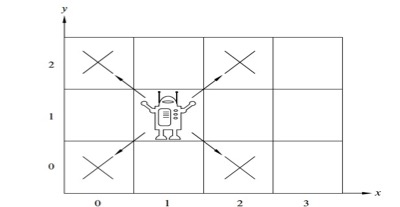
\includegraphics[width=3in]{../../resources/images/robot-grid.png}
\end{center}
    
{\bf Theorem}: A robot on an infinite 2-dimensional integer grid starts at $(0,0)$ and at each step moves
to diagonally adjacent grid point. This robot can / cannot {\footnotesize({\it circle one})} reach $(1,0)$.


{\bf Definition} The set of positions the robot can visit  $P$ is defined by:
\[
\begin{array}{ll}
    \textrm{Basis Step: } & (0,0) \in P \\
    \textrm{Recursive Step: } & \textrm{If } (x,y) \in P  \textrm{, then } 
    \phantom{(x+1, y+1), (x+1, y-1), (x-1, y-1), (x-1, y+1)} \textrm{ are also in } P
\end{array}
\]

{\it Example elements of $P$ are}:
\vspace{40pt}

{\bf Lemma}: $\forall (x,y) \in P( x+y \textrm{ is an even integer}~)$

{\it Why are we calling this a lemma?}


Proof of theorem using lemma: To show is $(1,0) \notin P$. Rewriting the lemma to explicitly 
restrict the domain of the universal, 
we have $\forall (x,y) ~(~ (x,y) \in P  \to (x+y \textrm{ is an even integer})~)$.  Since
the universal is true, 
$ (~ (1,0) \in P \to (1+0 \textrm{ is an even integer})~)$ is a true statement.
Evaluating the conclusion of this conditional statement: 
By definition of long division, since $1 = 0 \cdot 2 + 1$ (where $0 \in \mathbb{Z}$ and 
$1 \in \mathbb{Z}$ and $0 \leq 1 < 2$ mean that $0$ is the quotient and $1$ is the remainder), $1 ~\textrm{\bf mod}~ 2 = 1$ which is not $0$ 
so the conclusion is false.  A true conditional with a false conclusion must have a false hypothesis.
Thus, $(1,0) \notin P$, QED. $\square$

\vspace{20pt}

Proof of lemma by structural induction:

{\bf Basis Step}:

\vspace{100pt}


{\bf Recursive Step}:  Consider arbitrary $(x,y) \in P$.  To show is:
\[
(x+y \text{ is an even integer}) \to (\text{sum of coordinates of next position is even integer})
\]
Assume {\bf as the induction hypothesis, IH} that: 


\vspace{400pt} \newpage


The set $\mathbb{N}$ is recursively defined.
Therefore, the function $sumPow: \mathbb{N} \to \mathbb{N}$
which computes, for input $i$, the sum of the nonnegative powers of $2$
up to and including exponent $i$ is defined
recursively by

\begin{alignat*}{2}
    \text{Basis step:  } \qquad & sumPow(0) = 1 &\\
    \text{Recursive step:  } & \text{If } x \in \mathbb{N} \text{, then } &sumPow(x+1) = sumPow(x) + 2^{x+1}
\end{alignat*}

$sumPow(0) =$

\vspace{20pt}

$sumPow(1) =$

\vspace{20pt}

$sumPow(2) =$

\vspace{20pt}


Fill in the blanks in the following proof of 
\[
    \forall n \in \mathbb{N}~(sumPow(n) = 2^{n+1} - 1)
\]

{\bf Proof}: Since $\mathbb{N}$ is recursively defined, we proceed by \underline{\phantom{structural induction \hspace{0.3in}}}.

{\bf Basis case}: We need to show that \underline{\phantom{$sumPow(0) = 2^{0+1} - 1$ \hspace{0.2in}}}.
Evaluating each side: $LHS = sumPow(0) = 1$ by the basis case in the recursive definition
of $sumPow$; $RHS = 2^{0+1} - 1 = 2^1 - 1 = 2-1 = 1$. Since $1=1$, the equality holds.

{\bf Recursive case}: Consider arbitrary natural number $n$ and assume, as the 
\underline{\phantom{Induction Hypothesis (IH)}} that $sumPow(n) = 2^{n+1} - 1$. We need to show that
\underline{\phantom{$sumPow(n+1) = 2^{(n+1) + 1} - 1$}}.  Evaluating each side: 
\[
LHS = sumPow(n+1) \overset{\text{rec def}}{=} sumPow(n)  + 2^{n+1}\overset{\text{IH}}{=} (2^{n+1} - 1) + 2^{n+1}.
\]
\[
RHS = 2^{(n+1)+1}- 1 \overset{\text{exponent rules}}{=} 2 \cdot 2^{n+1} -1  = \left(2^{n+1} + 2^{n+1} \right) - 1
\overset{\text{regrouping}}{=}  (2^{n+1} - 1) + 2^{n+1} 
\]
Thus, $LHS = RHS$. The structural induction is complete and we have proved the universal generalization.
$\square$

 \vfill


\fbox{\parbox{\textwidth}{

{\bf Proof by Mathematical Induction}

To prove a universal quantification over the set of all integers greater than
or  equal to some  base integer $b$,

\vspace{-10pt}

\begin{itemize}
\item[] {\bf Basis Step}:  Show the property holds for $b$. 
\item[]  {\bf Recursive Step}:  Consider an arbitrary integer $n$ greater than or  equal to  $b$, assume
    (as the {\bf induction hypothesis})  that the property holds  for $n$, and use  this and
    other facts to  prove that  the property holds for $n+1$.
\end{itemize}

}} \newpage
\subsection*{Review}
\begin{enumerate}
\item \hspace{1in}\\ 

Recall the set $P$ defined by the recursive definition
\[
\begin{array}{ll}
    \textrm{Basis Step: } & (0,0) \in P\\
     \textrm{Recursive Step: } & \textrm{If } (x,y) \in P \textrm{ then } 
     (x+1, y+1) \in P \textrm{ and } (x+1, y-1) \in P \textrm{ and }\\ 
     & (x-1,y-1) \in P 
     \textrm{ and } (x-1, y+1) \in P
\end{array}
\]
\begin{enumerate}
\item Select all and only the ordered pairs below that are elements of $P$
\begin{enumerate}
\item $(0,0)$
\item $(4,0)$
\item $(1,1)$
\item $(1.5,2.5)$
\item $(0, -2)$
\end{enumerate}
\item What is another description of the set $P$ ? (Select all and only the true descriptions.)
\begin{enumerate}
\item $\mathbb{Z} \times \mathbb{Z}$
\item $\{ (n,n) ~|~ n \in \mathbb{Z} \}$
\item $\{ (a,b) \in \mathbb{Z} \times \mathbb{Z} ~|~ (a+b) \textbf{ mod } 2 =0 \}$
\end{enumerate}
\end{enumerate} \item \hspace{1in}\\ 

Select all and only the true statements below about the relationship between
structural induction and mathematical induction.
\begin{enumerate}
    \item Both structural induction and mathematical induction are proof strategies that 
    may be useful when proving universal claims about recursively defined sets.
    \item Mathematical induction is a special case of structural induction, for the case when 
    the domain of quantification is $\{ n \in \mathbb{Z} \mid n \geq b\}$ for some integer $b$.
    \item Universal claims about the set of all integers may be proved using structural induction
    but not using mathematical induction.
\end{enumerate} \newpage
\item \hspace{1in}\\ 

Consider the following function definitions
\[
    2^n: \mathbb{N} \to \mathbb{N} \text{ given by } 2^0 = 1 ~~\text{ and }~~
    2^{n+1} = 2 \cdot 2^n  
\]
\[
    n!: \mathbb{N} \to \mathbb{N} \text{ given by } 0! = 1 ~~\text{ and }~~
    (n+1)! = (n+1) n!
\]
\begin{enumerate}
\item Select all and only true statements below: 
    \begin{enumerate}
        \item $2^0 < 0!$
        \item $2^1 < 1!$
        \item $2^2 < 2!$
        \item $2^3 < 3!$
        \item $2^4 < 4!$
        \item $2^5 < 5!$
        \item $2^6 < 6!$
        \item $2^7 < 7!$
    \end{enumerate}

\item Fill in the blanks in the following proof.

{\bf Claim}: For all integers $n$ greater than or equal to $4$, $2^n < n!$ \\

{\bf Proof}: We proceed by mathematical induction on the set of integers greater than or equal to $4$.

{\bf Basis step}: Using the \underline{\hspace{0.2in}BLANK 1\hspace{0.2in}}, 
\[
    2^4 = 2 \cdot 2^3 = 2 \cdot 2 \cdot 2^2 = 2 \cdot 2 \cdot 2 \cdot 2^1 =
    2 \cdot 2 \cdot 2 \cdot 2 \cdot 2^0 =
    2 \cdot 2 \cdot 2 \cdot 2 \cdot 1 = 16 
\]
and
\[
    4! = 4 \cdot 3! = 4 \cdot 3 \cdot 2! 
    = 4 \cdot 3 \cdot 2 \cdot 1! = 4 \cdot 3 \cdot 2 \cdot 1 \cdot 0!
    = 4 \cdot 3 \cdot 2 \cdot 1 \cdot 1 = 24
\]
Since $16 < 24$, we have proved that $2^4 < 4!$~, as required.\\

{\bf Recursive step}: Consider an arbitrary integer $k$ that 
is greater than or equal to $4$
and assume as the \underline{\hspace{0.2in}BLANK 2\hspace{0.2in}}, 
that $2^k < k!$~. We want to show that $2^{k+1} < (k+1)!$~.
\begin{align*}
    2^{k+1} &= 2 \cdot 2^{k} \qquad \text{by }\underline{\hspace{0.2in}BLANK 3\hspace{0.2in}}\\
        &< 2 \cdot k! \qquad \text{by }\underline{\hspace{0.2in}BLANK 4\hspace{0.2in}}\\
        &< k \cdot k! \qquad \text{by }\underline{\hspace{0.2in}BLANK 5\hspace{0.2in}}\\
        &< (k+1) \cdot k!  \qquad \text{by }\underline{\hspace{0.2in}BLANK 6\hspace{0.2in}}\\
        &= (k+1)!  \qquad \text{by }\underline{\hspace{0.2in}BLANK 7\hspace{0.2in}}\\
\end{align*}
as required.

\begin{enumerate}
    \item properties of addition, multiplication, and $<$ for real numbers
    \item definitions of the functions $2^n$ and $n!$
    \item definition of $k$
    \item induction hypothesis
\end{enumerate}
\end{enumerate} \end{enumerate}

\newpage
\section*{Friday November 5}


{\bf Definition} The set of linked lists of natural numbers $L$ is defined recursively by
\[
\begin{array}{ll}
    \textrm{Basis Step: } & [] \in L \\
    \textrm{Recursive Step: } & \textrm{If } l \in L\textrm{ and }n \in \mathbb{N} \textrm{, then } (n, l) \in L
\end{array}
\] 

Visually:

\vspace{50pt}

Example: the list with two nodes whose first node has $20$ and whose second node
has $42$

\vspace{50pt} 

{\bf Definition}: The length of a linked list of natural numbers $L$, $length: L \to \mathbb{N}$ is defined by
\[
\begin{array}{llll}
\textrm{Basis Step:} &  & length(~[]~) &= 0 \\
\textrm{Recursive Step:} & \textrm{If } l \in L\textrm{ and }n \in \mathbb{N}\textrm{, then  } & length(~(n, l)~)  &= 1+ length(l)
\end{array}
\]
 \vspace{50pt}


{\bf Definition}: The function $prepend : L \times \mathbb{N} \to L$ that adds an element at the 
front of a linked list is defined by
\[
\phantom{prepend(~(l, n)~) = (n, l)}
\]
 \vspace{50pt}


{\bf Definition} The function $append : L \times \mathbb{N} \to L$ that 
adds an element at the end of a linked list is defined by
\[
\begin{array}{llll}
\textrm{Basis Step:} & \textrm{If } m \in \mathbb{N}\textrm{ then } & \phantom{append(~([], m)~)} & \phantom{= (m, []) }\\
\textrm{Recursive Step:} & \textrm{If } l \in L\textrm{ and }n \in \mathbb{N}\textrm{ and }m \in \mathbb{N}\textrm{, then  } & \phantom{append(~(~(n, l), m~)~) } &\phantom{= (n, append(~(l, m)~)~)}
\end{array}
\] \vspace{50pt}
\newpage


{\bf Claim}: $\forall l \in L ~ (~length(~append(~(l, 100)~)~) > length(l)~)$

{\bf Proof:} By structural induction on $L$, we have two cases:

{\bf Basis Step}

    \begin{tabular}{l p{3.5in}}
     1. \textbf{To Show} $length(~append(~([], 100)~)~) > length(~[]~)$
    & Because $[]$ is the only element defined in the basis step of $L$, 
    we only need to prove that the property holds for $[]$.\\
    &  \\
     2. \textbf{To Show} $length(~(100,[])~) > length(~[]~)$
    &  By basis step in definition of $append$.\\
    &  \\
     3. \textbf{To Show} $(1 +length(~[]~)) > length(~[]~)$
    &  By recursive step in definition of $length$.\\
    &  \\    
     4. \textbf{To Show} $1+0 > 0$
    &  By basis step in definition of $length$.\\
    &  \\    
    5. $T$
    & By properties of integers \\
    &  \\    
    QED & Because we got to $T$ only by rewriting \textbf{To Show} to equivalent statements, using well-defined proof techniques, and applying definitions. \\
    \end{tabular}

{\bf Recursive Step}

Consider an arbitrary: $l' \in L$, $n \in \mathbb{N}$, and we  assume
as the {\bf induction hypothesis} that:
\[
length(~append(~(l', 100~)~)~) > length(l')
\]
Our goal is to show that $length(~append( ~(~(n,l'), 100~)~)~) > length(~(n,l')~)$ is also true. 
We start by working with
one side of the candidate inequality:
\begin{align*}
LHS &= length(~append( ~(~ (n,l'), 100~)~)~) \\
&= length(~(n, append(~(l', 100)~)~ )~) \qquad \text{by the recursive definition of $append$}\\
&= 1 + length(~ append(~(l', 100)~) ~) \qquad \text{by the recursive definition of $length$}\\
&> 1+ length(l')  \qquad \text{by the induction hypothesis}\\
&= length( (n,l') )  \qquad \text{by the recursive definition of $length$}\\
&= RHS 
\end{align*} \newpage


Prove or disprove: $\forall n \in \mathbb{N} ~\exists l \in L ~(~length(l) = n~)$

\vspace{300pt} \newpage
\subsection*{Review}


Recall the definition of linked lists from class.

Consider this (incomplete) definition:

{\bf Definition} The function $\textit{increment} : \underline{\hspace{6em}}$ 
that adds 1 to the data in each node of a linked list is defined by:
\[
\begin{array}{llll}
& & \textit{increment} : \underline{\hspace{3em}} & \to \underline{\hspace{3em}} \\
\textrm{Basis Step:} & & \textit{increment}([]) & = [] \\
\textrm{Recursive Step:} & \textrm{If } l \in L, n \in \mathbb{N} & \textit{increment}((n, l)) & = (1 + n, \textit{increment}(l))
\end{array}
\]

Consider this (incomplete) definition:

{\bf Definition} The function $\textit{sum} : L \to \mathbb{N}$ that adds 
together all the data in nodes of the list is defined by:
\[
\begin{array}{llll}
& & \textit{sum} : L & \to \mathbb{N} \\
\textrm{Basis Step:} & & \textit{sum}([]) & = 0 \\
\textrm{Recursive Step:} & \textrm{If } l \in L, n \in \mathbb{N} & \textit{sum}((n, l)) & = \underline{\hspace{8em}}
\end{array}
\]

You will compute a sample function application and then fill in the 
blanks for the domain and codomain of each of these functions.

\begin{enumerate}
    \item Based on the definition, what is the result of $\textit{increment}((4, (2, (7, []))))$? Write your answer directly with no spaces.
    
    \item Which of the following describes the domain and codomain of \textit{increment}?
    
    \begin{multicols}{2}
    \begin{enumerate}
        \item The domain is $L$ and the codomain is $\mathbb{N}$
        \item The domain is $L$ and the codomain is $\mathbb{N} \times L$
        \item The domain is $L \times \mathbb{N}$ and the codomain is $L$
        \item The domain is $L \times \mathbb{N}$ and the codomain is $\mathbb{N}$
        \item The domain is $L$ and the codomain is $L$
        \item None of the above
    \end{enumerate}
    \end{multicols}
    
    \item Assuming we would like $sum((5, (6, [])))$ to evaluate to $11$ and $sum((3, (1, (8, []))))$ to evaluate to $12$, which of the following could be used to fill in the definition of the recursive case of \textit{sum}?
    
     \begin{multicols}{2}
    \begin{enumerate}
        \item $\begin{cases}
            1 + \textit{sum}(l) & \textrm{when } n \neq 0 \\
            \textit{sum}(l) & \textrm{when } n = 0 \\
        \end{cases}$
        \item $1 + \textit{sum}(l)$
        \item $n + \textit{increment}(l)$
        \item $n + \textit{sum}(l)$
        \item None of the above
    \end{enumerate}
    \end{multicols}
    
    \newpage
    \item Choose only and all of the following statements that are \textbf{well-defined}; that is, they correctly reflect the domains and codomains of the functions and quantifiers, and respect the notational conventions we use in this class. Note that a well-defined statement may be true or false.

    \begin{multicols}{2}    
    \begin{enumerate}
        \item $\forall l \in L \, (\textit{sum}(l))$
        \item $\exists l \in L \, (\textit{sum}(l) \land \textit{length}(l))$
        \item $\forall l \in L \, (\textit{sum}(\textit{increment}(l)) = 10)$
        \item $\exists l \in L \, (\textit{sum}(\textit{increment}(l)) = 10)$
        \item $\forall l \in L \, \forall n \in \mathbb{N} \, ((n \times l) \subseteq L)$
        \item $\forall l_1 \in L \, \exists l_2 \in L \, (\textit{increment}(\textit{sum}(l_1)) = l_2)$
        \item $\forall l \in L \, (\textit{length}(\textit{increment}(l)) = \textit{length}(l))$
    \end{enumerate}
    \end{multicols}
    
    \item Choose only and all of the statements in the previous part that are both well-defined and true.
\end{enumerate} 

\newpage

\section*{Monday November 8}
\subsection*{Visualizing induction}


\begin{center}
    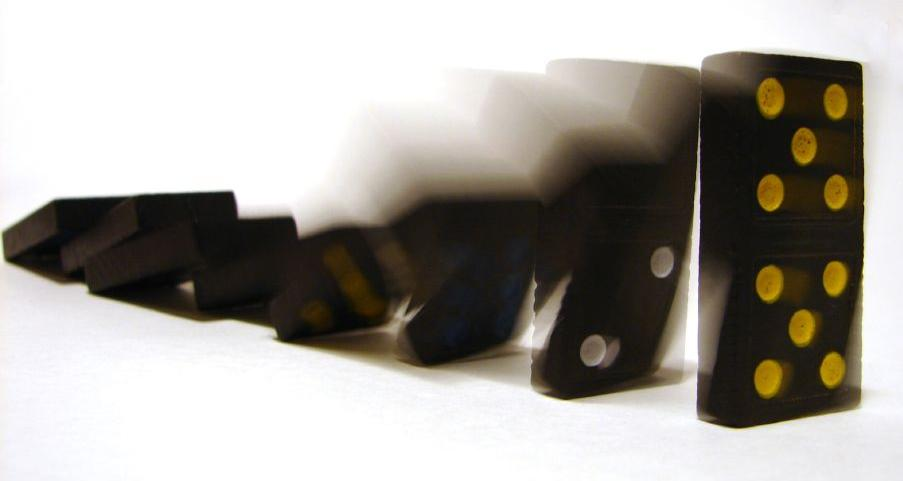
\includegraphics[width=2in]{../../resources/images/Domino_Cascade.jpeg}

    {\tiny Wikimedia commons\\ \href{https://creativecommons.org/licenses/by/2.0/legalcode}{https://creativecommons.org/licenses/by/2.0/legalcode} }
\end{center} 

\fbox{\parbox{\textwidth}{

{\bf Proof by Mathematical Induction}

To prove a universal quantification over the set of all integers greater than
or  equal to some  base integer $b$,

\vspace{-10pt}

\begin{itemize}
\item[] {\bf Basis Step}:  Show the property holds for $b$. 
\item[]  {\bf Recursive Step}:  Consider an arbitrary integer $n$ greater than or  equal to  $b$, assume
    (as the {\bf induction hypothesis})  that the property holds  for $n$, and use  this and
    other facts to  prove that  the property holds for $n+1$.
\end{itemize}

}} 

\fbox{\parbox{\textwidth}{

{\bf Proof by Strong Induction}

To prove that a universal quantification over the set of all integers greater than or equal to some  base integer $b$ holds,  pick a  fixed nonnegative integer  $j$ and then: \hfill 

\begin{tabularx}{\textwidth}{lX}
    {\bf Basis Step}: & Show the statement holds for $b$, $b+1$, \ldots, $b+j$. \\
    {\bf Recursive Step}: & Consider an arbitrary integer $n$ greater than or  equal to $b+j$, assume
    (as the {\bf strong  induction hypothesis})  that the property holds  for {\bf each of} $b$, $b+1$, \ldots, $n$, 	
    and use  this and
    other facts to  prove that  the property holds for $n+1$.
\end{tabularx}
}} 
 \newpage


{\bf Theorem}: Every positive integer is a sum of (one or more) distinct powers of $2$.
{\it Binary expansions exist!}

Recall the definition for binary expansion:



{\bf Definition} For $n$ a positive integer, 
the {\bf binary expansion of $n$}  is
\[
(a_{k-1} \cdots a_1 a_0)_b
\]
where $k$ is a positive integer, $a_0, a_1, \ldots, a_{k-1}$ 
are each $0$ or $1$, $a_{k-1} \neq  0$, and
\[
n =  \sum_{i=0}^{k-1} a_{i} b^{i}
\]
 

The idea in the ``Least significant first" algorithm 
for computing binary expansions is that the binary
expansion of {\it half} a number becomes {\it part} of the binary expansion of 
the number of itself. We can use this 
idea in a proof by strong induction that binary expansions exist for all 
positive integers $n$.


{\bf Proof by strong induction}, with $b=1$ and $j=0$.


{\bf Basis step}:  WTS property is true about  $1$.

\phantom{Choose $a_0 = 1$, then $(a_0)_2 = 1 \cdot 2^0 = 1$.}
\vspace{80pt}


{\bf Recursive step}: Consider an arbitrary integer $n \geq 1$.

Assume (as the strong induction hypothesis, IH) that the property is true about  each of $1, \ldots, n$.  

WTS that the property is true about $n+1$.

{\it Idea}: We will apply the IH to $(n+1) \textbf{ div } 2$.

{\it Why is this ok?}

\phantom{Notice that $(n+1) \textbf{ div } 2$ is greater than or equal to 
$1$ and less than or equal to $n$ because $n \geq 1$.}
\vspace{100pt}

{\it Why is this helpful?}

By the IH, we can write $(n+1) \textbf{ div } 2$ as 
a sum of powers of $2$. In other words, 
there are values $a_{k-1}, \ldots, a_0$ such that each $a_i$ is $0$ or $1$, $a_{k-1} = 1$, 
and
\[
    \sum_{i=0}^{k-1} a_i 2^i = (n+1) \textbf{ div } 2   
\]
Define the collection of coefficients
\[
   c_{j} = 
   \begin{cases}
        a_{j-1} \qquad&\text{if $1 \leq j \leq k$}\\
        (n+1) \textbf{ mod } 2 &\text{if $j = 0$}
   \end{cases}
\]
Calculating: 
\begin{alignat*}{2}
    \sum_{j=0}^k c_j 2^j &= c_0 + \sum_{j=1}^k c_j 2^j 
    = c_0 + \sum_{i=0}^{k-1} c_{i+1} 2^{i+1} &\qquad &\text{re-indexing the summation}\\
    &= c_0 + 2 \cdot \sum_{i=0}^{k-1} c_{i+1}2^i &\qquad &\text{factoring out a $2$ from each term in the sum}\\
    &= c_0 + 2 \cdot \sum_{i=0}^{k-1} a_{i} 2^i &\qquad &\text{by definition of $c_{i+1}$}\\
    &= c_0 + 2 \left(~(n+1) \textbf{ div } 2 ~\right) &\qquad &\text{by IH} \\
    &= \left(~ (n+1) \textbf{ mod } 2 ~\right ) + 2 \left(~(n+1) \textbf{ div } 2 ~\right) &\qquad &\text{by definition of $c_0$} \\
    &= n+1 &\qquad&\text{by definition of long division}
\end{alignat*}

Thus, $n+1$ can be expressed as a sum of powers of $2$, as required. 
\subsubsection*{Representing positive integers with primes}


{\bf Theorem}: Every positive integer {\it greater than 1} is a product of (one or more) primes.

{\bf Before we prove, let's try some examples}:

$20 = $

$100 = $

$5 = $


{\bf Proof by strong induction}, with $b=2$ and $j=0$.

{\bf Basis step}:  WTS property is true about  $2$.

Since $2$ is itself prime,
it is already written as a product of (one) prime.


{\bf Recursive step}: Consider an arbitrary integer $n \geq 2$.
Assume (as the strong induction hypothesis, IH) that the property is true about  each of $2, \ldots, n$.  
WTS that the property is true about  $n+1$: We want to show that $n+1$ can be written 
as a product of primes.  Notice that $n+1$ is itself prime or it is composite.

{\it Case 1}: assume $n+1$ is prime and then immediately it is written as a product
of (one) prime so we are done.  

{\it Case 2}: assume that $n+1$ is composite
so there are integers $x$ and $y$ where $n+1 = xy$ and each of them is between $2$ and $n$
(inclusive).  Therefore, the induction hypothesis applies to each of $x$ and $y$ so each 
of these factors of $n+1$ can be written as a product of primes.  Multiplying these products together, 
we get a product of primes that gives $n+1$, as required. 

Since both cases give the necessary
conclusion, the proof by cases for the recursive step is complete. \subsubsection*{Sending old-fashioned mail with postage stamps}


Suppose we had postage stamps worth $5$ cents and $3$ cents.
Which number of cents can we form using these stamps?
In other words, which postage can we pay?

$11$? 

$15$? 


$4$?



\begin{align*}
    &CanPay(0) \land \lnot CanPay(1) \land \lnot CanPay(2) \land \\
    &CanPay(3) \land \lnot CanPay(4) \land CanPay(5) \land CanPay(6) \\
    &\lnot CanPay(7) \land \forall n \in \mathbb{Z}^{\geq 8} CanPay(n)
\end{align*}

where the predicate $CanPay$ with domain $\mathbb{N}$ is
\[
    CanPay(n) = \exists x \in \mathbb{N} \exists y \in \mathbb{N}  ( 5x+3y = n)
\]


{\bf Proof} (idea): First, explicitly give witnesses or general arguments
for postages between $0$ and $7$. 
To prove the universal claim, we can use mathematical induction or strong induction.

{\it Approach 1, mathematical induction}: if we have
stamps that add up to $n$ cents, need to use them (and others)
to give $n+1$ cents. How do we get $1$ cent with just $3$-cent
and $5$-cent stamps?

\vspace{-10pt}
Either \underline{take away a $5$-cent stamps and add two $3$-cent stamps},

\vspace{-10pt}
or \underline{take away three $3$-cent stamps and add two $5$-cent stamps}.

\vspace{-10pt}
The details of this proof by mathematical induction
are making sure we have enough 
stamps to use one of these approaches.

{\it Approach 2, strong induction}: assuming we know how to make postage
for {\bf all} smaller values (greater than or equal to $8$), when
we need to make $n+1$ cents, \underline{add one $3$ cent stamp to 
however we make $(n+1) - 3$ cents}.

\vspace{-10pt}
The details of this proof by strong induction are making sure we 
stay in the domain of the universal when applying the induction hypothesis.
 \newpage
\subsection*{Review}
\begin{enumerate}
    \item \hspace{1in} \\ 

In class, we proved the theorem that: 
Every positive integer is a sum of (one or more) distinct powers of $2$.

What's wrong with the following {\it attempted} proof of this fact?


{\bf Attempted proof by mathematical induction}, with $b=1$.

{\bf Basis step}: WTS $1$ can be written 
as a sum of (one or more) distinct powers of $2$. Since $1 =2^0$, 
we are done.

{\bf Recursive step}: Consider an arbitrary integer $n \geq 1$.
By the IH, we can write $n$ as a sum of distinct powers of $2$.
Since $1 = 2^0$, it is a power of $2$ and we can add it as a term 
to this sum of powers of $2$. When we do so, the terms sum to $n+1$
and we are done.

\begin{enumerate}
\item The basis step is not sufficient.
\item The induction hypothesis is not stated correctly.
\item It's wrong to say that $1$ is a power of $2$.
\item Adding the $2^0$ to the sum of powers doesn't give the correct value.
\item Adding the $2^0$ to the sum of powers 
is problematic for a different reason.
\end{enumerate}
     \item \hspace{1in}\\ 


Recall that a prime factorization is a product of primes (potentially with some of the primes
occurring more than once).
Select all and only the correct prime factorizations of positive integers.

\begin{enumerate}
    \item $2\cdot 2 \cdot 2 \cdot 2$
    \item $3$
    \item $3 \cdot 4 \cdot 5$
    \item $17 \cdot 21$
    \item $2 \cdot 11$
\end{enumerate}     \newpage
    \item 

In this question, we'll consider two possible 
proofs of the statement
\[
    \forall n  \in  \mathbb{Z}^{\geq 8}  \exists x \in \mathbb{N}  \exists y \in \mathbb{N}  (  5x+3y =  n)
\]

\begin{enumerate}
\item First approach, using mathematical induction ($b=8$).

{\bf Basis step}:  WTS property is true about $8$.
Consider the witnesses $x = 1$, $y=1$. These 
are nonnegative integers and $5 \cdot 1 + 3 \cdot 1 = 8$, as
required.

{\bf Recursive step}: Consider an  arbitrary  $n \geq 8$.
Assume (as the induction hypothesis, IH) that there are nonnegative integers
$x, y$ such that $n =  5x +  3y$.  WTS
that there are nonnegative integers $x', y'$ such
that  $n+1 = 5x' +  3y'$.  We consider two cases, 
depending on  whether  any  $5$ cent stamps
are used for $n$.

{\it Case 1}:  Assume $x \geq  1$ (we assume that at least one
$5$ cent stamp is used for $n$).
Define $x' = x-1$ and $y'=y+2$ (both in  $\mathbb{N}$ by case assumption).


Calculating:
\begin{align*}
5x' +  3y' &\overset{\text{by def}}{=}  5(x-1) +  3(y+2)  = 5x -  5 +3y +   6  \\
&\overset{\text{rearranging}} = (5x+3y) -5  + 6\\
& \overset{\text{IH}}{=} n-5+6 =  n+1
\end{align*}


{\it  Case 2}: Assume $x = 0$.  Therefore  $n  = 3y$,  so 
since  $n \geq 8$, $y \geq 3$. Define $x' = 2$ and $y'=y-3$
(both in $\mathbb{N}$ by case assumption).
Calculating:
\begin{align*}
5x' +  3y' &\overset{\text{by def}}{=}  5(2) +  3(y-3)  = 10  +3y -9  \\
&\overset{\text{rearranging}} = 3y +10 -9 \\
&\overset{\text{IH and case}}{=} n+10-9 =  n+1
\end{align*}

Since the goal has been proved from each case, the proof by cases is complete and
we have proved the recursive step. $\square$\\


Why was the recursive step split into two cases?
\begin{enumerate}
    \item Because there are two variables $x$ and $y$ that need witnesses.
    \item Because the statement has alternating quantifiers $\forall$ and $\exists$
    \item Because the witness values need to be nonnegative and subtraction may lead to negative values.
    \item Because the domain is all integers greater than or equal to $8$.
    \item Because there are two steps in the recursive definition of $\mathbb{N}$
\end{enumerate}

\item  Second approach, by strong induction ($b=8$ and $j=2$)

{\bf Basis step}:  WTS property is true about  $8, 9, 10$
\begin{itemize}
\item Consider the witnesses $x = 1$, $y=1$. These 
are nonnegative integers and $5 \cdot 1 + 3 \cdot 1 = 8$, as
required.
\item Consider the witnesses $x = 0$, $y=3$. These 
are nonnegative integers and $5 \cdot 0 + 3 \cdot 3 = 9$, as
required.
\item Consider the witnesses $x = 2$, $y=0$. These 
are nonnegative integers and $5 \cdot 2 + 3 \cdot 0 = 10$, as
required.
\end{itemize}

{\bf Recursive step}: Consider an  arbitrary  $n \geq 10$.
Assume, as the strong induction hypothesis, 
that the property is true about each of $8, 9, 10, \ldots, n$.  
WTS
that there are nonnegative integers $x', y'$ such
that  $n+1 = 5x' +  3y'$. 

Since \underline{Blank 1}, 
by the strong induction hypothesis, there are nonnegative integers
$x, y$ such that $(n+1) - 3 = 5x + 3y$.
Choosing \underline{Blank 2} works because
\[
    5x' + 3y' = 5x + 3y + 3 = (n+1) - 3 + 3 = n+1.
\]

Choose a true and useful statement to fill in Blank 1.
    \begin{enumerate}
        \item $n \geq 10$ and hence $(n+1) - 3 \geq 8$
        \item $n \geq 8$ and hence $(n+1)-3 \geq 8$
        \item $n \geq 8$ and hence $(n+1) \geq 9$
    \end{enumerate}

Choose the appropriate statement to fill in Blank 2.
    \begin{enumerate}
        \item $x' = x, y' = y$
        \item $x' = x+1, y' = y+1$
        \item $x' = x+1, y' = y$
        \item $x' = x, y' = y+1$
        \item $x' = x-1, y' = y-1$
        \item $x' = x-1, y' = y$
        \item $x' = x, y' = y-1$
    \end{enumerate}
\end{enumerate}
 \end{enumerate}

\newpage
\section*{Wednesday November 10}

\subsubsection*{Finding a winning strategy for a game}


Consider the following game: two players start with 
two (equal) piles of jellybeans in front of them.
They take turns removing any positive integer number
of jellybeans at a time from one of two piles in 
front of them in turns.

The player who removes the last jellybean wins the game.

Which player (if any) has a strategy to guarantee
to win the game?


Try out some games, starting with $1$ jellybean in each pile,
then $2$ jellybeans in each pile, then $3$ jellybeans in each pile.
Who wins in each game?

\vspace{200pt}


Notice that reasoning about the strategy for the $1$ jellybean 
game is easier than about the strategy for the $2$ jellybean game.

{\it Formulate a winning strategy by working to 
transform the game to a simpler one we know we can win.}

\newpage

{\it Player 2's Strategy}: Take the same number of jellybeans that Player 1 did, 
but from the opposite pile. 


{\it Why is this a good idea}: If Player 2 plays this strategy, at the next turn
Player 1 faces a game with the same setup as the original, just with fewer
jellybeans in the two piles. Then Player 2 can keep playing this strategy to win.

{\bf Claim}: Player 2's strategy guarantees they will win the game.

{\bf Proof}: By strong induction, we will prove that for all positive 
integers $n$, Player 2's strategy guarantees a win in the game that starts with 
$n$ jellybeans in each pile.

{\bf Basis step}: WTS Player 2's strategy guarantees a win 
when each pile starts with $1$ jellybean.

In this case, Player 1 has to take the jellybean from one of the piles
(because they can't take from both piles at once).
Following the strategy, Player 2 takes the jellybean from the 
other pile, and wins because this is the last jellybean.

{\bf Recursive step}: Let $n$ be a positive integer. 
As the strong induction hypothesis, assume that
Player 2's strategy guarantees a win in the games 
where there are $1, 2, \ldots, n$ many jellybeans in each 
pile at the start of the game.

WTS that Player 2's strategy guarantees a win in the game where
there are $n+1$ in the jellybeans in each pile at the start of the game.

In this game, the first move has Player 1 take 
some number, call it $c$ (where $1 \leq c \leq n+1$),
of jellybeans from one of the piles. 
Playing according to their strategy, Player 2 then 
takes the same number of jellybeans from  the other pile.

Notice that $(c = n+1) \lor (c \leq n)$.

{\it Case 1}: Assume $c = n+1$, then in their first move, 
Player 2 wins because they take all of the second pile, which 
includes the last jellybean.

{\it Case 2}: Assume $c \leq n$. Then after Player 2's first move,
the two piles have an equal number of jellybeans. The number
of jellybeans in each pile is 
\[
    (n+1) - c
\]
and, since $1 \leq c \leq n$, this number is between $1$ and $n$.
Thus, at this stage of the game, the game appears identical to a new 
game where the two piles have an equal number of jellybeans between $1$
and $n$. Thus, the strong induction hypothesis applies, and Player 2's
strategy guarantees they win.

 \newpage


\fbox{\parbox{\textwidth}{

{\bf New! Proof by Contradiction} 

To prove that a statement $p$ is true, pick another statement $r$ and once we show
that $\neg p  \to (r \wedge  \neg r)$ then  we can conclude that  $p$ is  true.

{\it Informally} The statement we care about can't possibly be false, so it must be true.
}} 

 \subsection*{Least and greatest}


For a set of numbers $X$, how do you formalize ``there is a greatest $X$'' 
or ``there is a least $X$''?

\vspace{30pt}

{\bf Prove} or {\bf  disprove}:  There is a least prime number.

\vspace{100pt}

{\bf Prove} or {\bf  disprove}: There is a greatest integer. 

{\it Approach 1, De Morgan's and universal generalization}: 

\vspace{100pt}

{\it Approach 2, proof by contradiction}: 

\vspace{200pt}

{\it Extra examples}: 
Prove or disprove that $\mathbb{N}$,  $\mathbb{Q}$ each have a
least and a greatest element. 
 
\newpage
\subsection*{Review}
\begin{enumerate}
\item \hspace{1in}\\ 

Recall the game Nim from class.

\begin{enumerate}
    \item Why did we use strong induction to prove that Player 2's strategy guarantees a win?
    \begin{enumerate}
        \item Because there are two players in the game.
        \item Because each turn can involve a player taking some positive number 
        of jellybeans from a pile, not just one jellybean.
        \item Because the strategy player 2 uses depends on what player 1 does.
        \item Because the set of natural numbers is recursively defined.
    \end{enumerate}
    \item  If we modify the game so that in each turn, a player could take jellybeans
    from one or both piles, which player has a winning strategy?
    \begin{enumerate}
        \item Player 1.
        \item Player 2.
        \item Neither in general, the existence of a winning strategy for the players depends 
        on how many jellybeans are in each pile to start.
    \end{enumerate}
    \item  If we modify the game so that in each turn, a player must take 
    exactly one jellybean, which player has a winning strategy?
    \begin{enumerate}
        \item Player 1.
        \item Player 2.
        \item Neither in general, the existence of a winning strategy for the players depends 
        on how many jellybeans are in each pile to start.
    \end{enumerate}
\end{enumerate}
 \item \hspace{1in}\\ 

We will prove that there is no greatest prime number

{\bf Proof} Assume, towards a \underline{BLANK1}, that 
there is a greatest prime number, call it $n_{BIG}$.
In particular, this means that there are finitely many 
primes. Let's label them in order $p_1, \ldots, p_n$ where 
$p_1 = 2$ and $p_n = n_{BIG}$.
Choose $r = $ \underline{BLANK2}. We proved in class
that $r$ is {\bf true}. It remains to show that (under our 
assumption) $r$ is {\bf false}, because
that would complete the contradiction argument.
Define the integer
\[
    C = (p_1 \cdots p_n) + 1
\]
This is a positive integer greater than $1$. 
However, we will show that it does not have any prime
factors and thus is not a product of primes.
By our assumption, the only prime numbers are $p_1, \ldots, 
p_n$. Thus, to show that $C$ does not have any prime
factors means to show that $p_i$ is not a factor 
of $C$ for each value of $i$ from $1$ to $n$. 
Towards a universal generalization, let $i$ be an arbitrary
between $1$ and $n$ (inclusive). We need to prove that $p_i$ is 
not a factor of $C$. By definition of $C$,
\[
    C = p_i ( p_1 \cdots p_{i-1} p_{i+1} \cdots p_n) + 1
\]
so $C \textbf{ div } p_i = p_1 \cdots p_{i-1} p_{i+1} \cdots p_n$
and $C \textbf{ mod } p_i = 1$ (because $p_i > 1$ since it is prime).
Since $C \textbf{ mod } p_i \neq 0$, $p_i$ is not a factor of $C$.
Thus $C$ witnesses that the universal claim is false, 
and we have proved that $r$ is false.




\begin{enumerate}
\item BLANK1
    \begin{enumerate}
        \item universal generalization
        \item proof of existential by witness
        \item direct proof
        \item proof by contrapositive
        \item proof by cases
        \item proof by contradiction
    \end{enumerate}
\item BLANK2
\begin{enumerate}
    \item The least prime number is $2$.
    \item There is a greatest prime number.
    \item There is a least prime number.
    \item Every positive integer greater than $1$ is a product of primes.
    \item Every positive integer has a base expansion.
    \item There is a greatest integer.
    \item There is no greatest integer.
\end{enumerate}
\end{enumerate} \item \hspace{1in}\\ 

Select all and only the situations in which the given
proof strategy would be available.

\begin{enumerate}
\item When might it be appropriate to use induction?
    \begin{enumerate}
        \item To prove that an existential claim over the set of integers is true.
        \item To prove that a universal claim over the real numbers is true.
        \item To prove that a conditional claim is true.
        \item None of the above.
    \end{enumerate}
\item When might it be appropriate to use proof by contradiction?
    \begin{enumerate}
        \item To prove that an existential claim over the set of integers is true.
        \item To prove that a universal claim over the real numbers is true.
        \item To prove that a conditional claim is true.
        \item None of the above.
    \end{enumerate}
\end{enumerate}
 \end{enumerate}

\newpage
\section*{Friday November 12}



{\bf Definition}: {\bf Greatest common divisor} Let $a$ and $b$ be integers, not both zero. The largest integer $d$ such that 
$d$ is a  factor of $a$ and $d$ is a factor of  $b$ is called the greatest common divisor of $a$ and $b$ 
and is denoted by $gcd(~(a, b)~)$. 

Why do we restrict to the situation where $a$ and $b$ are not both zero?

\vspace{50pt}


Calculate $gcd(~(10,15)~)$

\vspace{50pt}

Calculate $gcd(~(10,20)~)$

\vspace{50pt} 

{\bf Claim}: For any integers $a,b$ (not both zero), $gcd(~(a,b)~) \geq 1$.

{\bf Proof}: {\it Show that $1$ is a common factor of any two integers, so since the gcd 
is the greatest common factor it is greater than or equal to any common factor.}

\vspace{150pt}

{\bf Claim}: For any positive integers $a,b$, $gcd(~(a,b)~) \leq a$ and $gcd( ~(a,b)~) \leq b$.

{\bf Proof} {\it Using the definition of gcd and the fact that factors of a positive integer
are less than or equal to that integer.}

\vspace{150pt}

{\bf Claim}: For any positive integers $a,b$, if $a$ divides $b$ then $gcd(~(a,b)~) = a$.

{\bf Proof} {\it Using previous claim and definition of gcd.}

\vspace{150pt}


{\bf Claim}: For any positive integers $a,b,c$, if there is some integer $q$ such that $a = bq + c$,
\[
    gcd(~(a,b)~) = gcd (~(b,c)~)
\]
{\bf Proof} {\it Prove that any common divisor of $a,b$ divides $c$ and that any common 
divisor of $b,c$ divides $a$.}

\vspace{150pt}
 

{\bf Lemma}: For any integers $p, q$ (not both zero), 
$gcd \left(~ \left(~\frac{p}{gcd(~(p,q)~)}, \frac{q}{gcd(~(p,q)~)} ~\right) ~\right) = 1$ .
In other words, can reduce to relatively prime integers by dividing by gcd.

{\bf Proof}:

Let $x$ be arbitrary positive integer and assume that $x$ is a 
factor of each of $\frac{p}{gcd(~(p,q)~)}$ and $\frac{q}{gcd(~(p,q)~)}$. 
This gives integers $\alpha$, $\beta$ such that 
\[
    \alpha x = \frac{p}{gcd(~(p,q)~)} \qquad \qquad \beta x = \frac{q}{gcd(~(p,q)~)}
\]
Multiplying both sides by the denominator in the RHS: 
\[
    \alpha x \cdot gcd(~(p,q)~)= p \qquad \qquad \beta x \cdot gcd(~(p,q)~)= q
\]
In other words, $x \cdot gcd(~(p,q)~)$ is a common divisor of $p, q$. By definition of $gcd$, this means
\[
    x \cdot gcd (~(p,q)~) \leq gcd (~(p,q)~)
\]
and since $gcd(~(p,q)~)$ is positive, this means, $x \leq 1$.
\vspace{350pt}
 
\newpage
\subsection*{Sets of numbers}

We've seen multiple representations of the set of positive integers
(using base expansions and using prime factorization). Now we're 
going to expand our attention to other sets of numbers as well.


The {\bf set  of rational numbers}, $\mathbb{Q}$  is defined as 
\[
\left\{ \frac{p}{q} \mid p \in \mathbb{Z}  \text{ and  } q  \in \mathbb{Z} \text{ and } q \neq  0 \right\}
\text{~~~~or, equivalently,~~~~}
\{ x  \in  \mathbb{R} \mid \exists p \in \mathbb{Z}  \exists q \in \mathbb{Z}^+ ( p =  x \cdot q) \}
\]

{\it Extra practice}: Use the definition of set equality to prove that the definitions above  give the same set.

 

We have the following subset relationships between sets of numbers:

\[
    \mathbb{Z}^{+} \subsetneq \mathbb{N} \subsetneq \mathbb{Z} \subsetneq \mathbb{Q} \subsetneq \mathbb{R}
\]


Which of the proper subset inclusions above can you prove?

\vspace{50pt} 

{\bf Goal}:  The square root of $2$ is not a rational number.  In other words: $\neg \exists x \in \mathbb{Q} ( x^2 -  2 = 0)$

{\bf Attempted proof}: The definition of the set of rational numbers is the collection of fractions $p/q$ where $p$ is an integer and $q$ is a nonzero integer. Looking for a {\bf witness} $p$ and $q$, we can write the square root of $2$ as the fraction 
$\sqrt{2 }/1$, where $1$ is a nonzero integer. Since the numerator is not in the domain, this witness is not allowed, and we have shown that the square root of $2$ is not a fraction of integers (with nonzero denominator). Thus, the square root of $2$ is not rational.


{\it The problem in the above attempted proof is that} \underline{\phantom{it only considers one candidate witness
and does not prove that no witnesses exist.}}


{\bf Lemma 1:} For every two integers $a$ and  $b$, not both zero, with  $gcd(~(a,b)~) = 1$, it is not the case that both $a$
is  even and $b$ is even.


{\bf Lemma 2:} For every integer  $x$, $x$ is  even if and only if $x^2$  is even.


{\bf Proof}: Towards a proof by contradiction, we will define a statement 
$r$ such that $\sqrt{2} \in \mathbb{Q} \to (r \land \lnot r)$. 

Assume that $\sqrt{2} \in \mathbb{Q}$. Namely, there are positive integers
$p, q$ such that 
\[
    \sqrt{2} = \frac{p}{q}
\]
Let $a= \frac{p}{gcd( ~(p,q)~)}$, $b = \frac{q}{gcd(~(p,q)~)}$, then 
\[
    \sqrt{2} = \frac{a}{b} \qquad \text{and} \qquad gcd(~(a,b)~) = 1
\]

By Lemma 1, $a$ and $b$ are not both even. We define $r$ to be the 
statement ``$a$ is even and $b$ is even'', and we have proved $\lnot r$.

Squaring both sides and clearing denominator: $2b^2 = a^2$.

By definition of even, since $b^2$ is an integer$, a^2$ is even.

By Lemma 2, this guarantees that $a$ is even too. So, by 
definition of even, there is some integer (call it $c$), such that $a = 2c$.

Plugging into the equation:
\[
    2b^2 = a^2 = (2c)^2 = 4c^2
\]
and dividing both sides by $2$
\[
    b^2 = 2c^2
\]
and since $c^2$ is an integer, $b^2$ is even. By Lemma 2, $b$ is even too.
Thus, $a$ is even and $b$ is even and we have proved $r$. 

In other words, assuming that $\sqrt{2} \in \mathbb{Q}$ guarantees $r \land \lnot r$, 
which is impossible, so $\sqrt{2} \notin \mathbb{Q}$. QED

 
\newpage
\subsection*{Review}
\begin{enumerate}
\item \hspace{1in}\\ 

We will consider two ways for calculating the gcd. In each 
part of the question, you'll calculate $gcd(~(306, 120)~$).

\begin{enumerate}
\item The first approach uses some of the claims we proved in class
to get the following algorithm:


\begin{algorithm}[caption={Euclidean algorithm for calculating greatest common divisor}]
    procedure $\textit{Euclidean}$($a$: a positive integer, $b$: a positive integer)
    $x$ := $a$
    $y$ := $b$
    while $y \neq 0$
      $r$ := $x \textbf{ mod } y$
      $x$ := $y$
      $y$ := $r$
    return $x$ $\{ \textrm{the result of } gcd(~(a,b)~)\} $
\end{algorithm} 
Tracing this algorithm, lines 2 and 3 initialize the variables 
\[
    x:= 306 \qquad y:=120
\]
Entering the while loop, the variable $r$ is initialized to
\[
    r:= 66
\]
because $306 = 2 \cdot 120 + 66$ so $306 \textbf{ mod } 120 = 66$.
Calculate and fill in the updated value of $r$ in each subsequent iteration
of the {\bf while} loop, and then give the value of $gcd(~(306, 120)~$).

\item The second approach uses the representation of positive integers
greater than $1$ as products of primes. To calculate $gcd(~(a,b)~)$ we 
find the prime factorizations of each of $a$ and $b$, and then calculate
the number that results from multiplying together terms $p^c$ where $p$ is 
a prime that appears in {\it both} prime factorizations of $a$ and $b$
and $c$ is the {\it minimum} number of times $p$ appears in the two factorizations.

Select the prime factorizations for $306$ and $120$ and express their 
$gcd$ as a product of powers of primes.

Possible factorizations:
\begin{enumerate}
        \item $306 = 2 \cdot 153$, $120 = 2 \cdot 60$
        \item $306 = 1 \cdot 2 \cdot 3 \cdot 3 \cdot 17$, $120 = 1 \cdot 3 \cdot 5 \cdot 8$
        \item $306 = 2 \cdot 3 \cdot 3 \cdot 17$, $120 = 2 \cdot 2 \cdot 2 \cdot 3 \cdot 5$
\end{enumerate}

Possible $gcd$ choices:
\begin{enumerate}
\item $2$
\item $2 \cdot 3$
\item $5 \cdot 17$
\item $2^3 \cdot 3^2$
\item $2^3 \cdot 3^2 \cdot 5 \cdot 8 \cdot 17$
\end{enumerate}
\end{enumerate} \newpage
\item \hspace{1in}\\ 

{\it Goals for this question: recognize that we can prove the same statement
in different ways.  Trace proofs and justify why they are valid.}

Below are two proofs of the same statement: fill in the blanks with the 
expressions below.

{\bf Claimed statement}:  \textbf{(a)}$\underline{\phantom{\hspace{1.3in}}}$
\begin{quote}

{\bf Proof 1}: Using De Morgan's law for quantifiers, 
we can rewrite this statement as a universal of the negation of the body of the statement.
Towards a proof by universal generalization, let $x$ be an arbitrary element of $\mathbb{Z}$. Then we need to show that
$$\textbf{(b)}\underline{\phantom{\hspace{1.3in}}}$$

We proceed by contradiction to show that $$(x \textrm{ is odd} \land x^2 \textrm{ is even}) \to \textbf{(c)}\underline{\phantom{\hspace{1.3in}}}$$
We assume by direct proof that $(x \textrm{ is odd} \land x^2 \textrm{ is even})$. Then, $(x^2 \textrm{ is even})$ follows directly from this assumption, so by definition 
of conjunction, we must show that $(x^2 \textrm{ is not even})$ to complete the proof.
From the assumption, we have that $(x \textrm{ is odd})$.  Applying the definition of odd, $x = 2k + 1$ for some $k \in \mathbb{Z}$. Then $x^2 = 4k^2 + 4k + 1$. We can rewrite the right hand side to $2(2k^2 + 2k) + 1$. This shows that $x^2$ is odd by the definition of odd, since choosing $j = 2k^2 + 2k$ gives us $j \in \mathbb{Z}$ with $x^2 = 2j + 1$. Since a number is either even or odd and not both, and $x^2$ is odd, then it must not be even. 
This concludes the proof, as we have assumed the negation of the original statement and deduced a contradiction
from this assumption.
\end{quote}

\newpage
\begin{quote}{\bf Proof 2}: 

    \begin{tabular}{l p{2.5in}}
    1. \begin{tabular}{l}
        \textbf{To Show} $\forall x \in \mathbb{Z} \neg (x \textrm{ is odd} \land x^2 \textrm{ is even})$\\
    \end{tabular}
    & Rewriting statement using De Morgan's law for quantifiers
 \\ 
   2. \begin{tabular}{l}
        \textbf{Choose arbitrary} $x \in\mathbb{Z}$ \\
        \textbf{To Show} \textbf{(d)}$\underline{\phantom{\hspace{1.3in}}}$\\
    \end{tabular}
    & By \textbf{(e)}$\underline{\phantom{\hspace{1.3in}}}$\\
 \\
    3. \begin{tabular}{l}
        \textbf{To Show}
         $x \textrm{ is odd} \to \neg  (x^2 \textrm{ is even})$
    \end{tabular}
    & Rewrite previous {\bf To Show} using logical equivalence
    \\
    4. \begin{tabular}{l}
        \textbf{Assume } $x \textrm{ is odd}$ \\
        \textbf{To Show } $\neg  (x^2 \textrm{ is even})$ \\
    \end{tabular}
    & By \textbf{(f)}$\underline{\phantom{\hspace{1.3in}}}$\\
    \\    
    5. \begin{tabular}{l}
        \textbf{To Show} $x^2 \textrm{ is odd}$
    \end{tabular}
    & Rewrite previous {\bf To Show} using definition of even, odd
    \\
    6. \begin{tabular}{l}
        \textbf{Use the witness} $k$, an integer,\\
        where $x = 2k+1$\\
    \end{tabular}
     & By existential definition of $x$ being odd \\
    \\
    7. \begin{tabular}{l}
        \textbf{Choose the witness} \\
        $j = 2k^2 + 2k$, an integer\\
        \textbf{To Show} $x^2 = 2j+1$
    \end{tabular}
     & Show this new {\bf To Show} is true to prove the existential definition of $x^2$ being odd\\
    \\
    8.\begin{tabular}{l}
        \textbf{To Show} $(2k+1)^2  = 2j+1$
    \end{tabular}
    & Rewrite previous {\bf To Show} using definition of $k$
    \\
    9.  \begin{tabular}{l}
        \textbf{To Show} $(2k+1)^2  = 2(2k^2 + 2k) + 1$
    \end{tabular}
    & Rewrite previous {\bf To Show} using definition of $j$
    \\
    10. \begin{tabular}{l}
        \textbf{To Show } $T$ \\
    \end{tabular}
     & By algebra: multiplying out the LHS; factoring the RHS\\
    QED & Because we got to $T$ only by rewriting \textbf{To Show} to equivalent statements, using valid proof techniques and definitions. \\
    \end{tabular}
\end{quote}


Consider the following expressions as options to fill in the two proofs above. Give your answer as one of the numbers below for each blank a-c. You may use some numbers for more than one blank, but each letter only uses one of the expressions below.

\begin{multicols}{2}
\begin{enumerate}[label=\roman*.]
    \item $\exists x \in \mathbb{Z} \, (x \textrm{ is odd} \land x^2 \textrm{ is even})$
    \item $\neg \exists x \in \mathbb{Z} \, (x \textrm{ is odd} \land x^2 \textrm{ is even})$
    \item $\exists x \in \mathbb{Z} \, (x \textrm{ is odd} \land x \textrm{ is even})$
    \item $\neg \exists x \in \mathbb{Z} \, (x \textrm{ is odd} \land x \textrm{ is even})$
    \item $\exists x \in \mathbb{Z} \, (x^2 \textrm{ is odd} \land x^2 \textrm{ is even})$
    \item $\neg \exists x \in \mathbb{Z} \, (x^2 \textrm{ is odd} \land x^2 \textrm{ is even})$
    \item $(x^2 \textrm{ is even} \land x^2 \textrm{ is not even})$
    \item $\neg (x \textrm{ is odd} \land  x^2 \textrm{ is even})$
    \item $(x \textrm{ is odd} \land  x^2 \textrm{ is even})$
    \item $(x \textrm{ is odd} \land  x \textrm{ is not odd})$
    \item $\neg (x \textrm{ is odd} \land  x \textrm{ is not odd})$
    \item $x^2 \textrm{ is even}$
    \item $x^2 \textrm{ is odd}$
    \item universal generalization
    \item proof by cases
    \item direct proof
    \item proof by contraposition
    \item proof by contradiction
\end{enumerate}
\end{multicols}
 \end{enumerate}

\newpage 


\section*{Monday November 15}



We have the following subset relationships between sets of numbers:

\[
    \mathbb{Z}^{+} \subsetneq \mathbb{N} \subsetneq \mathbb{Z} \subsetneq \mathbb{Q} \subsetneq \mathbb{R}
\]


Which of the proper subset inclusions above can you prove?

\vspace{50pt} 

{\bf Definition}: A {\bf finite} set is one whose distinct elements can be counted by a natural number.
 

{\bf Motivating question}: when can we say one set is {\it bigger than} another?

Which is bigger? 
\begin{itemize}
    \item The set $\{1,2,3\}$ or the set $\{0,1,2,3\}$?
    \item The set $\{0, \pi, \sqrt{2} \}$ or the set $\{\mathbb{N}, \mathbb{R}, \emptyset\}$?
    \item The set $\mathbb{N}$ or the set $\mathbb{R}^+$?
\end{itemize}

{\it Which of the sets above are finite? infinite?} 

{\bf Key idea for cardinality}: Counting 
distinct elements is a way of labelling elements
with natural numbers. This is a function!
In general, functions let us 
associate elements of one set with those
of another. If the association is ``{\it good}", 
we get a correspondence between the elements of the subsets
which can relate the sizes of the sets. 

{\it Analogy}: Musical chairs

\begin{multicols}{2}
\includegraphics[width=1.8in]{../../resources/images/musicalchairs.png}
\columnbreak

People try to sit down when the music stops

Person\sun~ sits in Chair 1,
Person\smiley~ sits in Chair 2,

Person\frownie~  is left standing!
\end{multicols}
What does this say about the number of chairs and the number of people?

\vspace{100pt} \newpage


Recall that a function is defined by its (1) domain, (2) codomain, and (3) rule assigning each 
element in the domain exactly one element in the codomain. 
The domain and codomain are nonempty sets.
The rule can be depicted as a table, formula, English description, etc.

A function can {\it fail to be well-defined} if there is some 
domain element where the function rule doesn't give a
unique codomain element. For example, the function rule might lead to 
more than one potential image, or to an image outside of the codomain.


{\it Example}: $f_A: \mathbb{R}^+ \to \mathbb{Q}$ with $f_A(x) = x$ is {\bf not} a well-defined function because

\vspace{100pt}


{\it Example}: $f_B: \mathbb{Q} \to \mathbb{Z}$ with $f_B\left(\frac{p}{q}\right) = p+q$ is {\bf not} a well-defined function because

\vspace{100pt}


{\it Example}: $f_C: \mathbb{Z} \to \mathbb{R}$ with $f_C(x) = \frac{x}{|x|}$ is {\bf not} a well-defined function because

\vspace{100pt}
 

{\bf Definition} : A function $f: D  \to C$ is {\bf one-to-one} (or  injective) 
means for every $a,b$ in the domain $D$, 
if $f(a) = f(b)$ then  $a=b$.

Formally, $f: D  \to  C$ is  one-to-one  means $\underline{\phantom{\forall a \in D \forall b \in D ~(f(a) = f(b) \to a = b)}}$.
 

Informally, a function being one-to-one means ``no duplicate images''.

\phantom{Draw finite domain, finite codomain picture with duplicate image.}
\vspace{50pt} 

{\bf Definition}:  For nonempty sets $A, B$, we say that {\bf the  cardinality of $A$ is  no  bigger than the cardinality of $B$}, 
and write $|A| \leq |B|$, to mean there is a  one-to-one function  with domain $A$  and codomain $B$.
Also, we define $|\emptyset| \leq |B|$ for all sets $B$. 

{\it In the analogy}: The function $sitter: \{ Chair1, Chair2\} \to \{ Person\sun, Person\smiley, Person\frownie \}$ given
by $sitter(Chair1) = Person\sun$,  $sitter(Chair2) = Person\smiley$, is one-to-one and witnesses that 
\[
| \{ Chair1, Chair2\} | \leq |\{ Person\sun, Person\smiley, Person\frownie \}|
\] 

Let $S_2$ be the set of RNA strands of length 2, formally $S_2 = \{ s \in S \mid rnalen(s) = 2\}$.

{\bf True} or {\bf False}: $| \{\A,\U,\G,\C\} | \leq |S_2 |$ 

{\it Why?}
\vspace{80pt}

{\bf True} or {\bf False}: $| \{\A,\U,\G,\C\} \times \{\A, \U, \G,\C\} | \leq |S_2 |$

{\it Why?}
\vspace{80pt}
 

{\bf Definition}: A function $f: D  \to C$ is {\bf onto} (or  surjective) means for every $b$ in the codomain, 
there  is an element $a$ in the domain with  $f(a) = b$.

Formally, $f: D  \to  C$ is  onto  means $\underline{\phantom{\forall b \in C  \exists a \in D ( f(a) = b)}}$.
 

Informally, a function being onto means ``every potential image is an actual image''.

\phantom{Draw finite domain, finite codomain picture with duplicate image.}
\vspace{50pt} 

{\bf Definition}:  For nonempty sets $A, B$, we say that {\bf the  cardinality of $A$ is  no  smaller than 
the cardinality of  $B$}, and 
write $|A| \geq |B|$, to mean there is an onto function  with domain $A$  and codomain $B$.
Also, we define $|A| \geq |\emptyset|$ for all sets $A$.
 

{\it In the analogy}: The function $triedToSit: \{ Person\sun, Person\smiley, Person\frownie \} \to  \{ Chair1, Chair2\} $ given
by $triedToSit(Person\sun) = Chair1$,  $triedToSit(Person\smiley) = Chair2$, 
$triedToSit(Person\frownie) = Chair2$, is onto and witnesses that 
\[
 |\{ Person\sun, Person\smiley, Person\frownie \}| \geq | \{ Chair1, Chair2\} |
\] \newpage


Let $S_2$ be the set of RNA strands of length 2.

{\bf True} or {\bf False}: $ |S_2 | \geq | \{\A,\U,\G,\C\} |$

{\it Why?}
\vspace{80pt}

{\bf True} or {\bf False}: $ |S_2 | \geq | \{\A,\U,\G,\C\} \times \{\A, \U, \G,\C\} |$

{\it Why?}
\vspace{80pt} 

{\bf Definition} : A function $f: D  \to C$ is a {\bf bijection} means that it is both 
one-to-one  and onto. The {\bf inverse} of a  bijection $f: D  \to  C$ is 
the function $g: C  \to  D$  such that $g(b) = a$ iff  $f(a) =  b$.
 \subsection*{Cardinality of sets}

For nonempty sets $A, B$ we say
\begin{align*}
|A| \leq |B| &\text{ means there is a one-to-one function with domain $A$, codomain $B$} \\
|A| \geq |B| &\text{ means there is an onto function with domain $A$, codomain $B$} \\
|A| = |B| &\text{ means there is a bijection with domain $A$, codomain $B$}
\end{align*}

For all sets $A$, we say $|A| = |\emptyset|$, $|\emptyset| = |A|$ if and only if $A = \emptyset$. 

{\it Caution}: we use 
familiar symbols to define cardinality, like
$| \phantom{\cdots} | \leq | \phantom{\cdots} |$
and 
$| \phantom{\cdots} | \geq | \phantom{\cdots} |$
and 
$| \phantom{\cdots} | = | \phantom{\cdots} |$, 
but the meaning of these symbols depends on context.
We've seen that vertical lines can mean absolute
value (for real numbers), divisibility (for integers), 
and now sizes (for sets). 

Now we see that $\leq$ and $\geq$ can mean comparing
numbers or comparing sizes of sets. When the sets being 
compared are finite, the definitions 
of $|A| \leq |B|$ agree. 

But, properties of numbers cannot be assumed when comparing
cardinalities of infinite sets.

In a nutshell: cardinality of sets is defined via functions.
This definition agrees with the usual notion of ``size'' for 
finite sets. \newpage
\section*{Review}
\begin{enumerate}
    \item \hspace{1in}\\ 

Select all and only the {\bf finite} sets below.

\begin{enumerate}
\item $X = \{ a,b,c\}$
\item $Y = \{ 1, 2, 3, 4, 5\}$
\item $Z = \{ 10, 20, 30 \}$
\item $\emptyset$
\item $\mathbb{Z}$
\item $\{ \emptyset \}$
\item $\{ \mathbb{Z} \}$
\end{enumerate}     \item \hspace{1in}\\ Consider the following input-output definition tables with $X = \{ a,b,c\}$ and 
$Y = \{ 1, 2, 3, 4, 5\}$ and $Z = \{ 10, 20, 30 \}$

\begin{center}
\begin{multicols}{3}
\begin{tabular}{c}
Table 1\\
 \begin{tabular}{c|c}
Input & Output \\
\hline
$1$ & $10$ \\
$2$ & $20$ \\
$3$ & $30$ \\
\end{tabular}\end{tabular}
\columnbreak
\begin{tabular}{c}
Table 2\\ 
\begin{tabular}{c|c}
Input & Output \\
\hline
$a$ & $1$ \\
$b$ & $4$ \\
$c$ & $5$ \\
\end{tabular}\end{tabular}
\columnbreak
\begin{tabular}{c}
Table 3\\ 
\begin{tabular}{c|c}
Input & Output \\
\hline
$10$ & $a$ \\
$20$ & $b$ \\
$30$ & $a$ \\
\end{tabular}\end{tabular}
\end{multicols}
\end{center}

\begin{enumerate}
\item Select all and only the tables that each define a well-defined function 
whose domain and codomain 
is each $X$, $Y$, or $Z$.
\item Select all and only the tables that each define a well-defined function 
(with domain $X$ or $Y$ or $Z$ and 
with codomain $X$ or $Y$ or $Z$) and that is one-to-one.
\item Select all and only the tables that each define a well-defined function 
(with domain $X$ or $Y$ or $Z$ and 
with codomain $X$ or $Y$ or $Z$) and that is onto.
\end{enumerate}     \newpage
    \item \hspace{1in}\\ 

Consider the following functions:

\[
\begin{array}{l|l}
\begin{array}{ll}
f : \mathbb{Z} &\to \mathbb{N} \\
f(n) & = \begin{cases}
  0 & \textrm{ when } n = 0 \\
  (-2 \cdot n) - 1 & \textrm{ when } n < 0 \\
  2 \cdot n & \textrm{ when } n > 0
\end{cases}
\end{array}
&
\begin{array}{ll}
g : \mathbb{Z} &\to \mathbb{N} \\
g(n) & = \begin{cases}
  -1 \cdot n & \textrm{ when } n < 0 \\
  n & \textrm{ when } n \geq 0
\end{cases}
\end{array} \\
\hline

\begin{array}{ll}
h : \mathbb{N} &\to \mathbb{Z} \\
h(n) & = \begin{cases}
  (-2 \cdot n) + 1 & \textrm{ when } n \textrm{ is even } \\
  2 \cdot n & \textrm{ when } n \textrm{ is odd }
\end{cases}
\end{array}
&
\begin{array}{ll}
q : \mathbb{N} &\to \mathbb{Z} \\
q(n) & = \begin{cases}
  -1 \cdot ((n + 1) \textbf{ div } 2) & \textrm{ when } n \textrm{ is odd} \\
  n \textbf{ div } 2 & \textrm{ when } n \textrm{ is even} \\
\end{cases}
\end{array} \\
\end{array}
\]

\begin{enumerate}
\item What is the result of $f(-3)$?

\item What is the result of $q(f(-4))$?

 {\it Notice we are looking at function composition here: first apply $f$ and then apply 
 $q$ to the result.}

\item What is the result of $f(h(4))$? 

{\it Notice we are looking at function composition here: first apply $h$ and then apply 
$f$ to the result.}

\item What is the result of $g(-4)$?

\item What is the result of $g(4)$?

\item Consider the following statements, and indicate if they are true for each of $f$, $g$, $h$, and $q$.

\begin{enumerate}[label=\roman*.]
    \item This function is one-to-one.
    \item This function is onto.
    \item This function is a bijection.
    \item This function could serve as a witness for $|\mathbb{Z}| \leq |\mathbb{N}|$.
    \item This function could serve as a witness for $|\mathbb{Z}| \geq |\mathbb{N}|$.
    \item This function could serve as a witness for $|\mathbb{N}| \leq |\mathbb{Z}|$.
    \item This function could serve as a witness for $|\mathbb{N}| \geq |\mathbb{Z}|$.
\end{enumerate}

\end{enumerate} \end{enumerate}
\newpage

\section*{Wednesday November 17}


{\bf Properties of cardinality}
\begin{align*}
&\forall A ~ (~  |A| = |A| ~)\\
&\forall A ~ \forall B ~(~ |A| = |B|  ~\to ~ |B| = |A|~)\\
&\forall A ~ \forall B ~ \forall C~ (~ (|A| = |B| ~\wedge~ |B| = |C|) ~\to ~ |A| = |C|~)
\end{align*}

{\it Extra practice with proofs:} Use the definitions of bijections to prove these properties. \vspace{100pt}


{\bf Cantor-Schroder-Bernstein Theorem}: For all nonempty sets,
\[
|A| = |B| \qquad\text{if and only if} \qquad (|A| \leq |B| ~\text{and}~ |B| \leq |A|)
\qquad\text{if and only if} \qquad (|A| \geq |B| ~\text{and}~ |B| \geq |A|)
\]

To prove $|A| = |B|$,  we can do any {\bf one} of the following

\begin{itemize}\setlength{\itemsep}{-5pt}
\item Prove there exists  a bijection $f:  A \to B$;
\item Prove there exists a  bijection  $f: B  \to  A$;
\item Prove there exists two functions $f_1: A \to B$, $f_2: B \to  A$ where each of $f_1, f_2$ is one-to-one.
\item Prove there exists two functions $f_1: A \to B$, $f_2: B \to  A$ where each of $f_1, f_2$ is onto.
\end{itemize} \newpage


{\bf Definition}: A set $A$ is {\bf countably infinite} means it is the 
same size as $\mathbb{N}$.

 

{\bf Natural numbers} $\mathbb{N}$ \hfill {\it List}:  $0~~1~~2~~3~~4~~5~~6~~7~~8~~9~~10 \ldots$

$identity: \mathbb{N} \to \mathbb{N}$ with $identity(n) = n$

{\it Claim}: $identity$ is a bijection. {\it Proof}: Ex. \hfill {\bf Corollary}: $ | \mathbb{N} | = |\mathbb{N}|~$

{\bf Positive integers} $\mathbb{Z}^+$ \hfill {\it List}:  $1~~2~~3~~4~~5~~6~~7~~8~~9~~10~~11\ldots$

$positives: \mathbb{N} \to \mathbb{Z}^+$ with $positives(n) = n+1$

{\it Claim}: $positives$ is a bijection.  {\it Proof}: Ex.\hfill {\bf Corollary}: $ | \mathbb{N} | = |\mathbb{Z}^+|$

{\bf Negative integers $\mathbb{Z}^-$}\hfill  {\it List}: $-1$~$-2$~$-3$~$-4$~$-5$~$-6$~$-7$~$-8$~$-9$~$-10$~$-11$\ldots

$negatives: \mathbb{N} \to \mathbb{Z}^-$ with $negatives(n) = -n-1$

{\it Claim}: $negatives$ is a bijection. \hfill {\bf Corollary}: $ | \mathbb{N} | = |\mathbb{Z}^-|$

{\it Proof}: We need to show it is a well-defined function that is one-to-one and onto.

\begin{itemize}
\item Well-defined? 

Consider an arbitrary element of the domain, $n \in \mathbb{N}$. We need to show it maps to exactly one element of $\mathbb{Z}^-$.

\vfill

\item One-to-one?


Consider arbitrary elements of the domain $a, b \in \mathbb{N}$. We need to show that 
$$\left(~negatives(a) = negatives(b) ~\right) \to (a=b)$$

\vfill

\item Onto?

Consider arbitrary element of the codomain $b \in \mathbb{Z}^-$. We need witness in $\mathbb{N}$ that maps to $b$.

\vfill
\end{itemize}

{\bf Integers} $\mathbb{Z}$ \hfill {\it List}:  $0~-1~~1~-2~~2~-3~~3~-4~~4~-5~~5$\ldots

$f: \mathbb{Z} \to \mathbb{N}$ with $f(x) = \begin{cases}2x &\text{if $x \geq 0$} \\-2x-1 &\text{if $x < 0$} \end{cases}$

{\it Claim}: $f$ is a bijection.  {\it Proof}: Ex.\hfill {\bf Corollary}: $ | \mathbb{Z} | = |\mathbb{N}|$
\newpage


 

{\bf More examples of countably infinite sets}

{\bf Claim}: $S$ is countably infinite

{\it Similarly: The set of all strings over a specific alphabet is countably infinite.}
\begin{center}
Bijection using alphabetical-ish ordering
(first order by length, then alphabetically among strings of same length) 
of strands
\end{center}

\vspace{50pt}


{\bf Claim}: $L$ is countably infinite

\begin{multicols}{2}
\begin{align*}
    &list: \mathbb{N} \to L \\
    &list(n) = (n, []) \\
    &
\end{align*}

\begin{align*}
    &toNum: L \to \mathbb{N} \\
    &toNum([]) = 0 \\
    &toNum( ~(n,l)~) = 2^n 3^{toNum}(l) \qquad \text{for $n \in \mathbb{N}$, $l \in L$}
\end{align*}
\end{multicols}
\vspace{30pt}

{\bf Claim}: $|\mathbb{Z}^+| = |\mathbb{Q}|$ 

One-to-one function from $\mathbb{Z}^+$ to $\mathbb{Q}$
is $f_1: \mathbb{Z} \to \mathbb{Q}$ with $f_1(n) = n$ for all 
$n \in \mathbb{N}$.

\vspace{30pt}


\begin{align*}
    &f_2: \mathbb{Q} \to \mathbb{Z} \times \mathbb{Z} \\
    &f_2(x) = \begin{cases}
        (0,1) & \text{if $x = 0$} \\
        (p,q) & \text{if $x = \frac{p}{q}$,}\\
                & \text{$gcd(p,q) = 1$, $q > 0$}
    \end{cases}
\end{align*}
\begin{multicols}{2}
\begin{align*}
    &f_3: \mathbb{Z} \times \mathbb{Z} \to \mathbb{Z}^+ \times \mathbb{Z}^+ \\
    &f_3(~(x,y)~) = \begin{cases}
        (2x+2, 2y+2) & \text{if $x \geq 0, y \geq 0$} \\
        (-2x-1, 2y+2) & \text{if $x < 0, y \geq 0$} \\
        (2x+2, -2y+1) & \text{if $x \geq 0, y < 0$} \\
        (-2x-1, -2y-1) & \text{if $x < 0, y < 0$} \\
    \end{cases}
\end{align*}

\begin{align*}
    &f_4: \mathbb{Z}^+ \times \mathbb{Z}^+ \to \mathbb{Z}^+ \\
    &f_4(~(x,y)~) = 2^x 3^y \qquad \text{for $x,y \in \mathbb{Z}^+$}
\end{align*}
\end{multicols} \newpage
\subsection*{Review}
\begin{enumerate}
    \item 

Consider the function $f: \mathbb{N} \to  \mathbb{Z}$ given by 
$f(n)  =  \begin{cases}
    n~\text{\bf div}~4  \qquad &\text{if $n$ is even} \\
    -( (n+1)~\text{\bf div}~4) \qquad &\text{if $n$ is odd}
\end{cases}$
    
Select all and only the true statements below.
    \begin{enumerate}
        \item $f$ is one-to-one
        \item $f$ is onto
        \item $f$ is a bijection
        \item $f$ witnesses that $|\mathbb{N}| \leq |\mathbb{Z}|$
        \item $f$ witnesses that $|\mathbb{N}| \geq |\mathbb{Z}|$
        \item $f$ witnesses that $|\mathbb{N}| = |\mathbb{Z}|$
        \item There is a one-to-one function
        with domain $\mathbb{N}$ and codomain
        $\mathbb{Z}$
        \item There is an  onto function
        with domain $\mathbb{N}$ and codomain
        $\mathbb{Z}$
        \item There is a bijection
        with domain $\mathbb{N}$ and codomain
        $\mathbb{Z}$
    
        \item $|\mathbb{N}| \leq |\mathbb{Z}|$
        \item $|\mathbb{N}| \geq |\mathbb{Z}|$
        \item $|\mathbb{N}| = |\mathbb{Z}|$
    \end{enumerate}     \item \hspace{1in}\\ 

{\it  Goals for this question: Reason through
multiple nested quantifiers. Fluently use the definition and properties of the set of rationals. 
}

Recall the definition of the set of rational numbers, $\mathbb{Q} = \left\{ \frac{p}{q} \mid p \in \mathbb{Z}  \text{ and  } q  \in \mathbb{Z} \text{ and } q \neq  0 \right\}$.
We define the set of {\bf irrational} numbers $\overline{\mathbb{Q}} = \mathbb{R} - \mathbb{Q}
= \{ x \in \mathbb{R} \mid x \notin \mathbb{Q} \}$.
\begin{multicols}{2}
\begin{enumerate}[label=(\roman*)]
\item $\forall x \in \mathbb{Q} ~\forall y \in \mathbb{Q}~ \exists z \in \mathbb{Q} ~( x + y = z)$
\item $\forall x \in \mathbb{Q} ~\forall y \in \mathbb{Q}~ \exists z \in \mathbb{Q} ~( x + z = y)$
\item $\forall x \in \mathbb{Q} ~\forall y \in \mathbb{Q}~ \exists z \in \mathbb{Q} ~( x \cdot y = z)$
\item $\forall x \in \mathbb{Q} ~\forall y \in \mathbb{Q} ~\exists z \in \mathbb{Q} ~( x \cdot z = y)$
\item $\forall x \in \overline{\mathbb{Q}}~ \forall y \in \overline{\mathbb{Q}}~ \exists z \in \overline{\mathbb{Q}} ~( x + y = z)$
\item $\forall x \in \overline{\mathbb{Q}}~ \forall y \in \overline{\mathbb{Q}}~ \exists z \in \overline{\mathbb{Q}}~( x + z = y)$
\item $\forall x \in \overline{\mathbb{Q}} ~\forall y \in \overline{\mathbb{Q}}~ \exists z \in \overline{\mathbb{Q}} ~( x \cdot y = z)$
\item $\forall x \in \overline{\mathbb{Q}} ~\forall y \in \overline{\mathbb{Q}}~ \exists z \in \overline{\mathbb{Q}}~( x \cdot z = y)$
\end{enumerate}
\end{multicols}

\begin{enumerate}
\item Which of the statements above (if any) could be {\bf disproved} using the counterexample 
$x = \frac{1}{2}$, $y= \frac{3}{4}$?
\item Which of the statements above (if any) could be {\bf disproved} using the counterexample 
$x = \sqrt{4}$, $y= \sqrt{3}$?
\item Which of the statements above (if any) could be {\bf disproved} using the counterexample 
$x = 0$, $y= 3$?
\item Which of the statements above (if any) could be {\bf disproved} using the counterexample 
$x = \sqrt{2}$, $y= 0$?
\item Which of the statements above (if any) could be {\bf disproved} using the counterexample 
$x = \sqrt{2}$, $y= -  \sqrt{2}$?
\end{enumerate}

{\it Hint: we proved in class that $\sqrt{2} \notin \mathbb{Q}$. You may also use the facts
that $\sqrt{3} \notin \mathbb{Q}$ and $-\sqrt{2} \notin \mathbb{Q}$.

Bonus - not to hand in: prove these facts; that is, prove that $\sqrt{3} \notin \mathbb{Q}$ and $-\sqrt{2} \notin \mathbb{Q}$. }
 \end{enumerate}

\newpage
\section*{Friday November 19}
\subsection*{Cardinality categories}


A set $A$ is {\bf finite} means it is empty or it is the same size as $\{ 1, \ldots, n \}$ for some $n \in \mathbb{N}$.

A set $A$ is {\bf countably infinite} means it is the same size as $\mathbb{N}$. {\it Notice: 
all countably infinite sets are the same size as each other.}

A set $A$ is {\bf countable} means it is either finite or countably infinite.

A set $A$ is {\bf uncountable} means it is not countable. 

{\bf Lemmas about countable and uncountable sets}

{\bf Lemma}: If $A$ is a subset of a countable set, then it's countable.

\vspace{80pt}

{\bf Lemma}: If $A$ is a superset of an uncountable set, then it's uncountable.

\vspace{80pt}

{\bf Lemma}: If $A$ and $B$ are countable sets, then $A \cup B$ is countable
and $A \cap B$ is countable.

\vspace{80pt}

{\bf Lemma}: If $A$ and $B$ are countable sets, then $A \times B$ is countable.

{\it Generalize pairing ideas from $\mathbb{Z}^+ \times \mathbb{Z}^+$ to $\mathbb{Z}^+$}

\vspace{50pt}

{\bf Lemma}: If $A$ is a subset of $B$ , to show that $|A| = |B|$, 
it's enough to give one-to-one function from $B$ to $A$ or an onto function 
from $A$ to $B$.

\vspace{80pt}
 \newpage
\subsection*{Are there always *bigger* sets?}


{\it Recall}: When $U$ is a set, $\mathcal{P}(U) = \{ X \mid X \subseteq U\}$

{\it Key idea}: For finite sets, the power set of a set has strictly greater size than the set itself.
Does this extend to infinite sets?

{\bf Definition}: For two sets $A, B$, we use the notation $|A| < |B|$ to denote
$(~|A| \leq |B| ~) \land \lnot (~|A| = |B|)$.

\begin{alignat*}{4}
    &\emptyset = \{ \} \qquad &&\mathcal{P}(\emptyset) = \{ \emptyset \} \qquad &&|\emptyset| < |\mathcal{P}(\emptyset)| \\
    &\{1 \} \qquad &&\mathcal{P}(\{1\}) = \{ \emptyset, \{1\} \} \qquad &&|\{1\}| < |\mathcal{P}(\{1\})| \\
    &\{1,2 \} \qquad &&\mathcal{P}(\{1,2\}) = \{ \emptyset, \{1\}, \{2\}, \{1,2\} \} \qquad &&|\{1,2\}| < |\mathcal{P}(\{1,2\})| \\
\end{alignat*}

{\bf $\mathbb{N}$ and its power set}

Example elements of $\mathbb{N}$ 

\vspace{20pt}

Example elements of $\mathcal{P}(\mathbb{N})$

\vspace{20pt}

{\bf Claim}: $| \mathbb{N} | \leq |\mathcal{P} ( \mathbb{N} ) |$

\vspace{100pt}
\newpage
{\bf Claim}: There is an uncountable set.  Example: $\underline{\phantom{~~~\mathcal{P}(\mathbb{N})~~~}}$

{\bf Proof}:  By definition of countable, since $\underline{\phantom{~~~\mathcal{P}(\mathbb{N})~~~}}$
is not finite, {\bf to show} is $|\mathbb{N}| \neq  |\mathcal{P}(\mathbb{N})|$ .

Rewriting using  the definition of  cardinality, {\bf to show} is

\phantom{$\neg \exists f : \mathbb{N} \to \mathcal{P}(\mathbb{N})  ~~(f \text{ is a bijection})~~$}

\phantom{or equivalently $\forall f : \mathbb{N} \to \mathcal{P}(\mathbb{N})  ~~(f \text{ is not a bijection})~~$}


Towards a proof by  universal generalization,  consider  an arbitrary function $f:  \mathbb{N} \to\mathcal{P}(\mathbb{N})$.

{\bf To show}: $f$ is not a bijection.  It's enough to show that $f$ is not onto.

Rewriting using the definition of  onto, {\bf to show}:
\[
\neg  \forall  B \in  \mathcal{P}(\mathbb{N}) ~\exists a \in \mathbb{N}  ~(~f(a) =  B~)
\]
. By logical  equivalence, we can write this as an existential statement:
\[
\underline{\phantom{\qquad\qquad\exists B \in  \mathcal{P}(\mathbb{N}) ~\forall a \in \mathbb{N}  ~(~f(a) \neq  B~)\qquad\qquad}}
\]
In search of a witness, define the following  collection of nonnegative integers:
\[
D_f = \{ n \in \mathbb{N}  ~\mid~  n \notin f(n)  \}
\]
. By  definition  of power  set, since  all elements  of  $D_f$ are  in  $\mathbb{N}$,   $D_f \in \mathcal{P}(\mathbb{N})$.  It's enough to prove the following Lemma: 

{\bf Lemma}: $\forall a \in \mathbb{N}  ~(~f(a) \neq  D_f~)$.


{\bf Proof  of lemma}: \phantom{Towards universal  generalization, consider an arbitrary  $a \in \mathbb{N}$.
By definition  of set equality, {\bf to show} is  $\exists  x ( \neg  (x \in f(a)~  \leftrightarrow  ~x \in D_f))$.
For a witness, consider $x = a$.  There are two cases:  $a \in  f(a)~\vee~a \notin f(a)$. By definition 
of $D_f$, each guarantees that $f(a) \neq  D_f$.}\\

\vspace{50pt}

By  the Lemma, we  have proved that $f$ is not onto, and since $f$ was arbitrary, there are no onto
functions from $\mathbb{N}$ to $\mathcal{P}(\mathbb{N})$. QED


{\bf Where does $D_f$ come from?} The idea is to build a set that would ``disagree" with 
each of the images of $f$ about some element. 

\begin{center}
\begin{tabular}{c|c|ccccccc}
$n \in \mathbb{N}$ & $f(n) = X_n$ &  Is $0   \in X_n$?   & Is $1 \in X_n$?  &  Is $2 \in X_n$?  &  Is $3 \in X_n$?  &
 Is $4 \in X_n$?  &  \ldots & Is $n \in D_f$?\\
\hline
$0$ & $f(0) = X_0$ & {\bf  Y~/~N}  & Y~/~N & Y~/~N & Y~/~N &Y~/~N & \ldots & {\bf  N~/~Y }\\
$1$ & $f(1) = X_1$ & Y~/~N  & {\bf  Y~/~N} & Y~/~N & Y~/~N & Y~/~N & \ldots & {\bf  N~/~Y }\\
$2$ & $f(2) = X_2$ & Y~/~N  & Y~/~N & {\bf  Y~/~N} & Y~/~N &Y~/~N & \ldots & {\bf  N~/~Y }\\
$3$ & $f(3) = X_3$ & Y~/~N  & Y~/~N & Y~/~N & {\bf  Y~/~N} & Y~/~N & \ldots & {\bf  N~/~Y }\\
$4$ & $f(4) = X_4$ & Y~/~N  & Y~/~N & Y~/~N & Y~/~N &{\bf  Y~/~N} & \ldots & {\bf  N~/~Y }\\
\vdots
\end{tabular}
\end{center} \newpage
\subsection*{Countable vs.\ uncountable: sets of numbers}


{\bf Comparing $\mathbb{Q}$ and $\mathbb{R}$} 


Both $\mathbb{Q}$ and $\mathbb{R}$ have no greatest element.

Both $\mathbb{Q}$ and $\mathbb{R}$ have no least element.

The quantified statement 
\[
    \forall x \forall y (x < y \to \exists z ( x < z < y) )
\]
is true about both $\mathbb{Q}$ and $\mathbb{R}$.

Both $\mathbb{Q}$ and $\mathbb{R}$ are infinite. But, $\mathbb{Q}$ is countably infinite
whereas $\mathbb{R}$ is uncountable.\\


{\bf The set of real numbers}

$\mathbb{Z} \subsetneq \mathbb{Q} \subsetneq \mathbb{R}$


{\bf  Order axioms} (Rosen Appendix 1): 

\begin{center}
\begin{tabular}{p{1.2in}p{4in}}
Reflexivity &  $\forall a \in  \mathbb{R} (a \leq a)$\\
Antisymmetry &  $\forall a \in  \mathbb{R}~\forall b \in \mathbb{R}~(~(a \leq b~ \wedge ~b \leq a) \to (a=b)~)$\\
Transitivity &  $\forall a \in  \mathbb{R}~\forall b \in \mathbb{R}~\forall c \in \mathbb{R}~
(~(a \leq b \wedge b \leq c) ~\to  ~(a \leq c)~)$ \\
Trichotomy & 
$\forall a \in \mathbb{R}~\forall b \in \mathbb{R}~ ( ~(a=b ~\vee~ b > a ~\vee~ a  < b)  $
\end{tabular}
\end{center}


{\bf  Completeness axioms} (Rosen Appendix 1): 


\begin{center}
\begin{tabular}{p{1.4in}p{6in}}
Least upper bound &  Every nonempty set of real numbers that 
is bounded  above has  a  least upper bound  
\\
Nested intervals &  For each sequence  of intervals  $[a_n , b_n]$
where, for each $n$, $a_n < a_{n+1} < b_{n+1} < b_n$, there
is at least one  real number $x$ such that, for all $n$, 
$a_n \leq x \leq b_n$.\\
\end{tabular}
\end{center}

Each real  number $r  \in  \mathbb{R}$ is described by a function to give better and better approximations
\[
x_r: \mathbb{Z}^+ \to \{0,1\}  \qquad  \text{where  $x_r(n ) =  n^{th} $ bit in  binary expansion of $r$}
\]
\begin{center}
\begin{tabular}{|c|c|p{3.9in}|}
\hline
$r$ & Binary expansion & $x_r$ \\
\hline
$0.1$ & $0.00011001 \ldots$ &  $x_{0.1}(n) = \begin{cases} 0&\text{if $n > 1$ and $(n~\text{\bf mod}~4) =2$} \\
0&\text{if $n=1$ or if $n > 1$ and $(n~\text{\bf mod}~4) =3$} \\1&\text{if $n > 1$ and $(n~\text{\bf mod}~4) =0$} \\
1&\text{if $n > 1$ and $(n~\text{\bf mod}~4) =1$} \end{cases}$  \\
&&  \\
\hline
$\sqrt{2} - 1 = 0.4142135 \ldots$  &$0.01101010\ldots$& Use linear approximations
(tangent lines from calculus) to get algorithm for bounding error of successive operations. Define 
$x_{\sqrt{2}-1}(n)$ to be  $n^{th}$ bit in approximation  that has error less than  $2^{-(n+1)}$.
\\
&& \\
\hline
\end{tabular}
\end{center}

\newpage 

{\bf Claim}: $\{  r \in \mathbb{R} ~\mid~ 0 \leq r ~\wedge~ r \leq 1 \}$ is uncountable.

{\it Approach 1}: Mimic proof that $\mathcal{P}(\mathbb{Z}^+)$ is uncountable.


{\bf Proof}:  By definition of countable, since $\{  r \in \mathbb{R} ~\mid~ 0 \leq r ~\wedge~ r \leq 1 \}$
is not finite, {\bf to show} is $|\mathbb{N}| \neq  |\{  r \in \mathbb{R} ~\mid~ 0 \leq r ~\wedge~ r \leq 1 \}|$ .


{\bf To show} is
$\forall f : \mathbb{Z}^+ \to \{  r \in \mathbb{R} ~\mid~ 0 \leq r ~\wedge~ r \leq 1 \}  ~~(f \text{ is not a bijection})~~$.
Towards a proof by  universal generalization, consider  an arbitrary function 
$f:  \mathbb{Z}^+ \to \{  r \in \mathbb{R} ~\mid~ 0 \leq r ~\wedge~ r \leq 1 \}$.
{\bf To show}: $f$ is not a bijection.  It's enough to show that $f$ is not onto.
Rewriting using the definition of  onto, {\bf to show}:
\[
\exists x \in \{  r \in \mathbb{R} ~\mid~ 0 \leq r ~\wedge~ r \leq 1 \} ~\forall a \in \mathbb{N}  ~(~f(a) \neq  x~)
\]
In search of a witness, define the following  real number by defining its binary expansion
\[
d_f = 0.b_1 b_2 b_3 \cdots
\]
where $b_i = 1-b_{ii}$ where $b_{jk}$ is the coefficient of $2^{-k}$ in the binary expansion of $f(j)$.
Since\footnote{There's a subtle imprecision in this part of the proof as presented, but it can be fixed.} $d_f \neq f(a)$ for any positive integer $a$, $f$ is not onto.


{\it Approach 2}: Nested closed interval property

{\bf To show} $f: \mathbb{N} \to \{  r \in \mathbb{R} ~\mid~ 0  \leq r ~\wedge~ r \leq 1 \}$ is not onto. 
{\bf  Strategy}: Build
a sequence of nested closed intervals that each avoid some $f(n)$.   Then  the real
number that is in all of the intervals  can't be $f(n)$ for any $n$. Hence,  $f$ is not  onto.

Consider the function $f: \mathbb{N} \to \{  r \in \mathbb{R} ~\mid~ 0 \leq r ~\wedge~ r \leq 1 \}$ with  $f(n) = \frac{1+\sin(n)}{2}$

\begin{center}
\begin{tabular}{c||p{1.65in} || p{3in} }
$n$ &  $f(n)$& Interval that avoids $f(n)$ \\
\hline
$0$ & $0.5$ &  \\
$1$ &$0.920735\ldots$  &  \\
$2$ &$0.954649\ldots$ &  \\
$3$ &$0.570560\ldots$ & \\
$4$ &$0.121599\ldots $&  \\
\vdots &  &\\
\end{tabular}
\end{center}
  \subsection*{Other examples of uncountable sets}


\begin{itemize}
    \item The power set of any countably infinite set is uncountable. For example:
    \[
        \mathcal{P}(\mathbb{N}), \mathcal{P}(\mathbb{Z^+}), \mathcal{P}(\mathbb{Z})
    \]
    are each uncountable.
    \item The closed interval $\{x \in \mathbb{R} ~|~ 0 \leq x \leq 1\}$, any other nonempty closed interval of real numbers whose endpoints are 
    unequal, as well as the related intervals that exclude one or both of the endpoints.
    \item The set of all real numbers $\mathbb{R}$ is uncountable and the set of irrational
    real numbers $\overline{\mathbb{Q}}$ is uncountable.
\end{itemize} \newpage
\subsection*{Review}
\begin{enumerate}
    \item \hspace{1in}\\ 

The diagonalization argument constructs, 
for each function $f:  \mathbb{N} \to  \mathcal{P}(\mathbb{N})$, a set  $D_f$ defined
as
\[
D_f = \{ x \in \mathbb{N} \mid x \notin  f(x) \}
\]
which has the property  that,  for all  $n \in \mathbb{N}$, $f(n) \neq  D_f$.
Consider the following two functions with  domain $\mathbb{N}$ and codomain $\mathcal{P}(\mathbb{N})$
\[
f_1(x) =  \{  y \in  \mathbb{N} \mid y~\text{\bf mod}~3 = x~\text{\bf mod}~3  \}
\]
\[
f_2(x) =  \{  y \in  \mathbb{N} \mid (y > 0) \land
(x ~\text{\bf mod}~y \neq  0)\}
\]

Select all and only the true statements below.
\begin{enumerate}
    \item $0 \in D_{f_1}$
    \item $D_{f_1}$ is infinite
    \item $D_{f_1}$ is uncountable
    \item $1 \in D_{f_2}$
    \item $D_{f_2}$ is empty
    \item $D_{f_2}$ is countably infinite
\end{enumerate}     \item \hspace{1in}\\ 

Recall the definitions from previous assignments and class: 
The bases of RNA are elements of the set 
$B  = \{\A, \C, \G, \U \}$. The set of RNA strands $S$ is defined (recursively) by:

\[
\begin{array}{ll}
\textrm{Basis Step: } & \A \in S, \C \in S, \U \in S, \G \in S \\
\textrm{Recursive Step: } & \textrm{If } s \in S\textrm{ and }b \in B \textrm{, then }sb \in S
\end{array}
\]

For $b$ an integer greater than $1$ and $n$ a positive integer, 
the {\bf base $b$ expansion of $n$}  is
\[
(a_{k-1} \cdots a_1 a_0)_b
\]
where $k$ is a positive integer, $a_0, a_1, \ldots, a_{k-1}$ are nonnegative integers less than $b$, $a_{k-1} \neq  0$, and
\[
n =  a_{k-1} b^{k-1} + \cdots + a_1b + a_0
\]

For $b$ an integer greater than $1$, $w$ a positive integer, and $n$ a nonnegative integer
with $n < b^w$,
the {\bf base $b$ fixed-width $w$ expansion of $n$}  is
\[
(a_{w-1} \cdots a_1 a_0)_{b,w}
\]
where  $a_0, a_1, \ldots, a_{w-1}$ are nonnegative integers less than $b$ and
\[
n =  a_{w-1} b^{w-1} + \cdots + a_1b + a_0
\]
For $b$ an integer greater than $1$, $w$ a positive integer, $w'$ a positive  integer, and $x$ a real number
the {\bf base $b$ fixed-width expansion of $x$ with integer part width $w$  and fractional part width $w'$} is
\[
(a_{w-1} \cdots a_1 a_0 .  c_{1} \cdots c_{w'})_{b,w,w'}
\]
where  $a_0, a_1, \ldots, a_{w-1}, c_1, \ldots, c_{w'}$ are nonnegative integers less than $b$ and
$$x \geq a_{w-1} b^{w-1} +  \cdots + a_1 b + a_0 +  c_{1} b^{-1} + \cdots +  c_{w'} b^{-w'}$$
and
$$x < a_{w-1} b^{w-1} +  \cdots + a_1 b + a_0 +  c_{1} b^{-1} + \cdots +  (c_{w'} +1) b^{-w'}$$


For each set below, determine if it is empty, nonempty and finite, countably infinite, or uncountable.

{\it Challenge - not to hand in}: how would you prove this?

\begin{enumerate}
\item $B$
\item $S$
\item $\{ x \in \mathbb{N} ~\mid~ x = (4102)_3 \}$
\item $\{ x \in \mathbb{R} ~\mid~ \text{$x$ has a binary fixed-width $5$ expansion} \}$
\item $\{ x \in \mathbb{R} ~\mid~ x = (0.10)_{(2,1,2)} \}$
\end{enumerate} \end{enumerate}
\newpage 


\section*{Monday November 22}



{\bf Definition}: When $A$ and $B$ are sets, we say any subset of $A \times B$ is a {\bf binary relation}. 
A relation $R$ can also be represented as

\begin{itemize}
\item A function $f_{TF} : A \times B \to \{T, F\}$
where, for $a \in A$ and $b \in B$, $f_{TF}(~(a,b)~) = 
\begin{cases} 
    T \qquad&\text{when } (a,b) \in R \\
    F \qquad&\text{when } (a,b) \notin R
\end{cases}$
\item A function $f_{\mathcal{P}} : A   \to \mathcal{P}(B)$ where, for $a \in A$, 
$f_{\mathcal{P}}( a ) = \{ b \in B ~|~ (a,b) \in R \}$
\end{itemize}

When $A$ is a set, we say any subset of $A \times A$ is a (binary) {\bf relation} on $A$.

 

For relation $R$ on a set $A$, we can represent this relation as a
{\bf graph}: a collection of nodes (vertices) and edges (arrows). The 
nodes of the graph are the elements of $A$ and 
there is an edge from $a$ to $b$ exactly when $(a,b) \in R$.

\vspace{100pt} 

{\it Example}: For $A = \mathcal{P}(\mathbb{R})$, we can define the relation $EQ_{\mathbb{R}}$ on $A$ as 
\[
\{ (X_1, X_2 ) \in\mathcal{P}(\mathbb{R})  \times \mathcal{P}(\mathbb{R}) ~|~ |X_1| = |X_2| \}
\]

\vspace{50pt}

{\it Example}: Let $R_{(\textbf{mod } n)}$ be the set of all pairs of integers $(a, b)$ such that $(a \textbf{ mod } n = b \textbf{ mod } n)$.
Then $a$ is {\bf congruent to} $b$ \textbf{mod} $n$ means $(a, b) \in R_{(\textbf{mod } n)}$. A common notation is to write this as $a \equiv b (\textbf{mod } n)$.


$R_{(\textbf{mod } n)}$ is a relation on the set $\underline{\phantom{\mathbb{Z}}\hspace{20em}}$


Some example elements of $R_{(\textbf{mod } 4)}$ are: 

\vspace{50pt} \newpage


A relation $R$ on a set $A$ is called {\bf reflexive} 
means $(a, a) \in R$ for every element $a \in A$. 
 

{\it Informally}, every element is related to itself.

{\it Graphically}, there are self-loops (edge from a node back to itself) at 
every node. \vfill


A relation $R$ on a set $A$ is called {\bf symmetric} means 
$(b, a) \in R$ whenever $(a, b) \in R$, for all $a, b \in A$. 
 

{\it Informally}, order doesn't matter for this relation.

{\it Graphically}, every edge has a paired ``backwards'' edge so we might
as well drop the arrows and think of edges as undirected. \vfill


A relation $R$ on a set $A$ is called {\bf transitive} means 
whenever $(a, b) \in R$ and $(b, c) \in R$, then $(a, c) \in R$, for all $a, b, c \in A$.
 

{\it Informally}, chains of relations collapse.

{\it Graphically}, there's a shortcut between any endpoints of a chain of 
edges. \vfill


A relation $R$ on a set $A$ is called {\bf antisymmetric} means 
$\forall a \in A ~\forall b \in A~\left(~\left( ~(a,b) \in R \land (b,a) \in R ~\right) \to a=b~\right)$
 

{\it Informally}, the relation has directionality.

{\it Graphically}, can organize the nodes of the graph so that 
all non-self loop edges go up. \vfill
\newpage



When the domain is $\{ a,b,c,d,e,f,g,h\}$ define a relation that is {\bf not reflexive} and 
is {\bf not symmetric} and is {\bf not transitive}.

\vspace{80pt}

When the domain is $\{ a,b,c,d,e,f,g,h\}$ define a relation that is {\bf not reflexive} but 
is {\bf symmetric} and is {\bf transitive}.

\vspace{80pt}


When the domain is $\{ a,b,c,d,e,f,g,h\}$ define a relation that is {\bf symmetric} and
is {\bf antisymmetric}.

\vspace{80pt}

Is the relation $EQ_{\mathbb{R}}$ reflexive? symmetric? transitive? antisymmetric?

\vspace{80pt}

Is the relation $R_{(\textbf{mod } 4)}$ reflexive? symmetric? transitive? antisymmetric?

\vspace{80pt}

Is the relation $Sub$ on $W = \mathcal{P}(\{1,2,3,4,5\})$ given by $Sub = \{ (X,Y) \mid X \subseteq Y \}$
reflexive? symmetric? transitive? antisymmetric?

\vspace{80pt}
 \newpage


A relation is an {\bf equivalence relation} means it is reflexive, symmetric, and transitive. 

A relation is a {\bf partial ordering} (or partial order) means 
it is reflexive, antisymmetric, and transitive. 

For a partial ordering, its {\bf Hasse diagram} is a graph whose nodes (vertices) are the elements of the 
domain of the binary relation and which are located such that nodes connected to nodes
above them by (undirected) edges indicate that the relation holds between the lower node and the higher node. 
Moreover, the diagram omits self-loops and omits edges that are guaranteed by transitivity.
 

Draw the Hasse diagram of the partial order on the set $\{a,b,c,d,e,f,g\}$ defined as
\begin{align*}
    \{  &(a,a), (b,b), (c,c), (d,d), (e,e), (f,f), (g,g), \\
        &(a,c), (a,d), (d,g), (a,g), (b,f), (b,e), (e,g), (b,g) \}
\end{align*}

\vspace{100pt}

%
 \vfill

{\it Summary}: binary relations can be useful for organizing elements in a domain. 
Some binary relations have special properties that make them act like some familiar relations.
Equivalence relations (reflexive, symmetric, transitive binary relations) ``act like'' equals.
Partial orders (reflexive, antisymmetric, transitive binary relations) ``act like'' less than or equals to.
\newpage
\section*{Review}
\begin{enumerate}
    \item \hspace{1in}\\ 

Recall that the binary relation $EQ_{\mathbb{R}}$ on $\mathcal{P}(\mathbb{R})$ is
\[
\{ (X_1, X_2 ) \in\mathcal{P}(\mathbb{R})  \times \mathcal{P}(\mathbb{R}) ~|~ |X_1| = |X_2| \}
\]
and $R_{(\textbf{mod } n)}$ is the set of all pairs of integers $(a, b)$ 
such that $(a \textbf{ mod } n = b \textbf{ mod } n)$.

Select all and only the correct items.
\begin{enumerate}
\item $(\mathbb{Z}, \mathbb{R}) \in EQ_{\mathbb{R}}$
\item $(0,1) \in EQ_{\mathbb{R}}$
\item $(\emptyset, \emptyset) \in EQ_{\mathbb{R}}$
\item $(-1,1) \in R_{(\textbf{mod } 2)}$
\item $(1,-1) \in R_{(\textbf{mod } 3)}$ 
\item $(4, 16, 0) \in R_{\textbf{(mod } 4)}$ 
\end{enumerate}     \item \hspace{1in}\\ 

Consider the binary relation on $\mathbb{Z}^+$ defined by $\{(a,b) ~|~ \exists c \in \mathbb{Z} ( b = ac)\}$.
Select all and only the properties that this binary relation has.
\begin{enumerate}
\item It is reflexive.
\item It is symmetric.
\item It is transitive.
\item It is antisymmetric.
\end{enumerate}     \item \hspace{1in}\\ 

\begin{enumerate}
\item Consider the partial order on the set $\mathcal{P}(\{1,2,3\})$ given by the binary relation 
    $\{ (X,Y) ~|~X \subseteq Y \}$
    \begin{enumerate}
    \item How many nodes are in the Hasse diagram of this partial order?
    \item How many edges are in the Hasse diagram of this partial order?
    \end{enumerate}
\item Consider the binary relation on $\{1,2,4,5,10,20\}$ 
defined by $\{(a,b) ~|~ \exists c \in \mathbb{Z} ( b = ac)\}$.
    \begin{enumerate}
    \item How many nodes are in the Hasse diagram of this partial order?
    \item How many edges are in the Hasse diagram of this partial order?
    \end{enumerate}
\end{enumerate} \end{enumerate}
\newpage

\section*{Wednesday November 24}
\subsection*{Exploring equivalence relations}


A {\bf partition} of a set $A$ is a set of non-empty, disjoint subsets 
$A_1, A_2, \cdots, A_n$ such that 
\[
    A = \bigcup_{i=1}^{n} A_i = \{ x \mid \exists i (x \in A_i) \}
\] 

An {\bf equivalence class} of an element $a \in A$ 
with respect to an equivalence relation $R$ on the set $A$ is the set 
\[
    \{s \in A \mid (a, s) \in R \}
\] 
We write $[a]_R$ for this set, which is the equivalence class of $a$ with respect to $R$. 
{\bf Fact}: When $R$ is an equivalence relation on a nonempty set $A$, 
the collection of equivalence classes of $R$ is a partition of $A$.

Also, given a partition $P$ of $A$, the relation $R_P$ on $A$ given by 
\[
    R_P = \{ (x,y) \in A \times A ~|~ \text{$x$ and $y$ are in the same part of the partition $P$}\}
\]
is an equivalence relation on $A$. 

{\it Recall}: We say $a$ is {\bf congruent to} $b$ \textbf{mod} $n$ 
means $(a, b) \in R_{(\textbf{mod } n)}$. 
A common notation is to write this as $a \equiv b (\textbf{mod } n)$.

We can partition the set of integers using equivalence classes of  $R_{(\textbf{mod } 4)}$

\begin{align*}
    [0]_{R_{(\textbf{mod } 4)}} &= \phantom{ \{ x \in \mathbb{Z} \mid x \equiv 0 ((\textbf{mod } 4)) \} 
    = \{ x \in \mathbb{Z} \mid x \textbf{ mod } 4 = 0 \textbf{ mod } 4 = 0 \} = \{ 4c \mid c \in \mathbb{Z}\} }\\
    [1]_{R_{(\textbf{mod } 4)}} &= \phantom{ \{ x \in \mathbb{Z} \mid x \equiv 1 ((\textbf{mod } 4)) \} 
    = \{ x \in \mathbb{Z} \mid x \textbf{ mod } 4 = 1 \textbf{ mod } 4 = 1 \} = \{ 4c+1 \mid c \in \mathbb{Z}\} }\\
    [2]_{R_{(\textbf{mod } 4)}} &= \phantom{ \{ x \in \mathbb{Z} \mid x \equiv 2 ((\textbf{mod } 4)) \} 
    = \{ x \in \mathbb{Z} \mid x \textbf{ mod } 4 = 2 \textbf{ mod } 4 = 0 \} = \{ 4c+2 \mid c \in \mathbb{Z}\} }\\
    [3]_{R_{(\textbf{mod } 4)}} &= \phantom{ \{ x \in \mathbb{Z} \mid x \equiv 3 ((\textbf{mod } 4)) \} 
    = \{ x \in \mathbb{Z} \mid x \textbf{ mod } 4 = 3 \textbf{ mod } 4 = 3 \} = \{ 4c+3 \mid c \in \mathbb{Z}\} }\\
    [4]_{R_{(\textbf{mod } 4)}} &= \phantom{ \{ x \in \mathbb{Z} \mid x \equiv 4 ((\textbf{mod } 4)) \} 
    = \{ x \in \mathbb{Z} \mid x \textbf{ mod } 4 = 4 \textbf{ mod } 4 = 0 \} = \{ 4c \mid c \in \mathbb{Z}\} }\\
    [5]_{R_{(\textbf{mod } 4)}} &= \phantom{ \{ x \in \mathbb{Z} \mid x \equiv 5 ((\textbf{mod } 4)) \} 
    = \{ x \in \mathbb{Z} \mid x \textbf{ mod } 4 = 5 \textbf{ mod } 4 = 1 \} = \{ 4c+1 \mid c \in \mathbb{Z}\} }\\
    [-1]_{R_{(\textbf{mod } 4)}} &= \phantom{ \{ x \in \mathbb{Z} \mid x \equiv -1 ((\textbf{mod } 4)) \} 
    = \{ x \in \mathbb{Z} \mid x \textbf{ mod } 4 = -1 \textbf{ mod } 4 = 3 \} = \{ 4c+3 \mid c \in \mathbb{Z}\} }
\end{align*}
\[
\mathbb{Z} =  [0]_{R_{(\textbf{mod } 4)}}~ \cup ~[1]_{R_{(\textbf{mod } 4)}} ~\cup~[2]_{R_{(\textbf{mod } 4)}}~\cup~
[3]_{R_{(\textbf{mod } 4)}}
\]





 

Integers are useful because they can be used to encode other objects
and have multiple representations. However, infinite sets are sometimes
expensive to work with computationally. Reducing our attention to 
a {\it partition of the integers} based on congrunce mod $n$, where
each part is represented by a (not too large) integer gives a useful 
compromise where many algebraic properties of the integers are preserved, 
and we also get the benefits of a finite domain. Moreover, modular arithmetic
is well-suited to model any cyclic behavior. 

{\bf Lemma}: For $a, b \in \mathbb{Z}$ 
and positive integer $n$, $(a,b) \in R_{(\textbf{mod } n)}$ if and only if  $n | a-b$.

{\bf Proof}: 

\phantom{Consider arbitrary integers $a,b$ and arbitrary positive integer $n$.}

\phantom{Assume $a \textbf{ mod } n = b \textbf{ mod } n$. Call this 
remainder $r$ and we have integers $q_1, q_2$ such that $a = q_1 n + r$
and $b = q_2 n + r$. Calculating $a-b = (q_1 n + r) - (q_2n +r) = (q_1 - q_2)n$ 
an integer multiple of $n$, as required.}

\phantom{Assume there is integer $c$ with $a-b = cn$. By long division 
there are integers $q$ and $r$ ($0 \leq r < n$) with $b = qn + r$. Then 
$a = b + cn = qn+r + cn = (q+c)n + r$. Since long division gives a unique remainder,
this means $a \textbf{ mod } n = r = b \textbf{ mod } n$, as required.}

\vspace{200pt} 

{\bf Application: Cycling}

How many minutes past the hour are we at?  \hfill {\it Model with} $+15 \textbf{ mod } 60$

\begin{tabular}{lccccccccccc}
{\bf Time:} &12:00pm  &12:15pm&12:30pm  &12:45pm&1:00pm  &1:15pm&1:30pm  &1:45pm&2:00pm \\
{\bf ``Minutes past":} &$0$ & $15$ & $30$ & $45$ &$0$ & $15$ & $30$ & $45$ &$0$\\
\end{tabular}

\vspace{50pt}

Replace each English letter by a letter that's fifteen ahead of it in the alphabet
  \hfill {\it Model with} $+15 \textbf{ mod } 26$

{\tiny
\begin{tabular}{lcccccccccccccccccccccccccc}
{\bf Original index:} & $0$ & $1$
 & $2$ & $3$ &  $4$ & $5$ &  $6$ & $7$ &  $8$ & $9$ & $10$ & $11$ & $12$ & $13$ & $14$ & $15$ & 
  $16$ & $17$ &  $18$ & $19$ &  $20$ & $21$ &  $22$ & $23$ & $24$ & $25$\\
{\bf Original letter:} & A & B& C & D & E & F& G& H & I & J & K & L &M & N& O &P &Q & R & S & T & U & V & W & X & Y & Z \\
{\bf Shifted letter}: &P &Q & R & S & T & U & V & W & X & Y & Z & A & B& C & D & E & F& G& H & I & J & K & L &M & N& O \\
{\bf Shifted index:} &$15$ & 
  $16$ & $17$ &  $18$ & $19$ &  $20$ & $21$ &  $22$ & $23$ & $24$ & $25$ & $0$ & $1$
 & $2$ & $3$ &  $4$ & $5$ &  $6$ & $7$ &  $8$ & $9$ & $10$ & $11$ & $12$ & $13$ & $14$ 
\end{tabular}
} 

{\bf Modular arithmetic}: 

{\bf Lemma}: For $a, b, c, d \in \mathbb{Z}$ 
and positive integer $n$, if $a \equiv b ~(\textbf{ mod } n)$ and $c \equiv d ~(\textbf{ mod } n)$ 
then $a+c \equiv b+d ~(\textbf{ mod } n)$ and $ac \equiv bd ~(\textbf{ mod } n)$.
{\bf Informally}: can bring mod ``inside" and do it first, for addition and for multiplication.


$(102 + 48) \textbf{ mod } 10 = \underline{\phantom{\hspace{3in}}} $ 

$(7 \cdot 10) \textbf{ mod } 5 = \underline{\phantom{\hspace{3.3in}}} $ 

$(2^5) \textbf{ mod } 3 =  \underline{\phantom{\hspace{3.45in}}} $ 

\vfill

 \newpage
{\bf Application: Cryptography}

{\bf Definition}: Let $a$ be a positive integer and $p$ be a 
large\footnote{We leave the definition of ``large'' vague here, but 
think hundreds of digits for practical applications. In practice, 
we also need a particular relationship between $a$ and $p$ to hold, 
which we leave out here.} prime number, both known to everyone. 
Let $k_1$ be a secret large number known only to person $P_1$ (Alice) 
and $k_2$ be a secret large number known only to person $P_2$ (Bob). 
Let the {\bf Diffie-Helman shared key} for $a, p, k_1, k_2$ be 
$(a^{k_1\cdot k_2} \textbf{ mod } p)$.


{\bf Idea}: $P_1$ can quickly compute the Diffie-Helman shared key 
knowing only $a, p, k_1$ and the result of $a^{k_2} \textbf{ mod } p$ 
(that is, $P_1$ can compute the shared key without knowing $k_2$, 
only $a^{k_2} \textbf{ mod } p$). Similarly, $P_2$ can 
quickly compute the Diffie-Helman shared key knowing only 
$a, p, k_2$ and the result of $a^{k_1} \textbf{ mod } p$ 
(that is, $P_2$ can compute the shared key without knowing $k_1$, 
only $a^{k_1} \textbf{ mod } p$). But, any person $P_3$ who 
knows neither $k_1$ nor $k_2$ (but may know any and all of the other values) 
cannot compute the shared secret efficiently.

{\bf Key property for *shared* secret}: 
\[
    \forall a \in \mathbb{Z} \, \forall b \in \mathbb{Z} \, \forall g \in \mathbb{Z}^+ \, 
    \forall n \in \mathbb{Z}^+ ((g^a \textbf{ mod } n)^b, (g^b \textbf{ mod } n)^a) \in R_{(\textbf{mod } n)}
\]

{\bf Key property for shared *secret*}:

There are efficient algorithms to calculate the result of modular exponentiation 
but there are no (known) efficient algorithms to calculate discrete logarithm. \newpage
\subsection*{Review}
\begin{enumerate}
    \item \hspace{1in}\\ 

Fill in the blanks in the following proof that, for any equivalence relation $R$ on a set $A$,
\[
\forall a \in A ~\forall b \in A~\left( (a,b) \in R \leftrightarrow [a]_R\cap [b]_R \neq \emptyset \right)
\]

{\bf Proof}: Towards a  \textbf{(a)}$\underline{\phantom{\hspace{1.3in}}}$, consider arbitrary elements $a$, $b$ in $A$. We will 
prove the biconditional statement by proving each direction of the conditional in turn.

{\bf Goal 1}: we need to show $(a,b) \in R \to [a]_R\cap [b]_R \neq \emptyset$
{\it Proof of Goal 1}: Assume towards a \textbf{(b)}$\underline{\phantom{\hspace{1.3in}}}$ 
that $(a,b) \in R$. We will work to show
that $[a]_R\cap [b]_R \neq \emptyset$. Namely, we need an element that is in both equivalence classes, that is, we
 need to prove the existential claim $\exists x \in A ~(x \in [a]_{R} \land x \in [b]_{R})$. 
 Towards a \textbf{(c)}$\underline{\phantom{\hspace{1.3in}}}$, consider $x = b$, 
 an element of $A$ by definition. By \textbf{(d)}$\underline{\phantom{\hspace{1.3in}}}$  of $R$, we know that $(b,b) \in R$ 
 and thus, $b \in [b]_{R}$.
 By assumption in this proof, we have that $(a,b) \in R$, and so by  definition of equivalence classes, $b \in [a]_R$.
 Thus, we have proved both conjuncts and this part of the proof is complete.
 
{\bf Goal 2}: we need to show $[a]_R\cap [b]_R \neq \emptyset \to (a,b) \in R $
{\it Proof of Goal 2}: Assume towards a \textbf{(e)}$\underline{\phantom{\hspace{1.3in}}}$ 
that $[a]_R\cap [b]_R \neq \emptyset $. We will work to show
that $(a,b) \in R$. By our assumption, the existential claim $\exists x \in A ~(x \in [a]_{R} \land x \in [b]_{R})$
is true. Call $w$ a witness; thus, $w \in [a]_R$ and $w \in [b]_R$. 
By  definition of equivalence classes, $w \in [a]_R$ means $(a,w) \in R$ and $w \in [b]_R$ means $(b,w) \in R$.
By \textbf{(f)}$\underline{\phantom{\hspace{1.3in}}}$  of $R$, $(w,b) \in R$. By 
\textbf{(g)}$\underline{\phantom{\hspace{1.3in}}}$ of $R$, since $(a,w) \in R$ and $(w,b) \in R$, we have that
$(a,b) \in R$, as required for  this part of the proof.
 
Consider the following expressions as options to fill in the two proofs above. Give your answer as one of the numbers below for each blank a-c. You may use some numbers for more than one blank, but each letter only uses one of the expressions below.

\begin{multicols}{2}
\begin{enumerate}[label=\roman*]
\item exhaustive proof
\item proof by universal generalization
\item proof of existential using a witness
\item proof by cases
\item direct proof
\item proof by contrapositive
\item proof by contradiction
\item reflexivity
\item symmetry
\item transitivity
\end{enumerate}
\end{multicols}     \item \hspace{1in}\\ 

Modular exponentiation is required to carry out the Diffie-Helman protocol for 
computing a shared secret over an unsecure channel.

Consider the following algorithm for fast exponentiation (based on binary 
expansion of the exponent).

  

\begin{algorithm}[caption={Modular Exponentation}]
    procedure $modular~exponentiation$($b$: integer; 
                 $n = (a_{k-1}a_{k-2} \ldots a_1 a_0)_2$, $m$: positive integers)
    $x$ := $1$
    $power$ := $b$ mod $m$
    for $i$:= $0$ to $k-1$
      if $a_i = 1$ then $x$:= $(x \cdot power)$ mod $m$
      $power$ := $(power \cdot power)$ mod $m$
    return $x$ $\{x~\textrm{equals}~b^n \textbf{ mod } m\} $
\end{algorithm}     
    \begin{enumerate}
        \item If we wanted to calculate $3^8 \textbf{ mod } 7$ 
        using the modular exponentation algorithm above, what are the values of 
        the parameters $b$, $n$, and $m$?  (Write these values in usual, 
        decimal-like, mathematical notation.)
        \item Give the output of the $modular~exponentiation$ algorithm 
        with these parameters, i.e.\ calculate $3^8 \textbf{ mod } 7$.
        (Write these values in usual, 
        decimal-like, mathematical notation.)
    \end{enumerate} \end{enumerate}

\newpage
\section*{Friday November 26}

No class, in observance of Thanksgiving holiday.
\newpage
\end{document}